\documentclass{report} 
\usepackage{verbatim}
\usepackage{tpage}
\usepackage[dvips]{graphicx}
\setlength{\textwidth}{6.5in}
\setlength{\oddsidemargin}{0.0in}
\setlength{\evensidemargin}{0.0in}
\setlength{\textheight}{9.0in}
\setlength{\topmargin}{-.6in}

% \textwidth=6.0in
% \textheight=9.0in
% \hoffset=-0.5in
% \voffset=-1.0in
% \parskip=.1in
% \pagestyle{empty}

\newcommand{\pga}{PGAPack}
% \newcommand{\v}{1.0}
\newcommand{\findex}[1]{\index{FUNCTION #1}}
\newcommand{\sindex}[1]{\index{#1}}
% \newcommand{\a}{\findex{#1}{\tt #1}}
\makeindex

% Defines the environment where design issues are discussed. In the manual
% version of this report, these regions are ignored.
\def\design{\medskip \noindent Design Issue:\begin{em}}
\def\enddesign{\end{em} \medskip}
% Manual version:
% \def\design{\comment}
% \def\enddesign{\endcomment}

% Print DRAFT in large letters across every page
% \special{!userdict begin /bop-hook{gsave 200 70 translate
% 65 rotate /Times-Roman findfont 216 scalefont setfont
% 0 0 moveto 0.95 setgray (DRAFT) show grestore}def end}

\input{userguide_date}
\begin{document}

\ANLTitle{Users Guide to the PGAPack Parallel \\Genetic Algorithm
Library}
{\em David Levine\\[.1in]
Mathematics and Computer Science Division\\[.1in]
and contributors
}{-95/18}{January 31, 1996, last updated \updated}



\date{\today}

\newpage

\noindent {\bf Acknowledgments}

Much of the code in \pga\ was originally developed as part of the author's
Ph.D. thesis.  Significant contributions to the development of
\pga\ were made by Philip Hallstrom, David Noelle, Greg Reeder, and Brian
Walenz, participants in Argonne's Science and Engineering Research Semester
program.

Many aspects of \pga---including the user interface, choice of some data
structures, and design of Fortran wrappers---were strongly influenced by the
design of the {\tt PETSc} (Portable and Extensible Tools for Scientific
Computing) library.
% \cite{GrSm94}
I thank Bill Gropp, Lois Curfman McInnes, and Barry Smith
for many helpful discussions.  The code in \pga\ for parsing command line
arguments is a modified version of that used in the {\tt p4} system
developed by Ralph Butler and  Rusty Lusk.

\newpage

% \begin{center}
% \large{\bf COPYRIGHT}
% \end{center}
% 
% \begin{verbatim}
% ************************************************************************
% 			COPYRIGHT NOTIFICATION
% ************************************************************************
%                (C) COPYRIGHT 1995 UNIVERSITY OF CHICAGO
% ************************************************************************
% 
% This program contains material protectable under copyright laws of the
% United States.  Permission is hereby granted to use, reproduce, prepare 
% derivative works, and to redistribute to others, so long as this original
% copyright notice is retained.  This software was authored by
% 
% D. Levine
% Mathematics and Computer Science Division
% Argonne National Laboratory
% Argonne IL 60439
% levine@mcs.anl.gov
% (708) 252-6735
% (708) 252-5986 (FAX)
% 
% with programming assistance of participants in the Laboratory's SERS program.
% 
% ************************************************************************
% 			      DISCLAIMER
% ************************************************************************
% THIS PROGRAM WAS PREPARED, IN PART, AS AN ACCOUNT OF WORK SPONSORED
% BY AN AGENCY OF THE UNITED STATES GOVERNMENT.  NEITHER THE UNITED STATES
% GOVERNMENT, NOR THE UNIVERSITY OF CHICAGO, NOR ANY OF THEIR EMPLOYEES OR
% OFFICERS, MAKES ANY WARRANTY, EXPRESS OR IMPLIED, OR ASSUMES ANY LEGAL
% LIABILITY OR RESPONSIBILITY FOR THE ACCURACY, COMPLETENESS, OR USEFULNESS
% OF ANY INFORMATION, APPARATUS, PRODUCT, OR PROCESS DISCLOSED, OR REPRESENTS
% THAT ITS USE WOULD NOT INFRINGE PRIVATELY OWNED RIGHTS.
% \end{verbatim}



\pagenumbering{roman}
\setcounter{page}{3}
\tableofcontents
\clearpage
\pagenumbering{arabic}

% \begin{document}
% 
% \def\code#1{{\tt \\ #1}\null}
% 
% \vspace*{-.5in}
% 
% \thispagestyle{empty}
% \parindent=3.5in
% \parskip=.002in
% 
% Distribution Category:
% 
% Mathematics and
% 
% \parindent=3.7in
% 
% Computer Science (UC-405)
% 
% \begin{center}
% 
% \vspace{.1in}
% {\large
% ARGONNE NATIONAL LABORATORY\\
% }
% 9700 South Cass Avenue \\
% Argonne, IL 60439
% \end{center}
% 
% \vspace{.06in}
% \begin{center}
% {\bf
% -----------------\\
% ANL-95/DRAFT \\
% -----------------\\
% }
% \end{center}
% \vskip .75 in
% \begin{center}
% {\large\bf
% User's Guide to the PGAPack \\ [1ex]
% Parallel Genetic Algorithm Library}
% \end{center}
% \vskip .1 in
% \begin{center}
% by
% \end{center}
% \vskip .1in
% \begin{center}
% {\large\em David Levine}
% 
% \vspace{.6in}
% {\large Mathematics and Computer Science Division}
% \vskip 1.2 in
% May 1994
% \end{center}
% \vfill
% {\small 
% This work was supported by the Mathematical, Information, and Computational
% Sciences Division subprogram of the Office of Computational and Technology
% Research, U.S. Department of Energy, under Contract W-31-109-Eng-38.}
% 
% \parindent=.25in
% \parskip=8pt
% 
% \clearpage
% \pagestyle{headings}
% \pagenumbering{roman}
% \tableofcontents
% 
% \newpage
% 
% 
% \pagenumbering{arabic}
% \clearpage

\setcounter{chapter}{0}
\addtocounter{chapter}{-1}
%*****************************************************************************
\chapter{Quick Start}\label{chp:quick-start}
%*****************************************************************************

If you wish to get started by just typing a few lines and running an example,
this section is for you. We trust you know how to check out the latest
version from github. Once you have a directory with the checked-out
version you can build with:

\begin{enumerate}
\item \verb+cd pgapack+
\item \verb+make+
\end{enumerate}

The Makefile will auto-detect if you have an MPI-Implementation
installed and will build a parallel version. If no MPI is detected, the
serial version will be built. If the version is not correctly
auto-detected or you want to force a certain MPI backend, refer to
the build documentation in \verb+README.rst+.

Chapter~\ref{chp:examples} (example problems) and
Sections~\ref{sec:big-picture} (required functions) and~\ref{sec:evaluation}
(string evaluation and fitness) should be read next.



%*****************************************************************************
%*****************************************************************************
\part{Getting Started}\label{part:started}
%*****************************************************************************
%*****************************************************************************


%*****************************************************************************
\chapter{Introduction}\label{chp:intro}
%*****************************************************************************

\pga\ is a parallel genetic algorithm library that is intended to provide most
capabilities desired in a genetic algorithm package, in an integrated,
seamless, and portable manner.  Key features of \pga\ are as follows:
\begin{itemize}
\item Ability to be called from Fortran or C.
\item Executable on uniprocessors, multiprocessors, multicomputers, and workstation
networks.
\item Binary-, integer-, real-, and character-valued native data types.
\item Object-oriented data structure neutral design. 
\item Parameterized population replacement.
\item Multiple choices for selection, crossover, and mutation operators.
\item Easy integration of hill-climbing heuristics. 
\item Easy-to-use  interface for novice and application users.
\item Multiple levels of access for expert users.
\item Full extensibility to support custom operators and new data types.
\item Extensive debugging facilities.
\item Large set of example problems.
\end{itemize}

% This users guide is organized as follows.
% Chapter~\ref{chp:install} discusses the installation process, and
% Chapter~\ref{chp:examples} presents some simple examples that can be
% mimicked for a quick start.
% Part~\ref{part:userguide} contains the bulk of the material.  
% Chapter~\ref{chp:structure} discusses the  structure of \pga.
% Chapter~\ref{chp:functionality} describes basic usage of \pga,
% Chapter~\ref{chp:explicit} explicit usage,
% Chapter~\ref{chp:custom1} custom usage with a native data type, and
% Chapter~\ref{chp:new-data} custom usage with new data types.
% Chapter~\ref{chp:hill-climbing} discusses hybridizing a hill-climbing
% heuristic with the genetic algorithm.
% Chapter~\ref{chp:parallel} discusses parallel aspects of \pga.
% Chapter~\ref{chp:fortran} discusses  the Fortran interface to
% \pga. 
% %Chapter~\ref{chp:specific-machines} contains specific comments about running
% % \pga\ on specific machines.
% Chapter~\ref{chp:debug} discusses debugging tools in \pga.
% Chapter~\ref{chp:problems} discusses some common problems.

%*****************************************************************************
\chapter{Examples}\label{chp:examples}
%*****************************************************************************

This chapter presents some simple \pga\ programs.  The problem chosen is the
Maxbit problem.  The objective is to maximize the number of 1-bits in a
string.  

Section~\ref{sec:simple-example} presents a simple \pga\ program in C
whose structure is sufficient to solve many problems.
Section~\ref{sec:simple-example-fortran} presents this same program in Fortran.
Section~\ref{sec:default-values} shows how to change default values in \pga.
Section~\ref{sec:parallel-simple-example} contains an example that shows how
keyboard input may be read in an MPI environment.  Finally,
Section~\ref{sec:execute} shows how to compile, link, and execute a
\pga\ program.  These and other examples may be found in the {\tt
./examples/c} and {\tt ./examples/fortran} directories.



%*****************************************************************************
\section{Maxbit Problem in C}\label{sec:simple-example}
%*****************************************************************************

\begin{figure}
\begin{verbatim}
#include "pgapack.h"
double evaluate (PGAContext *ctx, int p, int pop, double *aux);

int main(int argc, char **argv)
{
    PGAContext *ctx; 
    ctx = PGACreate (&argc, argv, PGA_DATATYPE_BINARY, 100, PGA_MAXIMIZE);
    PGASetUp        (ctx                                                );
    PGARun          (ctx, evaluate                                      );
    PGADestroy      (ctx                                                );
    return;
}

double evaluate (PGAContext *ctx, int p, int pop, double *aux)
{
    int i, nbits, stringlen;

    stringlen = PGAGetStringLength(ctx);
    nbits     = 0;
    for (i=0; i<stringlen; i++)
        if (PGAGetBinaryAllele(ctx, p, pop, i))
            nbits++;
    return((double) nbits);
}
\end{verbatim}
\caption{\pga\ C Program for the Maxbit Example}\label{example:simple-main}
\end{figure}

Figure~\ref{example:simple-main} shows a minimal program and evaluation
function in C for the Maxbit problem.  All \pga\ C programs {\em must} include
the header file {\tt pgapack.h}. The {\tt PGACreate} call is always the first
function called in a \pga\ program.  It initializes the context variable, {\tt
ctx}.  The parameters to {\tt PGACreate} are the arguments to the program
(given by {\tt argc} and {\tt argv}), the data type selected ({\tt
PGA\_DATATYPE\_BINARY}), the string length ({\tt 100}), and the direction of
optimization ({\tt PGA\_MAXIMIZE}).  The {\tt PGASetUp} call initializes all
parameters and function pointers not explicitly set by the user to default
values.

{\tt PGARun} executes the genetic algorithm.  Its second argument is the name
of a user-defined function ({\tt evaluate}) that will be called to evaluate
the strings.  {\tt PGADestroy} releases all memory allocated by \pga.  Note
that all \pga\ functions take the context variable as an argument (except {\tt
PGACreate}, which creates the context variable).

The {\tt evaluate} function must be written by the user, must return a {\tt
double}, and must follow the exact calling sequence shown. An evaluation
function may return more values than just the return value in the array
pointed to by \verb+aux+. This can be used for evaluating constraints for
constrained problems or for multi-objective optimization. Usually the
number of auxiliary return values is zero and the \verb+aux+ argument is
ignored. For details, see section~\ref{sec:evaluation}.
{\tt PGAGetStringLength} returns the string length.  {\tt PGAGetBinaryAllele}
returns the value of the {\tt i}th bit of string {\tt p} in population {\tt
pop}.

%*****************************************************************************
\section{Maxbit Problem in Fortran}
\label{sec:simple-example-fortran} 
%*****************************************************************************

\begin{figure}
\begin{verbatim}
      include "pgapackf.h"
      external evaluate
      integer ctx
      ctx = PGACreate (PGA_DATATYPE_BINARY, 100, PGA_MAXIMIZE)
      call  PGASetUp  (ctx                                   )
      call  PGARun    (ctx, evaluate                         )
      call  PGADestroy(ctx                                   )
      stop
      end

      double precision function evaluate (ctx, p, pop)
      include "pgapackf.h"
      integer ctx, p, pop, i, bit, nbits, stringlen
      stringlen = PGAGetStringLength(ctx)
      nbits     = 0
      do i=1, stringlen
         bit = PGAGetBinaryAllele(ctx, p, pop, i)
         if (bit .eq. 1) then 
            nbits = nbits + 1
         endif
      enddo
      evaluate = dble(nbits)
      return
      end
\end{verbatim}
\caption{\pga\ Fortran Program for the Maxbit Example}
\label{example:maxbit-fortran}
\end{figure}

The Fortran Maxbit problem in Figure~\ref{example:maxbit-fortran} is similar
to the C version in Figure~\ref{sec:simple-example}.  The Fortran include file
is {\tt pgapackf.h} and should be included in every Fortran function or
subroutine that makes \pga\ calls\footnote{Since not all Fortran compilers
support the -I mechanism for specifying the include file search path,
you will need to copy or set up a symbolic link to {\tt pgapackf.h} from
the directory you are compiling a Fortran program in.}.  Since Fortran
provides no standard mechanism for specifying command line arguments, these
are omitted from the {\tt PGACreate} function call.  The context variable,
{\tt ctx}, is declared {\tt integer} in Fortran.

The evaluation function {\tt evaluate} must contain exactly the calling
sequence shown and must return a {\tt double precision} value. The
\verb+aux+ value is optional in fortran because fortran does less strict
type-checking than C and with standard calling conventions the argument
can be omitted if not needed.  Note that {\tt
evaluate} is declared in an {\tt external} statement in the program unit in
which it is used as an actual argument.  This is a requirement of the Fortran
language.  In Fortran, the range of allele values is {\tt 1:stringlen}, rather
than {\tt 0:stringlen-1} as in C.

%*****************************************************************************
\section{Specifying Nondefault Values}\label{sec:default-values}
%*****************************************************************************

\begin{figure}
\begin{verbatim}
#include "pgapack.h"
double evaluate (PGAContext *ctx, int p, int pop, double *aux);

int main(int argc, char **argv)
{
    PGAContext *ctx; 
    ctx = PGACreate        (&argc, argv, PGA_DATATYPE_BINARY, 100, PGA_MAXIMIZE);
    PGASetPopSize          (ctx, 500                   );
    PGASetFitnessType      (ctx, PGA_FITNESS_RANKING   );
    PGASetCrossoverType    (ctx, PGA_CROSSOVER_UNIFORM );
    PGASetUp               (ctx                        );
    PGARun                 (ctx, evaluate              );
    PGADestroy             (ctx                        );
    return;
}
\end{verbatim}
\caption{Specifying Nondefault Values}
\label{example:soph-main}
\end{figure}

\pga\ offers a wide range of choices for parameter values, operators,
and algorithmic choices.  These will be set to default values in {\tt
PGASetUp} if the user does not explicitly set a value for them.  A nondefault
value may be set by using the {\tt PGASet} family of calls {\em after} {\tt
PGACreate} has been called, but {\em before} {\tt PGASetUp} has been called.

In Figure~\ref{example:soph-main} the {\tt PGASet} calls change the default
values for population size, fitness calculation, and crossover type.  {\tt
PGASetPopSize} changes the population size to 500.  {\tt PGASetFitnessType}
specifies that the fitness values be determined by using a ranking procedure
rather than by direct use of the evaluation function values.  {\tt
PGASetCrossoverType} specifies that uniform crossover, rather than the default
of two-point crossover is to be used.  Most {\tt PGASet} calls are discussed
in Chapter~\ref{chp:functionality}.

%*****************************************************************************
\section{Differential Evolution}\label{sec:differential-evolution}
%*****************************************************************************

Differential Evolution (DE) is an evolutionary algorithm (EA) invented by
Price and Storn in the 1990's \cite{SP95,SP97,PSL05}. It is used with
floating-point genes and uses differences of individuals (floating-point
vectors) which are added to another vector to form a \textit{donor}
vector which is then crossed-over with an existing individual.
The algorithm is described in more detail in section~\ref{mutation-de},
page~\pageref{mutation-de}. Since in \pga{} the DE algorithm is
implemented in a mutation strategy, typically for DE a strategy with
only mutation is selected, see \verb+PGASetMixingType+ with option
\verb+PGA_MIX_MUTATE_ONLY+ in section~\ref{sec:population-replacement}.

DE applies
selection pressure during population replacement: A newly-mutated string
replaces its parent if it has the same or a better fitness. There is no
selection mechanism during the selection phase like in other EAs. To
emulate this (non-) selection, \pga{} introduces a new selection type, linear
selection, which just returns all individuals in sequence and is no
selection operator in the genetic-algorithm sense because no selection
pressure is applied. More details of the selection operator for DE are
given in section~\ref{sec:selection}.

\begin{figure}[bt]
\begin{verbatim}
    PGASetPopSize (ctx, 30);
    PGASetNumReplaceValue (ctx, 30);

    PGASetSelectType (ctx, PGA_SELECT_LINEAR);
    PGASetPopReplaceType (ctx, PGA_POPREPL_PAIRWISE_BEST);
    PGASetMixingType (ctx, PGA_MIX_MUTATE_ONLY);
    PGASetMutationType (ctx, PGA_MUTATION_DE);
    PGASetMutationBounceBackFlag (ctx, PGA_TRUE);
\end{verbatim}
\caption{Specifying Nondefault Values for Differential Evolution}
\label{example:de-settings}
\end{figure}


For the population replacement strategy the
pairwise-best replacement type is introduced for DE, which can also be
used in other EA variants due to the modular nature of \pga, more
details are given in section~\ref{sec:population-replacement}. Typical
settings for Differential Evolution are given in
figure~\ref{example:de-settings}. In that example the population size
and the number of individuals replaced in each generation are set to the
same value: Since DE's replacement strategy replaces individuals only if
they are better than an existing individual this strategy is elitist and
it makes sense to apply DE to all individuals in each generation.


%*****************************************************************************
\section{Parallel I/O}\label{sec:parallel-simple-example}
%*****************************************************************************

\begin{figure}
\begin{verbatim}
#include "pgapack.h"
double evaluate (PGAContext *ctx, int p, int pop, double *aux);

int main( int argc, char **argv )
{
     PGAContext *ctx;
     int myid, len, maxiter;

     MPI_Init(&argc, &argv);
     MPI_Comm_rank(MPI_COMM_WORLD, &myid);
     if (myid == 0) {                        /* Process 0 has a dialog */
         printf("String length? ");          /* with the user and      */
         scanf("%d", &len);                  /* broadcasts the user's  */
         printf("Max iterations? ");         /* parameters to all      */
         scanf("%d", &maxiter);              /* other processes        */
     }
     MPI_Bcast(&len,     1, MPI_INT, 0, MPI_COMM_WORLD);
     MPI_Bcast(&maxiter, 1, MPI_INT, 0, MPI_COMM_WORLD);

     ctx = PGACreate(&argc, argv, PGA_DATATYPE_BINARY, len, PGA_MAXIMIZE);
     PGASetMaxGAIterValue(ctx, maxiter);
     PGASetUp(ctx);
     PGARun(ctx, evaluate);
     PGADestroy(ctx);

     MPI_Finalize();
     return(0);
}
\end{verbatim}
\caption{\pga\ Maxbit Example in C with I/O}
\label{example:parallel-simple-main}
\end{figure}


The examples in Figures~\ref{example:parallel-simple-main} (C) and
\ref{example:parallel-simple-main-f77} (Fortran)
read values for the two parameters {\tt len} (string length) and {\tt maxiter}
(maximum number of GA iterations) from standard input.  These examples will
work correctly with either a sequential or parallel version of \pga.  However,
the explicit use of MPI calls for I/O is necessary {\em only} if a parallel
version of \pga\ is used, and parameter values are read from standard input.
The purpose is to be sure that each process receives a copy of the input
values.  See Appendix~\ref{app:par-background} for further details.

\begin{sloppypar}
{\tt MPI\_Init(\&argc, \&argv)} is always the first function called in any MPI
program.  Each process executes {\tt MPI\_Comm\_rank(MPI\_COMM\_WORLD,
\&myid)} to determine its unique rank in the communicator\footnote{See
Appendix~\ref{app:par-background}} {\tt MPI\_COMM\_WORLD}.  The logic used in
this program is to have process {\tt 0} read and write from/to standard
input/output and broadcast (using {\tt MPI\_Bcast}) the parameters to the
other processes.  The \pga\ function calls are similar to those in the
previous examples.  If the user called {\tt MPI\_Init}, the user must also
call {\tt MPI\_Finalize} before exiting.
\end{sloppypar}

We elaborate here on the {\tt MPI\_Bcast} function because of its practical
value in the model of parallel I/O shown. For more detailed discussion of MPI
concepts and functions, the user should consult \cite{MPI-final,GrLuSk94}.

The C binding for {\tt MPI\_Bcast} is
\begin{verbatim}
int MPI_Bcast(void *buf, int count, MPI_Datatype datatype, int root, MPI_Comm comm)
\end{verbatim}
and the Fortran binding
\begin{verbatim}
MPI_BCAST(buffer, count, datatype, root, comm, ierror)
<type> buffer(*)
integer count, datatype, root, comm, ierror
\end{verbatim}
{\tt MPI\_Bcast} will result in every process in communicator {\tt comm}
receiving a copy of the contents of {\tt *buf}/{\tt buffer}.  The other
parameters are the number of items ({\tt count}), the datatype ({\tt
datatype}), which may be one of 
{\tt MPI\_DOUBLE},
{\tt MPI\_INT},
{\tt MPI\_CHAR},
{\tt MPI\_UNSIGNED},
or {\tt MPI\_LONG};
the rank of the process with the original copy ({\tt root}); the MPI
communicator ({\tt comm}); and, for Fortran, a variable to handle an error
return code ({\tt ierror}).


\begin{figure}
\begin{verbatim}
      include 'pgapackf.h'
      include 'mpif.h'

      double precision evaluate
      external         evaluate

      integer ctx, myid, len, maxiter, ierror

      call MPI_Init(ierror)
      call MPI_Comm_rank(MPI_COMM_WORLD, myid, ierror)

c     Process 0 has a dialog with the user and broadcasts the user's 
c     parameters to all other processes
      if (myid .eq. 0) then
         print *, 'String length?'
         read  *, len
         print *, 'Max iterations?'
         read  *, maxiter
      endif
      call MPI_Bcast(len,     1, MPI_INT, 0, MPI_COMM_WORLD, ierror)
      call MPI_Bcast(maxiter, 1, MPI_INT, 0, MPI_COMM_WORLD, ierror)

      ctx = PGACreate(PGA_DATATYPE_BINARY, len, PGA_MAXIMIZE)
      call PGASetMaxGAIterValue(ctx, maxiter)
      call PGASetUp(ctx)
      call PGARun(ctx, evaluate)
      call PGADestroy(ctx)

      call MPI_Finalize(ierror)

      stop
      end
\end{verbatim}
\caption{\pga\ Maxbit Example in Fortran with I/O}
\label{example:parallel-simple-main-f77}
\end{figure}

%*****************************************************************************
\section{Compiling, Linking, and Execution}\label{sec:execute}
%*****************************************************************************

When \pga\ was installed, the makefiles in the {\tt ./examples/c} and {\tt
./examples/fortran} directories were correctly configured for the machine
\pga\ was installed on using the version of MPI specified (if any).  To run
your own programs, it is best to copy the appropriate makefile (C or Fortran)
to your directory and modify it to use your source code files.  The makefile
will compile your source code files, link in the \pga\ library (and MPI
library if a parallel version of \pga\ was built), and build your executable.

How you execute your program will depend on whether a sequential or parallel
version of \pga\ was built, the MPI implementation used and the machine you
are running on.  If a sequential version of \pga\ was built (i.e., one where
the user did not supply a version of MPI), the executable {\tt maxbit} can be
executed on a uniprocessor Unix system by typing {\tt maxbit}.  If the {\tt
MPICH} implementation of MPI was used, it may be executed (using four
processes) by {\tt mpirun maxbit -np 4}. Appendix~\ref{chp:start-up} contains
some examples.


%*****************************************************************************
%*****************************************************************************
\part{Users Guide}\label{part:userguide}
%*****************************************************************************
%*****************************************************************************


%*****************************************************************************
\chapter{The Structure of \pga}\label{chp:structure}
%*****************************************************************************

This chapter provides a general overview of the structure of
\pga.

%*****************************************************************************
\section{Native Data Types}\label{sec:data-structure}
%*****************************************************************************

\pga\ is a data-structure-neutral library.  By this we mean that a data-hiding
capability provides the full functionality of the library to the user, in a
transparent manner, irrespective of the data type used.  \pga\ supports four
native data types: binary-valued, integer-valued, real-valued, and
character-valued strings.  In addition, \pga\ is designed to be easily
extended to support other data types (see Chapter~\ref{chp:custom1}).

The binary (or bit) data type (i.e., {\tt |1|0|1|1|}) is the traditional GA
coding.  The bits may either be interpreted literally or decoded into integer
or real values by using either binary coded decimal or binary-reflected Gray
codes.  In \pga\ the binary data type is implemented by using each distinct
bit in a computer word as a gene, making the software very memory-efficient.
The integer-valued data type (i.e., {\tt |3|9|2|4|}) is often used in routing
and scheduling problems.  The real-valued data type (i.e., {\tt
|4.2|7.1|-6.3|0.8|}) is useful in numerical optimization applications.  The
character-valued data type (i.e., {\tt |h|e|l|l|o|w|o|r|l|d|}is useful for
symbolic applications.

%*****************************************************************************
\section{Context Variable}\label{sec:context}
%*****************************************************************************

In \pga\ the {\em context variable} is the data structure that provides the
data hiding capability.  The context variable is a pointer to a C language
structure, which is itself a collection of other structures.  These
(sub)structures contain all the information necessary to run the genetic
algorithm, including data type specified, parameter values, which functions to
call, operating system parameters, debugging flags, initialization choices,
and internal scratch arrays.  By hiding the actual data type selected and
specific functions that operate on that data type in the context variable,
user-level functions in \pga\ can be called independent of the data type.

Almost all fields in the context variable have default values.  However, the
user can set values in the context variable by using the {\tt PGASet} family
of function calls.  The values of fields in the context variable may be read
with the {\tt PGAGet} family of function calls.

%*****************************************************************************
\section{Levels of Usage Available}\label{sec:usage}
%*****************************************************************************

\pga\ provides multiple levels of control to support the requirements of
different users.  At the simplest level, the genetic algorithm ``machinery''
is encapsulated within the {\tt PGARun} function, and the user need specify
only three parameters: the data type, the string length, and the direction of
optimization. All other parameters have default values.  At the next level,
the user calls the data-structure-neutral functions explicitly (e.g., {\tt
PGASelect, PGACrossover, PGAMutation}).  This mode is useful when the
user wishes more explicit control over the steps of the genetic algorithm or
wishes to hybridize the genetic algorithm with a hill-climbing heuristic.  At
the third level, the user can customize the genetic algorithm by supplying his
or her own function(s) to provide a particular operator(s) while still using
one of the native data types.  Finally, the user can define his or her own
datatype, write the data-structure-specific low-level GA functions for the
datatype (i.e., crossover, mutation, etc.), and have the
data-structure-specific functions executed by the high-level
data-structure-neutral \pga\ functions.

%*****************************************************************************
\section{Function Call-Based Library}\label{sec:function}
%*****************************************************************************

All the access to, and functionality of, the \pga\ library is provided
through function calls.

\begin{itemize}

\item
The {\tt PGASet} family of functions sets parameter values, allele values, and
specifies which GA operators to use.  For example, {\tt PGASetPopSize(ctx,500)}
sets the GA population size to 500.

\item
The {\tt PGAGet} family of functions returns the values of fields in the
context variable and allele values in the string.  For example, {\tt bit =
PGAGetBinaryAllele(ctx,p,pop,i)} returns the value of the {\tt
i}th bit in string {\tt p} in population {\tt pop} into {\tt bit}.

\item
The simplest level of usage is provided by the {\tt PGARun} function.  This
function will run the genetic algorithm by using any nondefault values specified
by the user and default values for everything else.

\item
The next level of usage is provided by the data-structure-neutral functions,
which the user can call to have more control over the specific steps of the
genetic algorithm.  Some of these functions are {\tt PGASelect, PGACrossover,
PGAMutate, PGAEvaluate}, and {\tt PGAFitness}.

\item
The data-structure-specific functions deal directly with native
data types.  In general, the user never calls these functions directly.

\item 
System calls in \pga\ provide miscellaneous functionality, including debugging,
random number generation, output control, and error reporting.

\end{itemize}

%*****************************************************************************
\section{Header File and Symbolic Constants}\label{sec:header}
%*****************************************************************************

\begin{sloppypar}
The \pga\ header file contains symbolic constants and type definitions for all
functions and should be included in any file (or function or subroutine in
Fortran) that calls a \pga\ function.  For example, {\tt
PGA\_CROSSOVER\_UNIFORM} is a symbolic constant that is used as an argument
to the function {\tt PGASetCrossoverType} to specify uniform crossover.  In C
the header file is {\tt pgapack.h}.  In Fortran it is {\tt pgapackf.h}
\end{sloppypar}

%*****************************************************************************
\section{Evaluation Function}\label{sec:evalfunc}
%*****************************************************************************

\pga\ requires that the user supply a function that returns an evaluation of a
string that it will map to a fitness value.  This function is called whenever
a string evaluation is required.  The calling sequence and return value of the
function must follow the format discussed in Section~\ref{sec:evaluation}.

%*****************************************************************************
\section{Parallelism}\label{sec:parallel}
%*****************************************************************************

\pga\ can be run on both sequential computers (uniprocessors) and parallel 
computers (multiprocessors, multicomputers, and workstation networks).  The
parallel programming model used is message passing, in particular the single
program, single data (SPMD) model.  \pga\ version 1.0 supports sequential and
parallel implementations of the global population model (see
Chapter~\ref{chp:parallel}).

%*****************************************************************************
\section{Implementation}\label{sec:implement}
%*****************************************************************************

\pga\ is written in ANSI C. A set of interface functions allows most user-level
\pga\ functions to be called from Fortran.  
All message-passing calls follow the
Message Passing Interface (MPI) standard
\cite{MPI-final,GrLuSk94}.  
Nonoperative versions of the basic MPI functions used in the examples are
supplied if the user does not provide an MPI implementation for their machine.
These routines simply return and provide {\em no} parallel functionality.
Their purpose is to allow the \pga\ library to be built in the absence of an
MPI implementation.

Most  low-level internal functions in \pga\ are
data-structure {\em specific} and use addresses and/or offsets of the
population data structures.  The user-level routines, however, provide the
abstractions of data-structure {\em neutrality} and an integer indexing scheme
for access to population data structures.



%*****************************************************************************
\chapter{Basic Usage}\label{chp:functionality}
%*****************************************************************************

As the examples in Chapter~\ref{chp:examples} show, a \pga\ program can be
written with just four function calls and a string evaluation function.  This
basic usage is discussed further in Section~\ref{sec:big-picture}.
Sections~\ref{sec:stopping-criteria}--\ref{sec:utility} explain options
available in \pga.  Section~\ref{sec:cla} discusses \pga\ command line
arguments.

%*****************************************************************************
\section{Required Functions}\label{sec:big-picture}
%*****************************************************************************

Any file (or function or subroutine in Fortran) that uses a \pga\ function must
include the \pga\ header file.  In C this file is {\tt pgapack.h}.  In Fortran
this file is {\tt pgapackf.h}.  The first \pga\ call made is {\em always} to
{\tt PGACreate}.  In C this call looks like
\begin{verbatim}
PGAContext *ctx;
ctx = PGACreate (&argc, argv, datatype, len, maxormin);
\end{verbatim}
{\tt PGACreate} allocates space for the context variable, {\tt ctx}
(Section~\ref{sec:context}), and returns its address. {\tt argc} and {\tt
argv} are the standard list of arguments to a C program.  {\tt datatype} must
be one of {\tt PGA\_DATATYPE\_BINARY}, {\tt PGA\_DATATYPE\_INTEGER}, {\tt
PGA\_DATATYPE\_REAL}, or {\tt PGA\_DATATYPE\_CHARACTER} to specify strings
consisting of binary-valued, integer-valued, real-valued, or character-valued
strings, respectively.  {\tt len} is the length of the string (i.e., the
number of genes).  {\tt maxormin} must be {\tt PGA\_MAXIMIZE} or {\tt
PGA\_MINIMIZE} to indicate whether the user's problem is maximization or
minimization, respectively.

In Fortran the call to {\tt PGACreate} is
\begin{verbatim}
integer ctx
ctx = PGACreate (datatype, len, maxormin)
\end{verbatim}
where  {\tt datatype}, {\tt len}, and {\tt maxormin} are the same as for C
programs.
After the {\tt PGACreate} call, the user may {\em optionally} set nondefault
values.  These are then followed by a call to {\tt PGASetUp} to initialize to
default values all options, parameters, and operators not explicitly specified
by the user. For example,
\begin{verbatim}
ctx = PGACreate(&argc, argv, datatype, len, maxormin);
PGASetPopSize              (ctx, 500);
PGASetFitnessType          (ctx, PGA_FITNESS_RANKING);
PGASetCrossoverType        (ctx, PGA_CROSSOVER_UNIFORM);
PGASetUniformCrossoverProb (ctx, 0.6);
PGASetUp                   (ctx);
\end{verbatim}
will change the default values for the population size, the mapping
of the user's
evaluation to a fitness value, and the crossover type.  All {\tt
PGASet} calls should be made {\em after} {\tt PGACreate} has been called, but
{\em before} {\tt PGASetUp} has been called; all such calls are {\em
optional}.  Note also that {\em all} \pga\ functions other than {\tt
PGACreate} take the context variable as their first argument.

The {\tt PGARun} function executes the genetic algorithm.  Its second argument
is the name of a user-supplied evaluation function that returns a {\tt double}
({\tt double precision} in Fortran) value that is the user's evaluation of an
individual string.  In C the prototype for this function looks like
\begin{verbatim}
double evaluate (PGAContext *ctx, int p, int pop, double *aux);
\end{verbatim}
and in Fortran
\begin{verbatim}
double precision function evaluate (ctx, p, pop, aux)
integer ctx, p, pop
double precision aux(*)
\end{verbatim}
The user {\em must} write the evaluation function, and it {\em must} have the
calling sequence shown above and discussed further in
Section~\ref{sec:evaluation}, except that depending on the architecture
and the calling convention of the compiler, the aux argument can be left
out.  After {\tt PGARun} terminates, {\tt PGADestroy}
is called to release all memory allocated by \pga.
\footnote{{\tt PGADestroy} will also call {\tt MPI\_finalize}, if MPI was
started by {\tt PGACreate}.}

Except for writing an evaluation function (Section~\ref{sec:evaluation}) the
information contained in rest of this chapter is optional---defaults will be
set for all other GA parameters.  We do note, however, that the defaults used
are the result of informal testing and results reported in the GA literature.
{\em They are by no means optimal}, and additional experimentation
with other values may well yield better performance on any given problem.


%*****************************************************************************
\section{Population Replacement}\label{sec:population-replacement}
%*****************************************************************************
\pga\ supports several different population replacement schemes.
Among them the two most common replacement schemes in the literature.
The first,
the {\em generational replacement} genetic algorithm (GRGA), replaces the
entire population each generation and is the traditional genetic algorithm
\cite{Ho92}.  The second, the {\em steady-state} genetic algorithm (SSGA),
typically replaces only a few strings each generation and is a more recent
development
\cite{Sy89,Wh89,WhKa88}.
A third scheme, originally called \textit{restricted tournament
selection} by Harik \cite{Har94,Har95} and later adopted under the name of
\textit{restricted tournament replacement} by Pelikan \cite{Pel05}
replaces offspring candidates into the original population by selecting
a number of members from the original population and selecting the
member most similar to the candidate. The similarity metric is
implemented by a genetic difference function, see
section~\ref{gendiff}, p.~\pageref{gendiff}.
The candidate is then compared to the most similar member and only if
the new solution candidate is better than the member it replaces it.
This approach is repeated for each new solution.
A fourth approach used by evolutionary algorithm variants that mutate an
individual into an offspring that replaces its parent only when it is
better is also supported. This variant is used by the popular
Differential Evolution \cite{SP95,SP97,PSL05} algorithm.
We call this replacement variant
\textit{pairwise best} in the following. Individuals with the same index
in the old and the new population are compared and the one with the
better fitness is used.

Two algorithms are typically used for multi-objective optimization.
The first one is
the elitist Nondominated Sorting Genetic Algorithm (Version~2), NSGA-II
\cite{DPAM02} and is called NSGA-II replacement. It can be used for
single-objective optimization, too, both with and without constraints.
If constraints are present, by default the constraint violations are
summed. An alternative is to use nondominated sorting for
constraints, too.  This can be switched on by setting
\verb+PGASetSumConstraintsFlag+ to \verb+PGA_FALSE+.

The second is the Nondominated Sorting Genetic Algorithm for
many-objective optimization, NSGA-III \cite{DJ14}, \cite{JD14}.
NSGA-II and NSGA-III are the only possible population replacement
algorithms when using multi-objective optimization.

With NSGA-III you need to define a regular set of points or
a set of directions where you want solutions to the multi-objective
problem to be found, both can be combined, you can specify both, a
number of reference directions and reference points. The reference
points are in a hyperplane defined by the M positive axes of the
objective space, the hyperplane goes through the axes intercepts at
coordinate 1 for each of the axes. An example for three objectives with
a partition size of 12 is shown in figure~\ref{fig:refpoints}.

\begin{figure}
\centerline{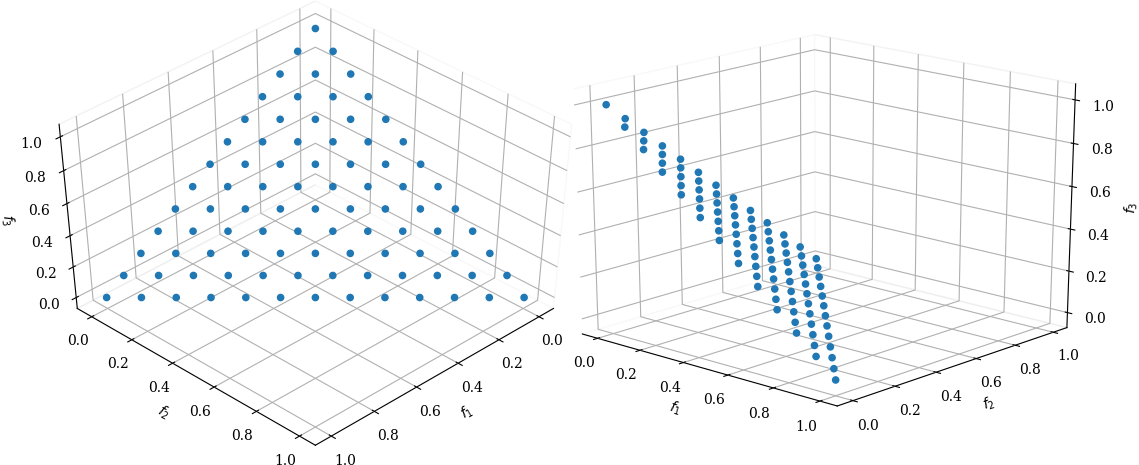
\includegraphics{refpoints.eps}}
\caption{Reference points in 3 dimensions, partition-size 12}
\label{fig:refpoints}
\end{figure}

The discovered pareto-front is
projected onto this hyperplane \cite{BDR19}. When specifying reference
directions, these are directly defined in the objective space (without
any projection).

To compute a set of points we use an algorithm
originally defined in a paper by I.~Das and J.~E.~Dennis \cite{DD98}
with the function \verb+LIN_dasdennis+. This function gets the dimension
(the number of objectives to optimize which is the number of auxiliary
evaluations +1 minus the number of constraints) and the number of
partitions. It returns the points in \verb+result+ and optionally takes
a scale factor in the range 0..1 and a direction to shift this scaled
set of points. The direction is only needed if the scale factor is less
than one. The first time the function is called, the result must
point at a NULL pointer. The function automatically allocates the
necessary memory. It can be called multiple times to extend the points
already allocated. The resulting points are then passed into the
function \verb+PGASetReferencePoints+:

\begin{verbatim}
int npoints = 0;
void *result = NULL;
double point [3] = {1, 1, 1};

PGASetNumAuxEval (ctx, 2);
PGASetNumConstraint (ctx, 0);
npoints = LIN_dasdennis (3, 2, &result, 0, 1, NULL);
npoints = LIN_dasdennis (3, 1, &result, npoints, 0.5, point);
PGASetReferencePoints (ctx, npoints, result);
\end{verbatim}

For defining reference directions, the function
\verb+PGASetReferenceDirections+ is used. It gets the number of
directions and the vector of directions (each direction is a vector of
the dimensionality of the number of objectives) and the number of
partitions (for Das/Dennis points) and the scale factor of the generated
points:

\begin{verbatim}
    double directions [][3] = {{1, 1, 1}, {1, 2, 3}};
    PGASetReferenceDirections (ctx, 2, directions, 12, 0.05);
\end{verbatim}

The difference to the reference points above is that the
reference directions are in the objective space and the Das/Dennis
points are generated dynamically in each generation.

Note that by default when no population size if specified, NSGA-III uses
the number of points defined by the reference points and reference
directions for the population size.

The NSGA-III replacement optimizes the solutions to be near the
reference points and/or reference directions. With a high number
of objective functions, the N-dimensional space forming the solution
space increases exponentially with the number of objective functions.
This is known as the ``curse of dimensionality''. With NSGA-II it is
increasingly hard to find a well distributed set of solutions with more
than two or three objectives.  With the NSGA-III
replacement it is possible to concentrate the search to a predefined
number of reference points or reference directions.

\pga\ supports both GRGA and SSGA and variants in between via {\em
parameterized} population replacement.  For example, the {\tt PGASet} calls
\begin{verbatim}
PGASetPopSize         (ctx,200);
PGASetNumReplaceValue (ctx,10);
PGASetPopReplaceType  (ctx, PGA_POPREPL_BEST);
\end{verbatim}
specify that each generation a new population is created consisting of ten
strings created via recombination, and the 190 most fit strings from the old
population.  The 190 strings can also be selected
randomly, with or without replacement, by setting the second argument of {\tt
PGASetPopReplaceType} to \verb+PGA_POPREPL_RANDOM_REP+ or
\verb+PGA_POPREPL_RANDOM_NOREP+, respectively.

For selecting restricted
tournament replacement \verb+PGA_POPREPL_RTR+ is used. The default for
the window size (number of members of the old population that are chosen
for comparison with a new candidate) is \hbox{min $(n, N/20)$} where $n$
is the string length and $N$ is the population size \cite{Pel05}.
The window size can be set or queried
with \verb+PGASetRTRWindowSize+ and \verb+PGAGetRTRWindowSize+,
respectively. Note that when restricted tournament replacement is in
use, the maximum number of new candidates is limited with the number set
with \verb+PGASetNumReplaceValue+ but fewer---depending on fitness--may
be replaced into the new population. Note that it depends on the
selection which individuals in the old population are replaced. Since
restricted tournament replacement is an elitist strategy the overall
fitness never dimishes with this replacement strategy.

For pairwise best replacement \verb+PGA_POPREPL_PAIRWISE_BEST+ is used
as the replacement type. Like restricted tournament replacement it is an
elitist strategy.

For NSGA-II replacement \verb+PGA_POPREPL_NSGA_II+ is used. For NSGA-II
replacement \verb+PGA_POPREPL_NSGA_III+ is used.  The number
of auxiliary evaluation function can be set with \verb+PGASetNumAuxEval+
and the number of constraints can be set with \verb+PGASetNumConstraint+.
If the difference between the two is $>0$ (i.e. the number of objectives
is $>1$), these auxiliary evaluations are used for multi-objective
optimization. Only the NSGA-II and NSGA-III replacement are possible
with these settings (i.e. when the number of objectives is $>1$).

The replacement types \textit{pairwise best}, \textit{restricted tournament
replacement}, NSGA-II, and NSGA-III replacement have selection pressure
in addition to providing
a population replacement strategy. So these can be used if a selection
scheme without selection pressure (a tournament strategy with only one
participant in the tournament or linear selection) is used.

By default, the number of new strings created each generation is 10 percent
of the population size (an SSGA population replacement strategy).  A GRGA can
be implemented by setting {\tt PGASetNumReplaceValue} to the population size
(the default population size is 100).  Setting {\tt PGASetNumReplaceValue} to
one less than the population size will result in an elitist GRGA, where the
most fit string is always copied to the new population (since {\tt
PGA\_POPREPL\_BEST} is the default population replacement strategy).

Traditionally, strings created through recombination first undergo crossover
and then mutation.  Some practitioners \cite{Da91} have argued that these two
operators should be separate.  By default, \pga\ applies mutation only to
strings that did {\em not} undergo crossover.

\begin{sloppypar}
This is equivalent to setting \verb+PGASetMixingType+ to
\verb+PGA_MIX_MUTATE_OR_CROSS+ which is also the default.
To have strings undergo {\em both} crossover and mutation, one should
set \verb+PGASetMixingType+ to \verb+PGA_MIX_TRADITIONAL+. Note that
there is also a mode that will not mutate strings that are not also
crossed over. This can be enabled by setting \verb+PGASetMixingType+ to
\verb+PGA_MIX_MUTATE_AND_CROSS+.
\end{sloppypar}

If an evolutionary algorithm variant without crossover is used or if
special crossover techniques with more that two parents should be
applied, all the logic can be implemented in a custom crossover operator
and the \verb+PGASetMixingType+ can be set to \verb+PGA_MIX_MUTATE_ONLY+.
In this mode no crossover is performed at all.

There is also a legacy interface which should \textit{not} be used for
new code. Functions used in that interface are:
\verb+PGASetMutationOrCrossoverFlag+,
\verb+PGASetMutationAndCrossoverFlag+, and
\verb+PGASetMutationOnlyFlag+.

By default, \pga\ allows duplicate strings in the population.  Some
practitioners advocate not allowing duplicate strings in the population in
order to maintain diversity.  The function call {\tt PGASetNoDuplicatesFlag}
{\tt (ctx,PGA\_TRUE)} will not allow duplicate strings in the population: It
repeatedly applies the mutation operator (with an increasing mutation rate) to
a duplicate string until it no longer matches any string in the new
population.  If the mutation rate exceeds 1.0, however, the duplicate string
{\em will} be allowed in the population, and a warning message will be issued.

Figure~\ref{fig:popreplace} shows the generic population replacement scheme in
\pga.  Both populations $k$ and $k+1$  are of fixed size (the value returned by
{\tt PGAGetPopSize}).  First, {\tt PGAGetPopSize} - {\tt
PGAGetNumReplaceValue} strings are copied over directly from generation $k$.
The way the strings are chosen, the most fit, or randomly with or without
replacement, depends on the value set by {\tt PGASetPopReplaceType}.  The
remaining {\tt PGAGetNumReplaceValue} strings are created by crossover and
mutation.

\begin{figure}
\centerline{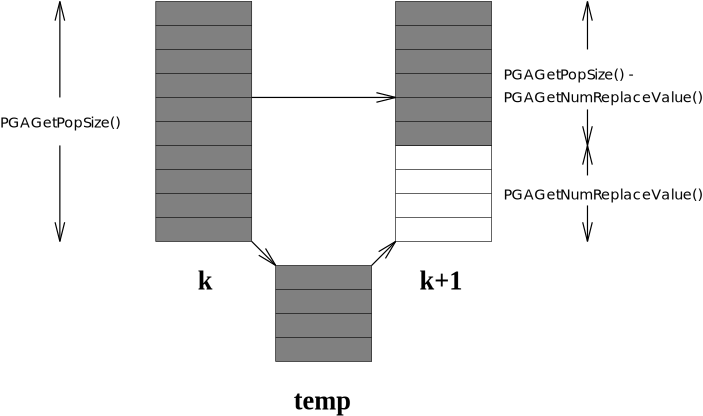
\includegraphics{generation.eps}}
\caption{Population Replacement}\label{fig:popreplace}
\end{figure}


%*****************************************************************************
\section{Stopping Criteria}\label{sec:stopping-criteria}
%*****************************************************************************

\pga\  terminates when at least one of the stopping
rule(s) specified has been met.  The three stopping rules are (1) iteration
limit exceeded, (2) population too similar, and (3) no change in the best
solution found in a given number of iterations.  The default is to stop when
the iteration limit (by default, 1000 iterations) is reached. Note that
when $\epsilon$-constraint optimization is in use, stopping is not
triggered as long as $\epsilon>0$, see section~\ref{sec:evaluation}.

\begin{sloppypar}
The choice of stopping rule is set by {\tt PGASetStoppingRuleType}.  For
example, {\tt PGASetStoppingRuleType} {\tt (ctx,PGA\_STOP\_MAXITER)} is the
default.  Other choices are {\tt PGA\_STOP\_TOOSIMILAR} and {\tt
PGA\_STOP\_NOCHANGE} for population too similar and no change in the best
solution found, respectively.  {\tt PGASetStoppingRuleType} may be called more
than once. The different stopping rules specified are {\em or}ed together.
\end{sloppypar}

If {\tt PGA\_STOP\_MAXITER} is one of the stopping rules, {\tt
PGASetMaxGAIterValue(ctx,500)} will change the maximum iteration limit to 500.
If {\tt PGA\_STOP\_NOCHANGE} is one of the stopping rules, {\tt
PGASetMaxNoChangeValue (ctx,50)} will change from 100 (the default) to 50 the
maximum number of iterations in which no change in the best evaluation is
allowed before the GA stops.  If {\tt PGA\_STOP\_TOOSIMILAR} is one of the
stopping rules, {\tt PGASetMaxSimilarityValue(ctx,99)} will change from 95 to
99 the percentage of the population allowed to have the same evaluation
function value before the GA stops.


%*****************************************************************************
\section{Initialization}\label{sec:initialization}
%*****************************************************************************

Strings are either initialized randomly (the default),
or set to zero.  The choice is specified by setting the second argument of
{\tt PGASetRandomInitFlag} to either {\tt PGA\_TRUE} or {\tt PGA\_FALSE},
respectively.  Random initialization depends on the datatype.

If binary-valued strings are used, each gene is set to {\tt 1} or {\tt 0} with
an equal probability.  To set the probability of randomly setting a bit to
{\tt 1} to 0.3, use {\tt PGASetBinaryInitProb(ctx,0.3)}.

For integer-valued strings, the default is to set the strings to a permutation
on a range of integers.  The default range is $[0,L-1]$, where $L$ is the
string length.  {\tt PGASetIntegerInitPermute(ctx, 500, 599)} will set the
permutation range to $[500,599]$.  The length of the range {\em must} be the
same as the string length.

Alternatively, {\tt PGASetIntegerInitRange} will set each gene to a random value
selected uniformly from a specified range.  For example, the code
\begin{verbatim}
stringlen = PGAGetStringLength(ctx);
for(i=0;i<stringlen;i++) {
    low[i]  = 0;
    high[i] = i;
}
PGASetIntegerInitRange(ctx, low, high);
\end{verbatim}
will select a value for gene {\tt i} uniformly randomly from the interval
{\tt [0,i]}.

If real-valued strings are used, the alleles are set to a value selected
uniformly randomly from a specified interval.  The interval may be specified
with either the {\tt PGASetRealInitRange} or {\tt PGASetRealInitPercent}
functions.
For example, the code
\begin{verbatim}
stringlen = PGAGetStringLength(ctx);
for(i=0; i<stringlen; i++) {
    low[i]  = -10.0;
    high[i] = (double) i;
}
PGASetRealInitRange(ctx, low, high);
\end{verbatim}
will select a value for allele {\tt i} uniformly randomly from the interval
$[-10.0,{\tt i}]$.  This is the default strategy for initializing real-valued
strings.  The default interval is $[0,1.0]$.

{\tt PGASetRealInitPercent} specifies the interval with a median value and
percent offset.  For example,
\begin{verbatim}
stringlen = PGAGetStringLength(ctx);
for(i=1; i<=stringlen; i++) {
    median  [i-1] = (double)  i;
    percent [i-1] =          .5;
}
PGASetRealInitPercent(ctx, median, percent);
\end{verbatim}
will select a value for allele {\tt i} uniformly randomly from the increasing
intervals $[\frac{1}{2}i,\frac{3}{2}i]$.  Note that if
the median value is zero for some $i$, then an
interval of $[0,0]$ will be defined.

If character-valued strings are used,
{\tt PGASetCharacterInitType(ctx,PGA\_CINIT\_UPPER)} will set the  allele values
to uppercase alphabetic characters chosen uniformly randomly.
Other options are
{\tt PGA\_CINIT\_LOWER} for lower case letters only (the default) and 
{\tt PGA\_CINIT\_MIXED} for mixed case letters, respectively.

%*****************************************************************************
\section{Selection}\label{sec:selection}
%*****************************************************************************

The selection phase allocates reproductive trials to strings on the basis of
their fitness.  \pga\ supports five selection schemes: proportional selection,
stochastic universal selection, truncation selection, tournament
selection (default is binary tournament selection), and probabilistic
binary tournament selection. A sixth scheme which is called
\textit{linear selection} that is not a selection scheme in
the genetic sense (it has no selection pressure) is used for
evolutionary algorithms that rely on modification of individuals that
later replace their parent if the offspring has higher fitness, so the
selection pressure is applied in the replacement strategy. The linear
scheme is guaranteed to return individuals in population order.

\begin{sloppypar}
The choice may be specified by setting the
second argument of {\tt PGASetSelectType} to one of
\verb+PGA_SELECT_PROPORTIONAL+, \verb+PGA_SELECT_SUS+,
\verb+PGA_SELECT_TRUNCATION+, \verb+PGA_SELECT_TOURNAMENT+,
\verb+PGA_SELECT_PTOURNAMENT+, and \verb+PGA_SELECT_LINEAR+
for proportional, stochastic universal, truncation, tournament,
probabilistic tournament selection, and linear selection, respectively.
The default is tournament selection. For tournament
selection, the size of the tournament (number of participants) can be
set e.g., with \verb+PGASetTournamentSize(ctx, 3)+. The default is binary
tournament (size = 2). To allow a more fine-grained selection pressure,
the tournament size is a floating-point value. The integer part of
that value specifies the minimum tournament size. For each tournament
for the fractional part, a biased coin is flipped (using \verb+PGARandomFlip+)
and the tournament size is increased by one if the outcome is positive.
This mechanism for fine-grained tournaments was first proposed by Harik
and Goldberg \cite{HG96} and later rediscovered by Filipovi\'{c}
et.~al.\ \cite{FKTL00}.

Note that with a tournament size of 1 (or with
the linear selection scheme) there is no
selection pressure. Having no selection pressure in this step can be
compensated by using a replacement scheme with selection pressure, i.e.,
one of restricted tournament replacement or pairwise best replacement,
see section~\ref{sec:population-replacement} for details on population
replacement. If no selection pressure is used in the selection scheme
\textit{and} in the population replacement strategy, the genetic search
degenerates to a random walk.
\end{sloppypar}

In addition, for tournament selection it can be
specified if the selection is \textit{with} or \textit{without}
replacement using the function \verb+PGASetTournamentWithReplacement+ with
a parameter of \verb+PGA_FALSE+ or \verb+PGA_TRUE+. Sampling without
replacement guarantees that for $n$ tournaments, each individual
participates in the same number of tournaments (as long as $n$
multiplied by the tournament size is a multiple of the population size)
\cite{GKD89}. The was later re-invented by Sokolov and Whitley under
the name \textit{Unbiased Tournament Selection} \cite{SW05}.

The default sampling is
\texttt{with} replacement as if \verb+PGASetTournamentWithReplacement+
had been called with the parameter \verb+PGA_TRUE+.  The probabilistic
tournament selection is always binary (two participants in the
tournament), the default probability that the string that wins the
tournament is selected is 0.6.  It may be set to 0.8, for example, with {\tt
PGASetPTournamentProb(ctx, 0.8)}. The tournament for probabilistic
tournament selection is always with replacement. The truncation selection
by default selects half of the population. This proportion of selected
individuals can be set with \verb+PGASetTruncationProportion+ for which
the default value is 0.5.

When using multi-objective optimization with, e.g., the NSGA-II \cite{DPAM02}
population replacement (see section~\ref{sec:population-replacement}),
it is possible to either use a selection scheme with or without
selection pressure. However, selection schemes that rely on direct
comparison of individuals (e.g. tournament selection) will sort by the
domination rank of the individuals established by the NSGA-II algorithm.
This is because for multi-objective optimization there is no full order
established by multiple objectives as would be the case for
single-objective optimization. This may result in less selection
pressure because multiple individuals will typically have the same rank.
This lower selection pressure is compensated by the selection pressure
introduced by the NSGA-II (or -III) population replacement algorithm.

Most selection schemes (except stochastic universal selection) already
return a randomized sequence. In previous implementations \textit{all}
sequences got an additional randomization step. By default this is no
longer the case (exect for \verb+PGA_SELECT_SUS+). You can enable the
previous behavior by setting it to \verb+PGA_TRUE+ with
\verb+PGASetRandomizeSelect+. Note that even with this flag set, the
sequence returned by the linear selection scheme is never randomized.
This has adverse effects on crossover with linear selection:
With this scheme the same two adjacent population members are always
crossed over which makes crossover almost ineffective.
Linear selection is typically only useful when using special
mutation operators most often with \verb+PGASetMixingType+ set to
\verb+PGA_MIX_MUTATE_ONLY+.
If you need a randomized sequence without selection pressure, use
tournament selection without replacement with a tournament size of one.


% Baker's stochastic universal selection (SUS) is an optimal sampling algorithm
% \cite{Ba87}.  SUS may be thought of as constructing a roulette wheel using
% fitness proportionate selection and then spinning the wheel once, where the
% number of equally spaced markers on the wheel is equal to the population size.
% This method guarantees that each string is allocated $\lfloor expected value
% \rfloor$ reproductive trials and no more than $\lceil expected value
% \rceil$.
% 
% In {\em binary} tournament selection \cite{Go89,GoDe91} two strings are chosen
% randomly from the population.  The more fit string is then allocated a
% reproductive trial.  In order to produce an offspring, two binary tournaments
% are held, each of which produces one parent string.  These two parent strings
% then recombine to produce an offspring.  A variation of binary tournament
% selection is {\em probabilistic} binary tournament selection where the more
% fit string is selected with a probability $p_b$, $.5
% \leq p_b < 1$.  Probabilistic binary tournament selection does
% allow for the possibility that the best string in the population may be lost.
% Its advantage is a reduction in the selective pressure.

%*****************************************************************************
\section{Crossover}\label{sec:crossover}
%*****************************************************************************

\begin{sloppypar}
The crossover operator takes bits from each parent string and
combines them to create child strings.  
%Figure~\ref{fig:one-point-crossover} illustrates one-point
%crossover operator. Starting with two parent strings of length $n=8$, a
%crossover site $c=3$ is chosen at random. Two new strings are then created;
%one uses bits 1--2 from the first parent string and bits
%3--8 from the second parent string; the other string uses the
%complementary bits from the two parent strings.
%
%\begin{figure}[tb]
%\begin{verbatim}
%        Parent Strings                    Child Strings
%        a a a a a a a a                   a a b b b b b b
%        b b b b b b b b                   b b a a a a a a
%\end{verbatim}
%\centering
%\caption
%{
%One-Point Crossover\label{fig:one-point-crossover}
%}
%\end{figure}
%
%Figure~\ref{fig:two-point-crossover} illustrates two-point crossover. Starting
%with two parent strings of length $n=8$, two crossover sites $c_1=3$ and
%$c_2=6$ are chosen at random. Two new strings are then created; one uses bits
%1--2 and 6--8 from the first parent string and bits 3--5 from the second parent
%string; the other string uses the complementary bits from each parent string.
%
%\begin{figure}
%\begin{verbatim}
%        Parent Strings                    Child Strings
%        a a a a a a a a                   a a b b b a a a
%        b b b b b b b b                   b b a a a b b b
%\end{verbatim}
%\centering
%\caption
%{
%Two-Point Crossover\label{fig:two-point-crossover}
%}
%\end{figure}
%
%Figure~\ref{fig:uniform-crossover} illustrates uniform crossover. Starting
%with two parent strings of length $n=8$, the bit-mask {\tt 01101001} is
%randomly generated.  This mask is applied to the parent strings such that a
%``{\tt 1}'' bit indicates that the next bit for the first child string should
%be taken from the first parent string, and a ``{\tt 0}'' bit indicates that
%the next bit for the first child string should be taken from the second parent
%string.  The bit-string is then complemented and the process repeated to
%create the second child string.
%
%\begin{figure}
%\begin{verbatim}
%        Parent Strings                    Child Strings
%        a a a a a a a a                   b a a b a b b a
%        b b b b b b b b                   a b b a b a a b
%\end{verbatim}
%\centering
%\caption
%{
%Uniform Crossover\label{fig:uniform-crossover}
%}
%\end{figure}
%
The type of crossover may be specified by setting \verb+PGASetCrossoverType+
to \verb+PGA_CROSSOVER_ONEPT+, \verb+PGA_CROSSOVER_TWOPT+,
\verb+PGA_CROSSOVER_UNIFORM+, or \verb+PGA_CROSSOVER_SBX+ for one-point,
two-point, uniform, or simulated binary (SBX) crossover,
respectively. For integer alleles there is \verb+PGA_CROSSOVER_EDGE+ for
Edge Recombination crossover \cite{WSS91}. If the integer gene is
initialized to be a permutation, this variant preserves this property.
In addition some edges can be defined to be fixed (unmutable). This is
done with the \verb+PGAIntegerSetFixedEdges+. An example is given in
\verb+examples/sequence+.

The default is two-point crossover.  By default the crossover
rate is 0.85.  It may be set to 0.6 by {\tt PGASetCrossoverProb(ctx, 0.6)},
for example. Simulated binary crossover is available only for integer
and real genes.
\end{sloppypar}

Uniform crossover and simulated binary crossover are parameterized by
$p_u$, the probability of swapping two parent bit values \cite{SpDe91}
in the case of uniform crossover and for mutating an allele for SBX.
By default, $p_u = 0.5$.  The function call {\tt
PGASetUniformCrossoverProb(ctx, 0.7)} will set $p_u = 0.7$.

SBX uses a polynomial distribution with a parameter $\eta_c$ that defines
how far the child may deviate from each parent. For high values of this
parameter, children stay nearer to the parents \cite{DA95}. Recommended
values of this parameter are typically in the range 2--5, the default is
2 and a different value can be set with \verb+PGASetCrossoverSBXEta+.

When crossing strings with SBX, typically for each allele a new random
number is computed for the polynomial distribution. With
\verb+PGASetCrossoverSBXOncePerString+ you can define that a random
number is only drawn once for each individual to be crossed over.
This ensures that the child is on the line in N-dimensional space
between the two parents \textit{if all alleles are crossed over}.
This may be beneficial when handling optimization problems that are not
decomposable \cite{Sal96} similar to the crossover rate in differential
evolution \cite[p.~98]{PSL05}.

Crossover types that may yield child individuals outside the range of
the parents (currently only SBX) may want to call
\verb+PGASetCrossoverBoundedFlag+ or \verb+PGASetCrossoverBounceBackFlag+
with the context variable and \verb+PGA_TRUE+ to select an algorithm
that keeps the child alleles within the bounds of the initialization
ranges of the gene for each allele. These parameters work analogous to
\verb+PGASetMutationBoundedFlag+ and \verb+PGASetMutationBounceBackFlag+
for mutation. For the bounce-back implementation the parent
\textit{nearer} to the initialisation boundary is used for each check.


%*****************************************************************************
\section{Mutation}\label{sec:mutation}
%*****************************************************************************

The mutation {\em rate} is the probability that a gene will undergo
mutation.  The mutation rate is independent of the datatype used. The default
mutation rate is the reciprocal of the string length.  The function call {\tt
PGASetMutationProb(ctx,.001)} will set the mutation rate to .001.

The {\em type} of mutation depends on the data type.  For binary-valued
strings, mutation is a bit complement operation. For
character-valued strings, mutation replaces one alphabetic character with
another chosen uniformly randomly.  The alphabetic characters will be lower,
upper, or mixed case depending on how the strings were initialized.

For integer-valued strings, if the strings were initialized to a permutation
and gene $i$ is to be mutated, the default mutation operator swaps gene $i$
with a randomly selected gene. If the strings were initialized to a random
value from a specified range and gene $i$ is to be mutated, by default gene
$i$ will be replaced by a value selected uniformly random from the
initialization range.

The mutation operator for integer-valued strings may be changed irrespective
of how the strings were initialized.  If {\tt PGASetMutationType} is set to
{\tt PGA\_MUTATION\_RANGE}, gene $i$ will be replaced with a value selected
uniformly randomly from the initialization range.  If the strings were
initialized to a permutation, the minimum and maximum values of the
permutation define the range.  If {\tt PGASetMutationType} is set to {\tt
PGA\_MUTATION\_PERMUTE}, gene $i$ will be swapped with a randomly selected
gene.  If {\tt PGASetMutationType} is set to {\tt PGA\_MUTATION\_CONSTANT}, a
constant integer value (by default one) will be added (subtracted) to (from)
the existing allele value.  The constant value may be set to 34, for example,
with {\tt PGASetMutationIntegerValue (ctx,34)}.

Three of the real-valued mutation operators are of the form $v \leftarrow
v \pm p \times v$, where $v$ is the existing allele value.  They vary by how
$p$ is selected.  First, if {\tt PGASetMutationType} is set to {\tt
PGA\_MUTATION\_CONSTANT}, $p$ is the constant value 0.01. It may be set to
.02, for example, with {\tt PGASetMutationRealValue(ctx,.02)}.  Second, if
{\tt PGASetMutationType} is set to {\tt PGA\_MUTATION\_UNIFORM}, $p$ is
selected uniformly from the interval $(0,.1)$. To select $p$ uniformly from
the interval $(0,1)$ set {\tt PGASetMutationRealValue(ctx,1)}.  Third, if {\tt
PGASetMutationType} is set to {\tt PGA\_MUTATION\_GAUSSIAN}, $p$ is selected
from a Gaussian distribution (this is the default real-valued mutation
operator) with mean 0 and standard deviation 0.1.  To select $p$ from a
Gaussian distribution with mean 0 and standard deviation 0.5 set {\tt
PGASetMutationRealValue(ctx,.5)}.  Finally, if {\tt PGASetMutationType} is set
to {\tt PGA\_MUTATION\_RANGE}, gene $i$ will be replaced with a value selected
uniformly random from the initialization range of that gene.

For integer and real genes there is a polynomial mutation operator
selected with the mutation type constant \verb+PGA_MUTATION_POLY+
\cite{DG96}. It works by drawing a random number from a polynomial
probabilty density
function for a fixed mutation interval. The mutation interval by default
is between the current allele value and the lower/upper initialisation
range of the gene. Unless you also call \verb+PGASetMutationBoundedFlag+
or \verb+PGASetMutationBounceBackFlag+ to keep mutation within the
bounds of the initialization range, the default value does not make much
sense (because the current value may already exceed the boundary). In
that case (and other cases where you want a fixed mutation range) you
can call \verb+PGASetMutationPolyValue+ to set the mutation range. The
polynomial mutation distribution has a parameter $\eta_m$ that specifies how
likely values far away from the current allele are selected, the higher
this value gets, the nearer the mutated values stays to the parent. You
can set this parameter with \verb+PGASetMutationPolyEta+, the default is
100 \cite{DD14}.

\def\DefaultDEScaleFactor{0.9}
\def\DefaultDECrossoverProb{0.9}
\def\DefaultDEJitter{0.0}
\def\DefaultDEDither{0.0}
\def\DefaultDEProbabilityEO{0.5}
\def\DefaultDENumDiffs{1}

For Differential Evolution (DE), the strategy is implemented as the
mutation type \verb+PGA_MUTATION_DE+\label{mutation-de}. Note that for
the full DE algorithm not just a special mutation type is needed, see
section~\ref{sec:differential-evolution} for an introduction. You
typically want to chose mutation only, linear selection, and
pairwise-best replacement.
For DE, real-valued genes are typically called \textit{vectors} (because
a gene is a vector of real-valued alleles), we use that term in the
following.

The default strategy of DE is to compute the distance of a pair of
random vectors in the population and add this difference to a
randomly-chosen third vector:

\begin{equation}\label{de/rand/1}
V_{i,g} = X_{r_0,g} + F \cdot (X_{r_1,g} - X_{r_2,g})
\end{equation}

Where $g$ denotes the generation, $i$ is the running population
index, and $r_0$, $r_1$, and $r_2$ are random population indeces
different from each other and the running index $i$. The factor $F$,
called the scale factor, is a parameter of the search and can be
specified with \verb+PGASetDEScaleFactor+, the default is
\DefaultDEScaleFactor. The range for this parameter is $[0,2]$ but
typical values are in the range $[0.3,1)$, the exact
value $1.0$ should not be chosen because it reduces the number of
mutants and thus potentially the genetic variance \cite[p.~75]{PSL05}.

The resulting
mutant vector $V_i$, also called the \textit{donor} vector, is then
combined via crossover with the $i^{\hbox{\footnotesize th}}$ member of
the population $X_i$. Note that the crossover in this implementation of DE is
\textit{not} the normal genetic algorithm crossover (from
section~\ref{sec:crossover}), in fact when using DE, crossover is
typically turned off by setting \verb+PGASetMixingType+ to
\verb+PGA_MIX_MUTATE_ONLY+. Instead DE uses its own crossover implementation
within the \verb+PGA_MUTATION_DE+ mutation implementation. For each
vector element (allele), a random variable with a crossover probability
specified by \verb+PGASetDECrossoverProb+ (default \DefaultDECrossoverProb)
is chosen. In the default binomial crossover variant of DE this variable
selects an element from either the donor vector $V_i$ or $X_i$. In the
DE literature this parameter is typically called \textit{Cr}. At least
one random element from $V_i$ is always selected, so with a crossover
probability of 0, exactly one element from the donor vector is selected.
With a crossover probability of 1, \textit{all} elements from the donor
vector are selected. Crossover plays a significat role in optimisation.
For decomposable problems (where each dimension of the problem can be
optimized separately \cite{Sal96}) a low crossover rate $0 \le Cr \le
0.2$ is a good choice. For non-decomposable problem a high crossover
rate should be chosen, i.e. $0.9 \le Cr \le 1$ \cite[p.~98]{PSL05}.

The resulting individual after crossover is placed in the
new population. If pairwise-best population replacement is selected (the
default in the DE literature, see section~\ref{sec:population-replacement})
it is later compared with the old individual $X_i$ in the old population
which it replaces if it has better fitness.

There are different variants of DE and a notation was
established to distinguish these variants. The notation uses a 4-tuple
where each element is delimited with a '/'. The first element in the
tuple is always the string \textit{DE} for Differential Evolution. The second
element describes the variant. The most common (often called the
\textit{classic} variant) selects a random element from the population
for modification and is therefore called \textit{rand}, see
equation~\ref{de/rand/1}. The third tuple-element is the number of
difference-pairs applied to the modified element, it is typically one or
two. If we use two differences, the formula in equation~\ref{de/rand/1}
would become:
\begin{equation}\label{de/rand/2}
V_{i,g} = X_{r_0,g} + F \cdot (X_{r_1,g} - X_{r_2,g})
    + F \cdot (X_{r_3,g} - X_{r_4,g})
\end{equation}
The number of differences can be specified with \verb+PGASetDENumDiffs+
and defaults to 1. Note that not all DE strategies use this parameter.

The fourth final element specifies the crossover strategy. For the
default DE-crossover strategy following a binomial distribution (in
standard GA terms this type of crossover is often called
\textit{uniform} crossover) this final element is termed \textit{bin}.
The crossover for DE can be set with \verb+PGASetDECrossoverProb+. The
default is binomial crossover \verb+PGA_DE_CROSSOVER_BIN+, exponential
crossover can be set with \verb+PGA_DE_CROSSOVER_EXP+.
So for the default DE strategy the name is \textit{DE/rand/1/bin} with
the exponential crossover selected, we would get \textit{DE/rand/1/exp}.
Binomial crossover tosses a biased coin with probability $Cr$ for each
allele. If the coin turns out '1', the allele is taken from the donor
vector, otherwise the allele from the current individual is retained.
For exponential crossover an index in the gene is randomly selected and
taken from the donor vector. For all subsequent alleles (starting at the
randomly selected index) a coin is tossed. As long as the coin is '1',
the allele is taken from the donor vector. The first time the coin-toss
doesn't yield a '1', all the remaining alleles are taken retained from
the original individual. This is a form of two-point crossover like in
other types of genetic algorithms but with a different distribution.
The binomial crossover is beneficial if the allele positions in the
problem are uncorrelated. If there is a corellation between allele
positions, exponential crossover may be beneficial \cite{TF14}.

The DE variant (the second tuple element) can be selected with
\verb+PGASetDEVariant+ and defaults to \verb+PGA_DE_VARIANT_RAND+.
Another variant is the \textit{best} variant which uses the current best
individual for modification according to equation~\ref{de/best/1}. This
variant is selected with the contant \verb+PGA_DE_VARIANT_BEST+.

\begin{equation}\label{de/best/1}
V_{i,g} = X_{\hbox{\footnotesize best},g} + F \cdot (X_{r_1,g} - X_{r_2,g})
\end{equation}

A third variant called \textit{either-or} \cite[p.~117]{PSL05} is
selected with the constant \verb+PGA_DE_VARIANT_EITHER_OR+. It randomly
selects among a mutation operator and a recombination operator according
to equation~\ref{de/either-or/1}.

\begin{equation}\label{de/either-or/1}
V_{i,g} = \left\{
    \begin{array}{ll}
    {X_{r_0,g} + F \cdot (X_{r_1,g} - X_{r_2,g})}
        & \mbox{if rand$_i$(0, 1) $< p_F$} \\
    {X_{r_0,g} + K \cdot (X_{r_1,g} + X_{r_2,g} - 1\cdot X_{r_0,g})}
        & \mbox{otherwise} \\
    \end{array} \right.
\end{equation}

The probability $p_F$ defaults to \DefaultDEProbabilityEO{} and can be
set with \verb+PGASetDEProbabilityEO+. The parameter $K$ defaults to
$0.5 \cdot (F + 1)$ \cite[p.~118]{PSL05} where F is the scale factor, it
can be set with \verb+PGASetDEAuxFactor+. Note that the either-or
variant ignores the parameter specifying the number of difference
vectors (specified with \verb+PGASetDENumDiffs+). The expression
rand$_i$(0,~1) denotes a random number in the range $[0, 1)$ which is
re-generated for each individual $i$.

When computing the donor vector $V_i$, the scale factor $F$ can be
perturbed. This can either be done anew for each individual or for each
\textit{allele} of each individual. The first variant is called
\textit{dither} while the
second variant is called \textit{jitter}.  Note that jitter not only
changes the length of the difference vector but also its orientation
\cite[p.~80]{PSL05}.  With uniform jitter we get a new factor $F_j$, the
index $j$ denoting the allele while $i$ is the index of the current
individual \cite[p.~80]{PSL05}:

\def\jit{K_{\mbox{\footnotesize jit}}}
\def\dit{K_{\mbox{\footnotesize dit}}}
\begin{equation}\label{jitter}
\begin{array}{ll}
F_j = (F + \jit\cdot (\mbox{rand}_j(0, 1) - 0.5), & \jit < 2 \cdot F \\
\end{array}
\end{equation}

The same applies for dither, but in the case of dither the factor is
either applied anew for each individual (when setting
\verb+PGASetDEDitherPerIndividual+ to \verb+PGA_TRUE+) or only once per
generation (the default being once per generation), note that for the
case where the dither is applied once per generation the index $i$ of
$\jit{}$ in equation~\ref{dither} would refer the the generation:

\begin{equation}\label{dither}
\begin{array}{ll}
F_i = (F + \dit\cdot (\mbox{rand}_i(0, 1) - 0.5), & \dit < 2 \cdot F \\
\end{array}
\end{equation}

The new $F_j$ and/or $F_i$ replaces $F$ in
equations~\ref{de/rand/1}--\ref{de/either-or/1} and both, the default
$\jit$ and the default $\dit$ are zero by default.
If both are non-zero, both are applied. Defaults can
can be set with \verb+PGASetDEJitter+ and \verb+PGASetDEDither+,
respectively.
Very small amounts of uniformly distributed jitter (on the order of
0.001) have been recommended for some problems \cite[p.~90]{PSL05} like
digital filter design \cite[p.~440]{PSL05}. Likewise quite large amounts
of dither (on the order of 0.5) are recommended for these problems.

Some of the integer- and real-valued mutation operators may generate allele
values outside the initialization range of that gene.  By
default, the allele value will \textit{not} be reset to the lower
(upper) value of the
initialization range for that gene.  By setting
\verb+PGASetMutationBoundedFlag(ctx, PGA_TRUE)+ the allele values will
be set to the value of the bound if they fall outside of the
initialization range. It was argued that setting the value to the bound
would reduce the genetic variance and could lead to premature
convergence if several individuals get the same value \cite[p.~204]{PSL05}.
Therefore an alternative called ``Bounce-Back'' was proposed: If
\verb+PGASetMutationBounceBackFlag(ctx, PGA_TRUE)+ is set, the new value
is set to a random value between the old value and the bound.

A note on the use of the DE mutation type together with other selection
or replacements schemes: The DE mutation is very disruptive. It will not
work well or not work at all with a non-elitist replacement scheme. Due
to the high disruption, if not retaining at least one best individual
in each generation, it is very likely that the search will diverge. Good
choices for an elitist strategy are the two elitist replacement schemes
\verb+PGA_POPREPL_PAIRWISE_BEST+ (which is the standard replacement
scheme for Differential Evolution) and \verb+PGA_POPREPL_RTR+. The
latter may help if the algorithm stagnates due to premature convergence.
In that case RTR can help to retain more genetic diversity. For details
see section~\ref{sec:population-replacement}.


%*****************************************************************************
\section{Restart}\label{sec:restart}
%*****************************************************************************

The restart operator reseeds a population from the best string.  It does so by
seeding the new population with the best string and generating the remainder
of the population as mutated variants of the best string.

\begin{sloppypar}
By default the restart operator is not invoked.  Setting {\tt
PGASetRestartFlag(ctx,PGA\_TRUE)} will cause the restart operator to be
invoked.  By default \pga\ will restart every 50 iterations.  {\tt
PGASetRestartFrequencyValue} {\tt (ctx,100)} will restart every 100 iterations
instead.  When creating the new strings from the best string an individual
allele undergoes mutation with probability 0.5.  This can be changed to 0.9
with the function call {\tt PGASetRestartAlleleChangeProb(ctx,0.9)}.
\end{sloppypar}

For binary-valued strings the bits are complemented.  For integer- and
real-valued strings the amount to change is set with {\tt
PGASetMutationIntegerValue} and {\tt PGASetMutationRealValue}, respectively.
Character-valued strings are changed according to the rules in
Section~\ref{sec:mutation} for mutating character strings.

%*****************************************************************************
\section{String Evaluation and Fitness}\label{sec:evaluation}
%*****************************************************************************

In a genetic algorithm each string is assigned a nonnegative, real-valued {\em
fitness}.  This is a measure, relative to the rest of the population, of how
well that string satisfies a problem-specific metric.  In \pga\ calculating a
string's fitness is a two-step process.  First, the {\em user} supplies a
real-valued evaluation (sometimes called the raw fitness) of each string.
Second, this value is mapped to a fitness value.

It is the user's responsibility to supply a function to evaluate an individual
string.  As discussed in Section~\ref{sec:big-picture}, the name of this
function is specified as the second argument to {\tt PGARun}. The calling
sequence for this function (which we call {\tt evaluate} in the rest of this
section, but may have any name) {\em must} follow the format given here.  In C
the format is
\begin{verbatim}
double evaluate (PGAContext *ctx, int p, int pop, double *aux);
\end{verbatim}
and in Fortran
\begin{verbatim}
double precision function evaluate (ctx, p, pop, aux)
integer ctx, p, pop
double precision aux(*)
\end{verbatim}

The function {\tt evaluate} will be called by {\tt PGARun} whenever a string
evaluation is required.  {\tt p} is the index of the string in population {\tt
pop} that will be evaluated.  The correct values of {\tt p} and {\tt pop} will
be passed to the evaluation function by {\tt PGARun}.  (If {\tt PGARun} is not
used, {\tt PGAEvaluate} must be.  See Chapter~\ref{chp:explicit}.)
As shown below,  {\tt p}
and {\tt pop} are used for reading (and sometimes writing) allele values.
Sample evaluation functions
are shown in Figures~\ref{example:simple-main} and
\ref{example:maxbit-fortran}, and online in the {\tt ./examples} directory. 

In addition to returning just one evaluation, \pga\ supports
additional \textit{auxiliary} evaluations. The default use for this
mechanism is the specification of \textit{constraints} on the objective
function. If a problem does not allow all areas of the search space
because it may contain invalid solutions, additional restrictions on the
validity of points in the search space may be specified via constraints.

Another use-case for auxiliary evaluations is multiobjective
optimization: The algorithm is not just searching for \textit{one}
solution but for an array of objectives that can usually not all be
optimized to their optimum value. Instead a better value for one
objective may necessitate a worse value for another objective. A
multiobjective algorithm tries to find many \textit{non dominated}
solutions to a problem (a solution is said to dominate another solution
if it is better in at least one objective but not worse in any other
objective). These non-dominated solutions are said to lie on a
\textit{Pareto Front} after the mathematician Vilfredo Pareto who first
defined the concept today known as \textit{pareto optimality}.

\pga\ now implements multi-objective optimization with the Nondominated
Sorting Genetic Algorithm (Version~2) \cite{DPAM02} as a replacement
strategy. You can mix multi-objective optimization and constraints.
See below and section~\ref{sec:population-replacement} for details.

By default, auxiliary evaluations are used for constraints. All
auxiliary evaluation are summed if the value is positive. If it is zero
or negative, the constraint is not violated and not included in the sum.
So the algorithm is
minimizing constraint violations.  Individuals are sorted by the amount
of their constraint violations and the value of the objective function.
If an individual without constraint violations is compared to one with
constraint violations, the one without violations wins. For two
individuals with constraint violations the one with the lower sum of
violations wins. For two individuals without constraint violations the
normal comparison (depending on the direction of the search, i.e.
minimization or maximization) is used. This algorithm works better than
trying to code the constraint violations into a complicated evaluation
function. It was shown to work better than customized penalty functions
by Deb \cite{Deb00}.

With this algorithm for optimizing constraints, the constraints are
optimized first, only after solutions without constraint violations have
been found is the objective function considered. This has the drawback
that for certain problems the search will end up in a region of the
search space where the constraints are not violated but where no good
solutions exist. So with some problems the solutions found are very far
from the optimum. An idea by Takahama and Sakai \cite{TS10}, \cite{TS06}
introduces an $\epsilon$-constraint mechanism. An epsilon tolerance is
introduced and initialized with the constraint violation sum of the
$\theta$-best individual. The index of the individual $\theta$ can be
set with \verb+PGASetEpsilonTheta+, the default is $0.2$ the population
size.

The comparison of evaluations is modified to include an
$\epsilon$-tolerance: If both individuals have a constraint violation
below the tolerance, the evaluation is compared. If only one
individual exceeds the tolerance the other individual wins and if both
exceed the tolerance, the one with the lower constraint sum wins. The
$\epsilon$ is slowly decreased until it becomes zero at some generation
$T_c$. The slope of decrease can be specified with the
\verb+PGASetEpsilonExponent+ function, values between 2 (slow decrease)
and 10 (fast decrease) are possible. The default is an adaptive
algorithm for decrease of $\epsilon$ described in the 2010 paper \cite{TS06}
that works well in practise.

For using the $\epsilon$-constraint method, the generation $T_c$ until
which $\epsilon$ is decreased needs to be set using the
\verb+PGASetEpsilonGeneration+ function, the default is zero.
Note that \verb+PGASetEpsilonGeneration+ needs to be below the value set
with \verb+PGASetMaxGAIterValue+ even if the latter is not used as a
stopping criterion. Also note that the stopping criteria (see
section~\ref{sec:stopping-criteria}) are modified to not stop as long as
$\epsilon$ is not zero.

Auxiliary evaluations are returned in an array pointed to by the \verb+aux+
parameter of the users's evaluation function. To use auxiliary
evaluations, the number of auxiliary evaluations has to be specified
with the \verb+PGASetNumAuxEval+ function which gets the number of
auxiliary evaluations as the second parameter. The default is 0.
If you want to use multi-objective optimization, optionally with
constraints, you need to specify the number of constraints using the
\verb+PGASetNumConstraint+ function. By default the number of
constraints is equal to the number of auxiliary evaluations. So if you
want to use multi-objective evaluation you need to set the number of
constraints lower (optionally to zero if you have only multi-objective
optimization without constraints) than the number of auxiliary
evaluations.

Note that auxiliary evaluations can not be used together with selection
schemes that use mechanisms where individuals are not directly compared.
These currently are proportional selection and stochastic universal
selection, see section~\ref{sec:selection}.

Traditionally, genetic algorithms assume fitness values are nonnegative and
monotonically increasing the more fit a string is.  The user's evaluation of a
string, however, may reflect a minimization problem and/or be negative.
Most modern selection algorithms (e.g. the default tournament variants)
directly compare individuals and will directly use the users evaluation.
There are two selection mechanisms, \verb+PGA_SELECT_SUS+ and
\verb+PGA_SELECT_PROPORTIONAL+ which need a nonnegative and
monotonically increasing fitness. \textit{Only for these}
the user's {\em evaluation value} is mapped to a nonnegative and
monotonically increasing {\em fitness value}.

You may think of the algorithm used as follows (actually for the ranking
method the evaluation value is never translated):
First, all evaluations are
mapped to positive values (if any were negative).  Next, these values are
translated to a maximization problem (if the direction of optimization
specified was minimization).  Finally, these values are mapped to a fitness
value by using the identity (the default), linear ranking, or linear
normalization, The choice of fitness mapping may be set with the function
\verb+PGASetFitnessType+.  The second argument must be one of
\verb+PGA_FITNESS_RAW+, \verb+PGA_FITNESS_RANKING+, or
\verb+PGA_FITNESS_NORMAL+, for the identity, linear ranking, or linear
normalization, respectively.

Note that \verb+PGA_FITNESS_RAW+ and \verb+PGA_FITNESS_NORMAL+ are
subject to overflows if you have
very large (or very small negative) fitness values. If this occurs, an
error message is printed and the program terminates.
Letting the search continue with such an overflow would map many
\textit{different} evaluation values to the \textit{same} fitness.
For such ill-conditioned problems you should use the ranking
variant \verb+PGA_FITNESS_RANKING+.

A {\em linear rank} fitness function \cite{Ba87,Wh89} is given by
\begin{equation}
Min + (Max - Min)\cdot\frac{{\tt rank(p)}-1}{N-1},\label{eq:rank-select}
\end{equation}
where {\tt rank(p)} is the index of string {\tt p} in a list sorted in order
of decreasing evaluation function value, and $N$ is the population size.
Ranking requires that $1 \leq Max \leq 2$, and $Min + Max = 2$.  The default
value for $Max$ is 1.2.  It may be set to 1.1 with {\tt
PGASetMaxFitnessRank(ctx,1.1)}.

In {\em linear normalization} the fitness function is given by
\begin{equation}
K - ({\tt rank(p)} \cdot C),
\end{equation}
where $K$ and $C$ are the constants $\sigma \cdot N$ and $\sigma$,
where $\sigma$
is the standard deviation of the user's evaluation function values after they
have been transformed to positive values for a maximization problem.

If the direction of optimization is minimization, the values are remapped for
maximization.  The function call {\tt
PGASetFitnessMinType(ctx,PGA\_FITNESSMIN\_CMAX)} will remap by subtracting the
worst evaluation value from each evaluation value (this is the default).  The
worst evaluation value is multiplied by 1.01 before the subtraction so that
the worst string has a nonzero fitness.  The function call {\tt
PGASetFitnessCmaxValue (ctx, 1.2)} will change the multiplier to 1.2
Alternatively, if {\tt PGA\_FITNESSMIN\_RECIPROCAL} is specified the remapping
is done by using the reciprocal of the evaluation function.

Note that for algorithms that can directly compare individuals in the
selection method (any of the tournament selection methods, truncation
selection, and linear selection, see section~\ref{sec:selection}) or in
the replacement scheme (restricted tournament replacement or pairwise
best replacement, see section~\ref{sec:population-replacement}) do not
use the fitness but compare the evaluation value (and optionally the sum
of constraint violations) directly.

\section{Accessing Allele Values}\label{sec:allele-access}

For each of the native data types, \pga\ provides a matched pair of functions
that allow the user to read or write (change) any allele value.  If the data
type is {\tt PGA\_DATATYPE\_BINARY}
\begin{verbatim}
int bit;
bit = PGAGetBinaryAllele (ctx, p, pop, i);
\end{verbatim}
will assign to {\tt bit} the binary value of the {\tt i}th gene in string {\tt
p} in population {\tt pop}.  To set the {\tt i}th gene in string {\tt p} in
population {\tt pop} to {\tt 1}, use
\begin{verbatim}
PGASetBinaryAllele(ctx, p, pop, i, 1);
\end{verbatim}

If the data type is {\tt PGA\_DATATYPE\_INTEGER}
\begin{verbatim}
int k;
k = PGAGetIntegerAllele (ctx, p, pop, i);
\end{verbatim}
will assign to {\tt k} the integer value of the {\tt i}th gene in string
{\tt p} in population {\tt pop}.  
To set the {\tt i}th gene in string
{\tt p} in population {\tt pop} to 34, use
\begin{verbatim}
PGASetIntegerAllele(ctx, p, pop, i, 1, 34);
\end{verbatim}

If the data type is {\tt PGA\_DATATYPE\_REAL}
\begin{verbatim}
double x;
x = PGAGetRealAllele (ctx, p, pop, i);
\end{verbatim}
will assign to {\tt x} the real value of the {\tt i}th gene in string {\tt p}
in population {\tt pop}.
To set the {\tt i}th gene in string
{\tt p} in population {\tt pop} to 123.456, use
\begin{verbatim}
PGASetRealAllele(ctx, p, pop, i, 1, 123.456);
\end{verbatim}


If the data type is {\tt PGA\_DATATYPE\_CHARACTER}
\begin{verbatim}
char c;
c = PGAGetCharacterAllele (ctx, p, pop, i);
\end{verbatim}
will assign to {\tt c} the character value of the {\tt i}th gene in string
{\tt p} in population {\tt pop}.  To set the {\tt i}th gene in string {\tt p}
in population {\tt pop} to ``Z'', use
\begin{verbatim}
PGASetCharacterAllele(ctx, p, pop, i, 1, 'Z');
\end{verbatim}


\subsection{Representing an Integer with a Binary String}
\label{subsec:encode-integer}

A binary string may be used to represent an integer by {\em decoding} the
bits into an integer value.  In a binary coded decimal (BCD) representation, a
binary string is decoded into an integer $k
\in [0,2^{N}-1]$ according to
\begin{equation}
k = \sum_{i=1}^{N} b_{i} 2^{i-1},
\label{eq:bit}
\end{equation}
where $N$ is the string length, and $b_i$ the value of the $i$th bit.
For example, to decode the integer {\tt k} from the ten bits in bit positions
20--29, use
\begin{verbatim}
int k
k = PGAGetIntegerFromBinary(ctx,p,pop,20,29);
\end{verbatim}
The function {\tt PGAEncodeIntegerAsBinary} will encode an integer as a binary
string.  For example, to encode the integer 564 as a 12-bit binary
string\footnote{Even though only ten bits are necessary to encode 564, the
user may want to allow the GA any value between $[0,4095]$, hence the twelve
bits.}  in the substring defined by bits 12--23, use
\begin{verbatim}
PGAEncodeIntegerAsBinary(ctx,p,pop, 12, 23, 564);
\end{verbatim}

In a BCD representation, two numbers that are contiguous in their decimal
representations may be far from each other in their binary representations.
For example, 7 and 8 are consecutive integers, yet their 4-bit binary
representations, {\tt 0111} and {\tt 1000}, differ in the maximum number of
bit positions.\footnote{Technically, this is known as a Hamming cliff.}  {\em
Gray codes} define a different mapping of binary strings to integer values
from that given by Eq.~(\ref{eq:bit}) and may alternatively be used for
representing integer (or real, see below) values in a binary string.  The
second and third columns in Table~\ref{tab:gray-code} show how the integers
0--7 are mapped to Eq.~(\ref{eq:bit}) and to the {\em binary reflected} Gray
code (the most commonly used Gray code sequence), respectively.  In the binary
reflected Gray code sequence, the binary representations of consecutive
integers differ  by only one bit (a Hamming distance of one).

To decode the integer {\tt k} from a binary reflected Gray code
interpretation of the binary string, use
\begin{verbatim}
k = PGAGetIntegerFromGrayCode(ctx,p,pop,20,29);
\end{verbatim}
To encode 564 as a 12-bit binary string in the substring defined by bits 12--23 using a Gray code, use
\begin{verbatim}
PGAEncodeIntegerAsGaryCode(ctx,p,pop, 12, 23, 564);
\end{verbatim}



\begin{table}
\centering
\caption
{
Binary and Gray Codes\label{tab:gray-code}
}
\begin{tabular}{|r|r|r|} \hline\hline
    $k$ &      Eq.~(\ref{eq:bit}) &    Gray code \\  \hline
{\tt 0} &        {\tt 000} &         {\tt 000} \\
{\tt 1} &        {\tt 001} &         {\tt 001} \\
{\tt 2} &        {\tt 010} &         {\tt 011} \\
{\tt 3} &        {\tt 011} &         {\tt 010} \\
{\tt 4} &        {\tt 100} &         {\tt 110} \\
{\tt 5} &        {\tt 101} &         {\tt 111} \\
{\tt 6} &        {\tt 110} &         {\tt 101} \\
{\tt 7} &        {\tt 111} &         {\tt 100} \\ \hline
\end{tabular}
\end{table}

\subsection{Representing a Real Value with a Binary String}
\label{subsec:encode-real}

A binary string may also be used to represent a real value.  The decoding of a
binary string to a real-value is a two-step process.  First, the binary string
is decoded into an integer as described in
Section~\ref{subsec:encode-integer}.  Next, the integer is mapped from the
discrete interval $[0,2^{N}-1]$ to the real interval $[L,U]$ by using the
formula
\begin{displaymath}
x = (k-a) \times (U-L)/(b-a) + L
\end{displaymath}
(and generalizing $[0,2^{N}-1]$ to $[a,b]$).  For example, to decode the {\tt
double} {\tt x} from the 20 bits given by the binary string stored in bit
positions 10--29 onto the interval $[-10.0,20.0]$, use
\begin{verbatim}
x = PGAGetRealFromBinary(ctx,p,pop,10,29,-10.0,20.0);
\end{verbatim}
To encode -18.3 on the interval $[-50.0,50.0]$
using a 20-bit BCD binary string, use
\begin{verbatim}
PGAEncodeRealAsBinary(ctx,p,pop,0,19,-50.0,50.0,-18.3);
\end{verbatim}
The functions {\tt PGAGetRealFromGrayCode} and 
{\tt PGAEncodeRealAsGrayCode} provide similar functionality for Gray-coded
strings.

\subsection{Example}
\label{subsec:example}

As an example, suppose the user has a real-valued function $f$ of three real
variables $x_1$, $x_2$, and $x_3$.  Further, the variables are constrained as
follows.
\begin{displaymath}
-10 \leq x_1 \leq 0 
\end{displaymath}
\begin{displaymath}
0   \leq x_2 \leq 10
\end{displaymath}
\begin{displaymath}
-10 \leq x_3 \leq 10
\end{displaymath}
The user wishes to use 10 bits for the binary representation of $x_1$ and
$x_2$, and 20 bits for the binary representation of $x_3$ (perhaps for higher
accuracy), and a Gray code encoding.  This may be done as follows.
\begin{verbatim}
#include "pgapack.h"
double grayfunc (PGAContext *ctx, int p, int pop);
double f        (double x1, double x2, double x3);
int main(int argc, char **argv)
{
    PGAContext *ctx; 
    ctx = PGACreate (&argc, argv, PGA_DATATYPE_BINARY, 40, PGA_MINIMIZE);
    PGASetUp        (ctx                                               );
    PGARun          (ctx, grayfunc                                     );
    PGADestroy      (ctx                                               );
    return;
}

double grayfunc (PGAContext *ctx, int p, int pop)
{
    double x1, x2, x3, v;
    x1 =  PGAGetRealFromGrayCode (ctx, p, pop,  0,  9, -10.,  0.);
    x2 =  PGAGetRealFromGrayCode (ctx, p, pop, 10, 19,   0., 10.);
    x3 =  PGAGetRealFromGrayCode (ctx, p, pop, 20, 39, -10., 10.);
    v  =  f(x1,x2,x3);
    return(v);
}
\end{verbatim}
In Fortran, the bit indices would be 1--10, 11--20, and 21--40, respectively.
The number of bits allocated for the binary representation determines the
accuracy with which the real value can be calculated.  Note in this
example  the function {\tt f} {\em need not be modified}; the function
{\tt grayfunc} is used as a ``wrapper'' to get variable values out of the GA
and return the value calculated by {\tt f}.

%*****************************************************************************
\section{Report Options}\label{sec:report}
%*****************************************************************************

\begin{sloppypar}
{\tt PGASetPrintFrequencyValue(ctx,40)} will print population statistics every
40 iterations.  The default is every ten iterations.  The best evaluation is
{\em always} printed.  To print additional statistics, set the second argument
of the function {\tt PGASetPrintOptions} to {\tt PGA\_REPORT\_ONLINE}, {\tt
PGA\_REPORT\_OFFLINE}, {\tt PGA\_REPORT\_WORST}, {\tt PGA\_REPORT\_AVERAGE},
{\tt PGA\_REPORT\_HAMMING}, or {\tt PGA\_REPORT\_STRING} to print the online
analysis, offline analysis, worst evaluation, average evaluation, Hamming
distance, or string itself, respectively.  {\tt PGASetPrintOptions} may be
called multiple times to specify multiple print options.
\end{sloppypar}


%*****************************************************************************
\section{Utility Functions}\label{sec:utility}
%*****************************************************************************

\subsection{Random Numbers}\label{subsec:random}

By default, \pga\ will seed its random number generator by using a value from the
system clock.  Therefore, each time \pga\ is run, a unique sequence of random
numbers will be used.  For debugging or reproducibility purposes, however, the
user may wish to use the same sequence of random numbers each time.  This may
be done using the function {\tt PGASetRandomSeed} to initialize the random
number generator with the same seed each time, for example, {\tt
PGASetRandomSeed(ctx,1)}.

\begin{sloppypar}
{\tt PGARandom01(ctx,0)} will return a random number generated uniformly on
$[0,1]$.  If the second argument is not {\tt 0}, it will be used to reseed the
random number sequence. {\tt PGARandomFlip} flips a biased coin.  For example,
{\tt PGARandomFlip(ctx,.7)} will return {\tt PGA\_TRUE} approximately 70\% of
the time.  {\tt PGARandomInterval(-10,30)} will return an integer value
generated uniformly on $[-10,30]$.  {\tt PGARandomUniform} {\tt
(ctx,-50.,50.)} will return a real value generated uniformly randomly on the
interval [-50,50].  {\tt PGARandomGaussian} {\tt (ctx,0.,1.)} will return a
real value generated from a Gaussian distribution with mean zero and standard
deviation one.
\end{sloppypar}


\subsection{Print Functions}\label{subsec:print-functions}

{\tt PGAPrintPopulation(ctx,stdout,pop)} will print the evaluation function
value, fitness value, and string for each member of population {\tt pop} to
{\tt stdout}. This function may not be called until {\em after} {\tt PGASetUp}
has been called. {\tt PGAPrintContextVariable(ctx,stdout)} will print the
value of all fields in the context variable to {\tt stdout}.  {\tt
PGAPrintIndividual(ctx,stdout,p,pop)} will print the evaluation function
value, fitness value, and string of individual {\tt p} in population {\tt pop}
to {\tt stdout}.  {\tt PGAPrintString(ctx,stdout,p,pop)} will print the string
of individual {\tt p} in population {\tt pop} to {\tt stdout}.  {\tt
PGAPrintVersionNumber(ctx)} will print the \pga\ version number.


\subsection{Miscellaneous}\label{subsec:other}

\begin{sloppypar}
{\tt PGAGetGAIterValue(ctx)} will return the current iteration of the
GA.  {\tt PGAGetBestIndex(ctx,pop)} ({\tt PGAGetWorstIndex}) will return
the index of the most (least) fit member of population {\tt pop}.
\end{sloppypar}

{\tt PGAUpdateOffline(ctx,pop)} ({\tt PGAUpdateOnline}) will update the offline
(online) analysis based on the new generation's results.  {\tt
PGAHammingDistance(ctx,pop)} returns a {\tt double}, which is the average
Hamming distance between the {\em binary} strings in population {\tt pop}.
The function call
\begin{verbatim}
PGAError(ctx, "popindex=", PGA_FATAL, PGA_INT, (void *)&popindex)
\end{verbatim}
will print the message ``popindex=-1'' (assuming the value of {\tt popindex}
is -1) and then exit \pga.  If the third argument had been {\tt PGA\_WARNING}
instead, execution would have continued.  In addition to {\tt PGA\_INT}, valid data
types are {\tt PGA\_DOUBLE}, {\tt PGA\_CHAR}, and {\tt PGA\_VOID}.


%*****************************************************************************
\section{Command-Line Arguments}\label{sec:cla}
%*****************************************************************************

\pga\ provides several  command-line arguments.
These are only available to C programs, although in some cases both C and
Fortran programs can achieve the equivalent functionality with function calls.
For example, {\tt PGAUsage(ctx)} provides the same functionality as the {\tt
-pgahelp} command line option.  See Chapter~\ref{chp:debug} for the function
call equivalents.

\begin{verbatim}
  -pgahelp            get this message
  -pgahelp   debug    list of debug options
  -pgadbg   <level>   set debug option
  -pgadebug <level>   set debug option
  -pgaversion         Print current PGAPack version number, parallel or
                      sequential, and debug or optimized
\end{verbatim}

%*****************************************************************************
\chapter{Explicit Usage}\label{chp:explicit}
%*****************************************************************************

This chapter discusses how the user may obtain greater control over the steps
of the GA by {\em not} using the {\tt PGARun} command, but instead calling the
data-structure-neutral functions directly.  One ramification of this is that
the {\tt PGARun} interface no longer masks some of the differences between
parallel and sequential execution.  The examples in this chapter are written
for sequential execution {\em only}.  Chapter~\ref{chp:parallel} shows how
they may be executed in parallel.


%*****************************************************************************
\section{Notation}
%*****************************************************************************

To understand the calling sequences of the functions discussed in
this chapter, one must know of the {\em existence} of certain data
structures and the user interface for accessing them.  It is {\em not}
necessary to know how these data structures are implemented, since that is
hidden by the user interface to \pga.

\pga\ maintains two populations: an {\em old} one and a {\em new} one.  The
size of each population is the value returned by {\tt PGAGetPopSize}.  In
addition, each population contains two temporary working locations.  The
string length is the value specified to {\tt PGACreate} and returned by {\tt
PGAGetStringLength}.

Formally, string $p$ in population $pop$ is referred to by the 2-tuple {\tt
(p,pop)} and the value of gene $i$ in that string by the 3-tuple {\tt
(i,p,pop)}.  In \pga, {\tt pop} {\em must} be one of the two symbolic
constants {\tt PGA\_OLDPOP} or {\tt PGA\_NEWPOP} to refer to the old or new
population, respectively.  At the end of each GA iteration, the function {\tt
PGAUpdateGeneration} makes sure these symbolic constants are remapped to the
correct population.  The string index {\tt p} must be either an integer
between 0 and $P-1$ (or 1 and $P$ in Fortran) or one of the symbolic constants
{\tt PGA\_TEMP1} or {\tt PGA\_TEMP2}, to reference one of the two temporary
locations, respectively.

%*****************************************************************************
\section{Simple Sequential Example}
%*****************************************************************************

The example in Figure~\ref{simple-example} is a complete \pga\ program that
does {\em not} use {\tt PGARun}.  It is an alternative way to write the main
program for the Maxbit example of Section~\ref{sec:simple-example}.  We refer
to it as a simple example because it uses {\tt PGARunMutationAndCrossover} to
encapsulate the recombination step.  The {\tt PGACreate} and {\tt PGASetUp}
functions were discussed in the last chapter.  {\tt PGASetUp} creates and
randomly initializes the initial population.  This population, referred to
initially by the symbolic constant {\tt PGA\_OLDPOP}, is evaluated by the {\tt
PGAEvaluate} function.  The third argument to {\tt PGAEvaluate} is the name of
the user's evaluation function.  The function prototype for {\tt evaluate}
must be as shown in Figure~\ref{simple-example} and discussed earlier in
Sections~\ref{sec:big-picture} and~ \ref{sec:evaluation}.  The {\tt
PGAFitness} function maps the user's evaluation function values into
fitness values.

The {\tt while} loop runs the genetic algorithm.  {\tt PGADone} returns {\tt
PGA\_TRUE} if any of the specified stopping criteria have been met, otherwise
{\tt PGA\_FALSE}.  {\tt PGASelect} performs selection on population {\tt
PGA\_OLDPOP}.  {\tt PGARunMutationAndCrossover} uses the selected strings to
create the new population by applying the crossover and mutation operators.
{\tt PGAEvaluate} and {\tt PGAFitness} evaluate and map to fitness values the
newly created population. {\tt PGAUpdateGeneration} updates the GA iteration
count and resets several important internal arrays (don't forget to call it!).
{\tt PGAPrintReport} writes out genetic algorithm statistics according to the
report options specified.  Note that the argument to {\tt PGAPrintReport} is
the old population, since after {\tt PGAUpdateGeneration} is called, the newly
created population is in {\tt PGA\_OLDPOP}.  Finally, {\tt PGADestroy}
releases any memory allocated by \pga\ when execution is complete.

The functions {\tt PGADone}, {\tt PGAUpdateGeneration}, and {\tt PGAEvaluate}
take an MPI communicator (see Appendix~\ref{app:par-background} and
Chapter~\ref{chp:parallel}) as an argument.  For {\em sequential} execution
the value {\tt NULL} should be specified for this argument.
A parallel, or sequential {\em and} parallel, version of this example is given
in Section~\ref{sec:par-explicit-usage}.

\begin{figure}
\begin{verbatim}
#include "pgapack.h"
double evaluate (PGAContext *ctx, int p, int pop, double *aux);

int main(int argc, char **argv)
{
    PGAContext *ctx; 

    ctx = PGACreate(&argc, argv, PGA_DATATYPE_BINARY, 100, PGA_MAXIMIZE);
    PGASetUp   (ctx);
    PGAEvaluate(ctx, PGA_OLDPOP, evaluate, NULL);
    PGAFitness (ctx, PGA_OLDPOP);
    
    while(!PGADone(ctx, NULL)) {
        PGASelect                 (ctx, PGA_OLDPOP);
        PGARunMutationAndCrossover(ctx, PGA_OLDPOP, PGA_NEWPOP);
        PGAEvaluate               (ctx, PGA_NEWPOP, evaluate, NULL);
        PGAFitness                (ctx, PGA_NEWPOP);
        PGAUpdateGeneration       (ctx, NULL);
        PGAPrintReport            (ctx, stdout, PGA_OLDPOP);
    }
    PGADestroy(ctx);
    return(0);
}
\end{verbatim}
\caption{Simple Example of Explicit Usage}
\label{simple-example}
\end{figure}


%*****************************************************************************
\section{Complex Example}
%*****************************************************************************

\begin{figure}
\begin{verbatim}
#include "pgapack.h"
double evaluate(PGAContext *ctx, int p, int pop, double *aux);

int main(int argc, char **argv)
{
    PGAContext *ctx; 
    int i, j, n, m1, m2, popsize, numreplace;
    double probcross;

    ctx = PGACreate(&argc, argv, PGA_DATATYPE_BINARY, 100, PGA_MAXIMIZE);
    PGASetUp(ctx);
    probcross  = PGAGetCrossoverProb(ctx);
    popsize    = PGAGetPopSize(ctx);
    numreplace = PGAGetNumReplaceValue(ctx);
    PGAEvaluate(ctx, PGA_OLDPOP, evaluate, NULL);
    PGAFitness (ctx, PGA_OLDPOP          );
    
    while(!PGADone(ctx, NULL)) {
        PGASelect (ctx, PGA_OLDPOP);
        PGASortPop(ctx, PGA_OLDPOP);
        n = popsize - numreplace;
        for ( i=0; i < n; i++ ) {
            j = PGAGetSortedPopIndex(ctx, i);
            PGACopyIndividual(ctx, j, PGA_OLDPOP, i, PGA_NEWPOP);
        }
        while (n < popsize) { 
            m1 = PGASelectNextIndex(ctx, PGA_OLDPOP);
            m2 = PGASelectNextIndex(ctx, PGA_OLDPOP);        
            if(PGARandomFlip(ctx, probcross)) {
                PGACrossover(ctx, m1, m2, PGA_OLDPOP, PGA_TEMP1, PGA_TEMP2, PGA_NEWPOP);
                PGAMutate (ctx,PGA_TEMP1,PGA_NEWPOP);
                PGAMutate (ctx,PGA_TEMP2,PGA_NEWPOP);
                PGACopyIndividual (ctx,PGA_TEMP1,PGA_NEWPOP,n,  PGA_NEWPOP);
                PGACopyIndividual (ctx,PGA_TEMP2,PGA_NEWPOP,n+1,PGA_NEWPOP);
                n += 2;
            }
            else {
                PGACopyIndividual (ctx, m1, PGA_OLDPOP, n,   PGA_NEWPOP);
                PGACopyIndividual (ctx, m2, PGA_OLDPOP, n+1, PGA_NEWPOP);
                n += 2;
            }
        }
        PGAEvaluate(ctx, PGA_NEWPOP, evaluate, NULL);
        PGAFitness (ctx, PGA_NEWPOP);
        PGAPrintReport(ctx, stdout, PGA_NEWPOP);
        PGAUpdateGeneration(ctx, NULL);
    }
    PGADestroy(ctx);
    return 0;
}
\end{verbatim}
\caption{Example of Explicit Usage}
\label{complex-example}
\end{figure}

The primary difference between the ``complex'' example in
Figure~\ref{complex-example} and the ``simple'' example in
Figure~\ref{simple-example} is that the steps encapsulated by {\tt
PGARunMutationAndCrossover} have been written out explicitly.  The function
{\tt PGASortPop} sorts a population according to the criteria specified by
{\tt PGASetPopReplaceType} (Section~\ref{sec:population-replacement}).
The sorted indices are accessed via {\tt PGAGetSortedPopIndex}.  In the
example, the five lines that follow {\tt PGASortPop} copy the strings that are
not created by recombination from the old population to the new population.

The {\tt while} loop that follows creates the remainder of the new population.
{\tt PGASelectNextIndex} returns the indices of the strings selected by {\tt
PGASelect}.  {\tt PGARandomFlip} flips a coin biased by the crossover
probability to determine whether the selected strings should undergo crossover
and mutation or should be copied directly into the new population.  {\tt
PGACrossover} uses the parent strings {\tt m1} and {\tt m2} from population
{\tt PGA\_OLDPOP} to create two child strings in the temporary locations {\tt
PGA\_TEMP1} and {\tt PGA\_TEMP2} in {\tt PGA\_NEWPOP} population.

{\tt PGAMutate} mutates the child strings and {\tt PGACopyIndividual}, then
copies them into the new population.  If the strings do not undergo crossover
and mutation, they are copied into the new population unchanged.  The rest of
the steps are the same as those in Figure~\ref{simple-example}, {\em except}
that for illustrative purposes we call {\tt PGAPrintReport} {\em before} {\tt
PGAUpdateGeneration}.  In that case we use population {\tt PGA\_NEWPOP} as the
population pointer.

%*****************************************************************************
\section{Explicit \pga\ Functions}
%*****************************************************************************

This section briefly discusses other functions not shown in the previous
examples or discussed in Chapter~\ref{chp:functionality}.  Additional
information about these and other \pga\ functions is contained in
Appendix~\ref{chp:function-bindings} (function bindings) and the {\tt
./examples} directory.

\verb+PGARunMutationAndCrossover+ and \verb+PGARunMutationOrCrossover+ perform
the recombination step.  The former applies mutation to strings that undergo
crossover.  The latter applies only mutation to strings that did not undergo
crossover. Note that this means that when
\verb+PGARunMutationAndCrossover+ is selected, strings that are not crossed over
(because the random process did not select the individuals for crossover
with the given crossover probability) will also \textit{not} be mutated!
If no crossover is wanted, \verb+PGARunMutationOnly+ can be used for
mutation only without crossover.

The restart operator described earlier in Section~\ref{sec:restart} can be
invoked explicitly with {\tt PGARestart(ctx, oldpop, newpop)}, where the best
string from population {\tt oldpop} is used to initialize population {\tt
newpop}.

\verb+PGADuplicate(ctx,p,PGA_NEWPOP,PGA_NEWPOP)+ returns \verb+PGA_TRUE+
if string \verb+p+ in population \verb+PGA_NEWPOP+ is a duplicate of any
of the strings in population \verb+PGA_NEWPOP+ which were inserted into
the hash table using \verb+PGAHashIndividual+. Note that this function
is defined only for population \verb+PGA_NEWPOP+.

\verb+PGAHashIndividual(ctx,p,PGA_NEWPOP)+ hashes individual p in
population \verb+PGA_NEWPOP+ for duplicate checking.

\verb+PGAChange(ctx, p, PGA_OLDPOP)+ repeatedly applies the mutation
operator to string \verb+p+ in population \verb+PGA_OLDPOP+ until at
least one mutation has occurred.

All functions related to duplicate checking do nothing if duplicate
checking has not been enabled with \verb+PGASetNoDuplicatesFlag+, the
function \verb+PGAGetNoDuplicatesFlag+ can be used for checking if
duplicate checking is enabled.

In \pga\ three  values are associated with each string: (1) the user's
evaluation function value, (2) a Boolean flag to indicate whether the
evaluation function value is up to date with respect to the actual string, and
(3) the fitness value.  If {\tt PGARun} is not used, the user must manage
these values explicitly.

\begin{sloppypar}
{\tt PGAEvaluate(ctx, PGA\_NEWPOP, evaluate, comm)} will execute the user's
evaluation function, {\tt evaluate}, on each string in population {\tt
PGA\_NEWPOP} that has changed (for example, from crossover) since its last
evaluation.  {\tt PGAEvaluate} will set both the evaluation function value and
associated Boolean flag automatically.  The argument {\tt comm} is an MPI
communicator.  Valid values are {\tt NULL} for an explicitly sequential
example, or any valid MPI communicator.  Depending on the number of processes
specified when the program was invoked, and the value of the {\tt comm}
argument, {\tt PGAEvaluate} may be run with one or more processes.  See
Chapter~\ref{chp:parallel} for further discussion.
\end{sloppypar}

{\tt PGAFitness} will calculate the population fitness values from the
evaluation function values.  It is an error to call {\tt PGAFitness} if {\em
all} the evaluation function values are not up to date.

These same three values may be read also.  {\tt PGAGetEvaluation(ctx, p,
PGA\_OLDPOP)} returns the evaluation function value. {\tt
PGAGetEvaluationUpToDateFlag(ctx, p, PGA\_OLDPOP)} returns {\tt PGA\_TRUE} or
{\tt PGA\_FALSE} to indicate whether the evaluation is up to date with the
actual string or not, respectively.  If \pga\ was compiled for debugging,{\tt
PGAGetEvaluation} will print a warning message if the evaluation is not up to
date.  {\tt PGAGetFitness(ctx, p, PGA\_OLDPOP)} returns the fitness value.

\begin{sloppypar}
At times, (e.g., applying a hill-climbing function) the user may need to
explicitly set the evaluation function value and associated Boolean flag
(fitness values can be calculated {\em only} by calling {\tt PGAFitness}).
{\tt PGASetEvaluation(ctx, p, PGA\_OLDPOP, 123.4)} will set the evaluation
function value to 123.4 and the associated Boolean flag to {\tt PGA\_TRUE}.
The Boolean flag may be set independently with {\tt
PGASetEvaluationUpToDateFlag}.  For example, {\tt PGASetEvaluationUpToDateFlag
(ctx, p, PGA\_OLDPOP, PGA\_FALSE)} sets the status of the Boolean flag of
string {\tt p} in population {\tt PGA\_OLDPOP} to out of date.
\end{sloppypar}

{\tt PGAMean(ctx, a, n)} returns the mean of the {\tt n} values in array {\tt
a}. {\tt PGAStddev(ctx, a, n, mean)} returns the standard deviation of the
{\tt n} values in array {\tt a} whose mean is {\tt mean}.  {\tt PGARank(ctx,
p, order, n)} returns an index that is the rank of string p as given by the
sorted array {\tt order} of length {\tt n}.

\begin{sloppypar}
{\tt PGAGetPrintFrequency(ctx)} returns the frequency with which GA statistics
are reported. {\tt PGAGetWorstIndex} {\tt (ctx, PGA\_OLDPOP)} returns the
index of the string in population {\tt PGA\_OLDPOP} with the worst evaluation
function value.  {\tt PGAGetBestIndex(ctx, PGA\_OLDPOP)} returns the index of
the string in population {\tt PGA\_OLDPOP} with the best evaluation function
value.
\end{sloppypar}


%*****************************************************************************
\chapter{Custom Usage: Native Data Types}\label{chp:custom1}
%*****************************************************************************

This chapter discusses how \pga\ may be extended by replacing some of the
standard \pga\ functions with user-defined functions for use with one of
\pga's four {\em native}  data types.  This can be done from both C and
Fortran. 

\section{Basics}

\begin{table}
\centering
\caption
{Customizeable Functions: Native Data Types\label{tab:custom-functions1} }
\begin{tabular}{|l|l|} \hline\hline
\multicolumn{1}{|c|}{Functionality} &
\multicolumn{1}{c|}{Symbolic Constant} \\ \hline
Initialization       & \verb+PGA_USERFUNCTION_INITSTRING+ \\
Crossover            & \verb+PGA_USERFUNCTION_CROSSOVER+ \\
Mutation             & \verb+PGA_USERFUNCTION_MUTATION+ \\
Duplicate Checking   & \verb+PGA_USERFUNCTION_DUPLICATE+ \\
Hashing              & \verb+PGA_USERFUNCTION_HASH+ \\
String Printing      & \verb+PGA_USERFUNCTION_PRINTSTRING+ \\
Termination Criteria & \verb+PGA_USERFUNCTION_STOPCOND+ \\
End of generation    & \verb+PGA_USERFUNCTION_ENDOFGEN+ \\
Genetic distance     & \verb+PGA_USERFUNCTION_GEN_DISTANCE+ \\
Pre-Evaluate Hook    & \verb+PGA_USERFUNCTION_PRE_EVAL+ \\
\hline
\end{tabular}
\end{table}

In \pga, high-level (data-structure-neutral) functions call
data-structure-specific functions that correspond to the data type used.  The
implementation uses function pointers that, by default, are set to the correct
values for the datatype used.  The user may change these defaults and set the
function pointers to execute their functions instead.  The functions the user
can substitute for are initialization, crossover, mutation, checking for
duplicate strings, string printing, termination criteria, a generic
function called at the end of each GA iteration, and another generic
function called \textit{before} evaluation but after mutation and
crossover.

The function call {\tt PGASetUserFunction(ctx, PGA\_USERFUNCTION\_MUTATION,
mymute)} will cause
\pga\ to execute the function {\tt mymute} whenever the mutation operator is
called.  Table~\ref{tab:custom-functions1} is a list of functions that can be
customized for use with a native datatype.  The first column describes the
functionality, and the second column the symbolic constant for use with {\tt
PGASetUserFunction}.  The calling sequence for these functions is fixed and
{\em must} follow the function prototypes in Table~\ref{tab:custom-functions}.
The files {\tt ./examples/templates/uf\_native.c} and {\tt
./examples/templates/uf\_native.f} contain template routines for these
functions.  A specific example is given below.

Checking the termination criteria requires some discussion.  The function {\tt
PGADone} will {\em either} check to see if the standard stopping criteria (see
Section~\ref{sec:stopping-criteria}) have been met, or call the user function
specified by {\tt PGA\_USERFUNCTION\_STOPCOND}.  If you wish to have the user
function check for the  standard stopping criteria  in addition to whatever
else it does, it should call {\tt PGACheckStoppingConditions(ctx).}
Do {\em not} call {\tt PGADone} as this will cause an infinite loop to occur.
Note that in a parallel program {\tt PGACheckStoppingConditions} should only
be called by the master process (see Chapter~\ref{chp:parallel}).

The end of generation function (which is null by default) may be used for
gathering statistics about the GA, displaying custom output, etc.  This
function is called after all generational computation is complete, but before
the population pointers ({\tt PGA\_NEWPOP}, {\tt PGA\_OLDPOP}) have been
switched and the standard \pga\ output printed.  Therefore, be sure to use
{\tt PGA\_NEWPOP} as the population pointer.  There is no mechanism for
suppressing the standard \pga\ generational output.

The genetic difference function\label{gendiff} computes the genetic
difference of two individuals. It is only used when restricted
tournament selection is in use. There are implementations for the
standard data types: For binary alleles it uses the hamming distance.
For real- and integer valued genes it uses an allele-by-allele absolute
value of the difference by default (also know as Manhattan distance),
i.e. $$\sum_{i=0}^{s-1}|a_{ij} - a_{ik}|$$
where $s$ is the string length, $a_{ij}$ and $a_{ik}$ are the alleles to be
compared. For character alleles it counts the number of
differences. You can set the difference function for integer and real
data types to an Euclidian distance by calling, e.g., for the real data
type:

\verb+PGASetUserFunction(ctx, PGARealEuclidianDistance);+

\noindent or for the integer data type:

\verb+PGASetUserFunction(ctx, PGAIntegerEuclidianDistance);+

\noindent This will use the Euclidian distance:
$$\sqrt{\sum_{i=0}^{s-1}(a_{ij} - a_{ik})^2}$$
When using user-defined data types together with restricted
tournament selection, an implementation of the distance function for the
user-defined data type has to be provided.

The Pre-Evaluate Hook function can be used for performing actions that
need to be done before evaluating the generated individuals after
crossover and mutation. It can be used, e.g., for repairing genes after
crossover and mutation before evaluating them.
It can also be used in concert with the end of generation function to
perform caching of evaluations: The end of generation function would
cache genes and their evaluation while the pre evaluate hook would look
up newly-generated individuals in the cache: If a newly-generated
individual is found in the cache, an evaluation can be saved which may
have an impact on the runtime if evaluation is costly. Note that the
probability of cache hits may be higher for binary and integer alleles than
for real alleles. Note that for non-parallel implementations, caching
could also be implemented in the evaluate function but for parallel
implementations this would not work because each parallel instance would
use a separate cache.
The pre evaluation user function is called only in the master instance
for a parallel implementation.


\begin{table}
\centering
\caption
{
Calling Sequences for Customizable Functions\label{tab:custom-functions}
}
\begin{tabular}{|l|r|l|} \hline\hline
\multicolumn{1}{|c|}{Symbolic Constant} &
\multicolumn{1}{|c|}{Return} &
\multicolumn{1}{c|}{Function Prototype} \\ \hline
\verb+PGA_USERFUNCTION_INITSTRING+     &\verb+void+   &
    \verb+(PGAContext*, int, int)+ \\
\verb+PGA_USERFUNCTION_CROSSOVER+      &\verb+void+   &
    \verb+(PGAContext*, int, int, int, int, int, int)+ \\
\verb+PGA_USERFUNCTION_MUTATION+       &\verb+int+    &
    \verb+(PGAContext*, int, int, double)+ \\
\verb+PGA_USERFUNCTION_DUPLICATE+      &\verb+int+    &
    \verb+(PGAContext*, int, int, int, int)+ \\
\verb+PGA_USERFUNCTION_HASH+      &\verb+PGAHash+    &
    \verb+(PGAContext*, int, int)+ \\
\verb+PGA_USERFUNCTION_PRINTSTRING+    &\verb+void+   &
    \verb+(PGAContext*, FILE *, int, int)+ \\
\verb+PGA_USERFUNCTION_STOPCOND+       &\verb+int+    &
    \verb+(PGAContext*)+ \\
\verb+PGA_USERFUNCTION_ENDOFGEN+       &\verb+void+   &
    \verb+(PGAContext*)+ \\
\verb+PGA_USERFUNCTION_GEN_DISTANCE+   &\verb+double+ &
    \verb+(PGAContext*, int, int, int, int)+ \\
\verb+PGA_USERFUNCTION_PRE_EVAL+       &\verb+void+ &
    \verb+(PGAContext*, int)+ \\
\hline
\end{tabular}
\end{table}


\section{Example Problem: C}

The example problem in Figure~\ref{example:maxbit-custom} is to maximize
$\sum_{j=1}^{L} x_{j}$ with $1 \leq x_j \leq L$, where $L$ is the string
length.  The optimal solution to this problem, $L^2$, is achieved by setting
each $x_j$ to $L$.  The files for this example, {\tt ./examples/maxint.c}
and {\tt ./examples/maxint.f}, contain template routines for these functions.

The example shows the use of a custom mutation function with an integer data
type.  The function {\tt PGASetUserFunction} specifies that this function,
{\tt MyMutation}, will be called when the mutation operator is applied, rather
than the default mutation operator.  {\tt MyMutation} generates a random
integer on the interval $[1,L]$.

\begin{figure}
\begin{verbatim}
#include <pgapack.h>

double evaluate (PGAContext *ctx, int p, int pop, double *aux);
int myMutation  (PGAContext *ctx, int p, int pop, double pm);

int main( int argc, char **argv )
{
     PGAContext *ctx; 
     int i, maxiter;
     ctx = PGACreate (&argc, argv, PGA_DATATYPE_INTEGER, 10, PGA_MAXIMIZE);
     PGASetUserFunction      (ctx, PGA_USERFUNCTION_MUTATION, myMutation);
     PGASetIntegerInitPermute(ctx, 1, 10);
     PGASetUp                (ctx);
     PGARun                  (ctx, evaluate);
     PGADestroy              (ctx);
     return(0);
}
int myMutation(PGAContext *ctx, int p, int pop, double pm)
{
    int stringlen, i, k, count = 0;
    stringlen = PGAGetStringLength(ctx);
    for (i = 0; i < stringlen; i++)
    if (PGARandomFlip(ctx, pm)) {
        k = PGARandomInterval(ctx, 1, stringlen);
        PGASetIntegerAllele(ctx, p, pop, i, k);
        count++;
    }
    return ((double) count);
}
double evaluate(PGAContext *ctx, int p, int pop, double *aux)
{
     int stringlen, i, sum = 0;
     stringlen = PGAGetStringLength(ctx);
     for (i = 0; i < stringlen; i++)
         sum += PGAGetIntegerAllele(ctx, p, pop, i);
     return ((double)sum);
}
\end{verbatim}
\caption{\pga\ C Example Using Custom Mutation Operator}
\label{example:maxbit-custom}
\end{figure}

\section{Example Problem: Fortran}

Figure~\ref{example:maxbit-custom-f77} is the same example as in 
Figure~\ref{example:maxbit-custom} written in Fortran.

\begin{figure}
\begin{verbatim}
      include 'pgapackf.h'
      include 'mpif.h'
      double precision evaluate
      integer          myMutation
      external         evaluate, myMutation
      integer ctx, i, maxiter, ierror
      call MPI_Init(ierror)
      ctx = PGACreate (PGA_DATATYPE_INTEGER, 10, PGA_MAXIMIZE)
      call PGASetUserFunction      (ctx, PGA_USERFUNCTION_MUTATION,
     &     myMutation)
      call PGASetIntegerInitPermute(ctx, 1, 10);
      call PGASetUp                (ctx);
      call PGARun                  (ctx, evaluate);
      call PGADestroy              (ctx);
      call MPI_Finalize(ierror)
      stop
      end
      
      integer function myMutation(ctx, p, pop, pm)
      include          'pgapackf.h'
      integer           ctx, p, pop
      double precision  pm
      integer           stringlen, i, k, count
      count = 0
      stringlen = PGAGetStringLength(ctx)
      do i=0, stringlen
         if (PGARandomFlip(ctx, pm) .eq. PGA_TRUE) then
            k = PGARandomInterval(ctx, 1, stringlen)
            call PGASetIntegerAllele(ctx, p, pop, i, k)
            count = count + 1
         endif
      enddo
      myMutation = count
      return
      end

      double precision function evaluate(ctx, p, pop)
      include      'pgapackf.h'
      integer ctx, p, pop
      integer       stringlen, i, sum
      sum = 0
      stringlen = PGAGetStringLength(ctx)
      do i=0, stringlen
         sum = sum + PGAGetIntegerAllele(ctx, p, pop, i)
      enddo
      evaluate = sum
      return
      end
\end{verbatim}
\caption{\pga\ Fortran Example Using Custom Mutation Operator}
\label{example:maxbit-custom-f77}
\end{figure}

%*****************************************************************************
\chapter{Custom Usage: New Data Types}\label{chp:new-data}
%*****************************************************************************

This chapter discusses how \pga\ may be extended by defining a new data type.
Defining a new data type may be done  only in C programs.

\section{Basics}

\begin{table}
\centering
\caption
{
Functions Required for New Data Types\label{tab:new-functions}
}
\begin{tabular}{|l|l|} \hline\hline
\multicolumn{1}{|c|}{Functionality} &
\multicolumn{1}{c|}{Symbolic Constant} \\ \hline
Memory allocation & \verb+PGA_USERFUNCTION_CREATESTRING+ \\
Memory free & \verb+PGA_USERFUNCTION_CHROM_FREE+ \\
String packing & \verb+PGA_USERFUNCTION_BUILDDATATYPE+ \\
Mutation & \verb+PGA_USERFUNCTION_MUTATION+ \\
Crossover & \verb+PGA_USERFUNCTION_CROSSOVER+ \\
String printing & \verb+PGA_USERFUNCTION_PRINTSTRING+ \\
String copying & \verb+PGA_USERFUNCTION_COPYSTRING+ \\
Duplicate checking & \verb+PGA_USERFUNCTION_DUPLICATE+ \\
Hashing & \verb+PGA_USERFUNCTION_HASH+ \\
\hline
\end{tabular}
\end{table}

\begin{table}
\centering
\caption
{
Serialization API\label{tab:serialization-functions}
}
\begin{tabular}{|l|l|} \hline\hline
\multicolumn{1}{|c|}{Functionality} &
\multicolumn{1}{c|}{Symbolic Constant} \\ \hline
Serialization & \verb+PGA_USERFUNCTION_SERIALIZE+ \\
Free serialization & \verb+PGA_USERFUNCTION_SERIALIZE_FREE+ \\
Deserialization & \verb+PGA_USERFUNCTION_DESERIALIZE+ \\
\hline
\end{tabular}
\end{table}

To create a new data type, you must (1) specify \verb+PGA_DATATYPE_USER+ for
the datatype in the \verb+PGACreate+ call and (2) for {\em each} entry in
Table~\ref{tab:new-functions}, call \verb+PGASetUserFunction+ to specify the
function that will perform the given operation on the new data type.  If the
data type is \verb+PGA_DATATYPE_USER+, the string length specified to
\verb+PGACreate+ can be whatever the user desires.  It will be returned by
\verb+PGAGetStringLength+ but is not otherwise used in the
data-structure-neutral functions of \pga.

When specifying a user function for string creation (with
\verb+PGA_USERFUNCTION_CREATESTRING+, by default the string is freed
using the \verb+free+ function. If memory allocation uses different
mechanisms, a user function for freeing a chromosome can be specified
with \verb+PGA_USERFUNCTION_CHROM_FREE+.

Instead of specifying a user function for building an \verb+MPI+ data
type, you can \textit{instead} specify user functions for a
serialization API summarized in table~\ref{tab:serialization-functions}.
The user function for serialization \verb+PGA_USERFUNCTION_SERIALIZE+
is used on the sending side. The function for deserialization
\verb+PGA_USERFUNCTION_DESERIALIZE+ is used at the receiving side.
With the serialization API it is possible to send/receive
variable-length data types. The serialization must reserve memory for
the serialized representation. If it uses memory allocation with
\verb+malloc+, the default is to call \verb+free+ when the serialized
value is no longer needed. If a memory allocation system not compatible
with \verb+free+ is used, the user function
\verb+PGA_USERFUNCTION_SERIALIZE_FREE+ must be defined.
When using the serialization API a user function
\verb+PGA_USERFUNCTION_BUILDDATATYPE+ \textit{must not} be defined.

The calling sequences for the functions in Table~\ref{tab:new-functions} are
given in Table~\ref{tab:new-functions1}. Template routines for these functions
are in the file \verb+./examples/templates/uf_new.c+.

The functions \verb+PGA_USERFUNCTION_DUPLICATE+ and
\verb+PGA_USERFUNCTION_HASH+ for user defined data types are needed only
when duplicate checking is enabled with
\verb+PGASetNoDuplicatesFlag(ctx, PGA_TRUE)+. Note that for duplicate
checking to work, usually \textit{both}, the hashing and the duplicate
function need to be defined. An example is given in
\verb+examples/c/namefull.c+ for C and
\verb+examples/fortran/namefull.f+ for Fortran. These define a hash
function and a duplicate check (comparison) function that treat all
non-matching characters alike. When implementing a hash function for
user defined datatypes the function \verb+PGAUtilHash+ in
\verb+source/utility.c+ can be used.

\begin{table}
\centering
\caption
{
Calling Sequences for New Data Type Functions\label{tab:new-functions1}
}
\begin{tabular}{|l|r|r|} \hline\hline
\multicolumn{1}{|c|}{Symbolic Constant} &
\multicolumn{1}{|c|}{Return} &
\multicolumn{1}{c|}{Function Prototype} \\ \hline
\verb+PGA_USERFUNCTION_CREATESTRING+   & \verb+void+       &
    \verb+(PGAContext*, int, int, int)+                   \\
\verb+PGA_USERFUNCTION_BUILDDATATYPE+  & \verb+int+        &
    \verb+(PGAContext*, int, int)+                        \\
\verb+PGA_USERFUNCTION_SERIALIZE+      & \verb+size_t+     &
    \verb+(PGAContext*, int, int, const void **)+         \\
\verb+PGA_USERFUNCTION_DESERIALIZE+    & \verb+void+       &
    \verb+(PGAContext*, int, int, const void *, size_t)+  \\
\verb+PGA_USERFUNCTION_SERIALIZE_FREE+ & \verb+void+       &
    \verb+(void *)+                                       \\
\verb+PGA_USERFUNCTION_MUTATION+       & \verb+int+        &
    \verb+(PGAContext*, int, int, double)+                \\
\verb+PGA_USERFUNCTION_CROSSOVER+      & \verb+void+       &
    \verb+(PGAContext*, int, int, int, int, int, int)+    \\
\verb+PGA_USERFUNCTION_PRINTSTRING+    & \verb+void+       &
    \verb+(PGAContext*, FILE *, int, int)+                \\
\verb+PGA_USERFUNCTION_COPYSTRING+     & \verb+int+        &
    \verb+(PGAContext*, int, int, int, int)+              \\
\verb+PGA_USERFUNCTION_DUPLICATE+      & \verb+int+        &
    \verb+(PGAContext*, int, int, int, int)+              \\
\hline
\end{tabular}
\end{table}

While \pga\ requires that the user supply all the functions in
Table~\ref{tab:new-functions}, your program may not require the functionality
of all of them.  For example, the user really does not need to write a
function to pack the strings for message-passing unless a parallel version of
\pga\ is being used.  In these cases, we
suggest that the user supply a stub function; i.e., a function with the
correct calling sequence but no functionality.


\section{Example Problem}

\begin{figure}
\begin{verbatim}
#include <pgapack.h>

double       energy           (double *, int *);
double       Evaluate         (PGAContext *, int, int);
void         CreateString     (PGAContext *, int, int, int);
int          Mutation         (PGAContext *, int, int, double);
void         Crossover        (PGAContext *, int, int, int, int, int, int);
void         WriteString      (PGAContext *, FILE *, int, int);
void         CopyString       (PGAContext *, int, int, int, int);
int          DuplicateString  (PGAContext *, int, int, int, int);
MPI_Datatype BuildDT          (PGAContext *, int, int);

typedef struct {
    double t[6];          /* ligand translation and rotation */
    int    sc[40];        /* ligand sidechain rotations      */
} ligand;

int main(int argc, char **argv) {
    PGAContext *ctx;
    int maxiter;
    ctx = PGACreate(&argc, argv, PGA_DATATYPE_USER, 46, PGA_MINIMIZE);
    PGASetRandomSeed    (ctx, 1);
    PGASetMaxGAIterValue(ctx, 5000);
    PGASetUserFunction  (ctx, PGA_USERFUNCTION_CREATESTRING,  CreateString);
    PGASetUserFunction  (ctx, PGA_USERFUNCTION_MUTATION,      Mutation);
    PGASetUserFunction  (ctx, PGA_USERFUNCTION_CROSSOVER,     Crossover);
    PGASetUserFunction  (ctx, PGA_USERFUNCTION_PRINTSTRING,   WriteString);
    PGASetUserFunction  (ctx, PGA_USERFUNCTION_COPYSTRING,    CopyString);
    PGASetUserFunction  (ctx, PGA_USERFUNCTION_DUPLICATE,     DuplicateString);
    PGASetUserFunction  (ctx, PGA_USERFUNCTION_BUILDDATATYPE, BuildDT);
    PGASetUp            (ctx);
    PGARun              (ctx, Evaluate);
    PGADestroy          (ctx);
    return (0);
}
\end{verbatim}
\caption{Main Program for Structure Data Type}
\label{example1:new-datatype-main}
\end{figure}

This example illustrates use of a user-defined structure as the new data type.
The problem is one of molecular docking where one protein molecule (the
ligand) is to be docked into a second, target protein molecule.
Figure~\ref{example1:new-datatype-main} contains the function prototypes for
each function that will operate on the new datatype, the definition of the
user's structure ({\tt ligand}), and the main program.

The first three {\tt doubles} of the array {\tt t} in structure {\tt ligand}
represent the translation of the ligand molecule in the $x$-, $y$-, and
$z$-axes, respectively.  The last three {\tt doubles} in the array {\tt t}
represent the rotation of the ligand molecule about each of the axes.  The
{\tt int}s in the {\tt sc} array represent side chain rotations (which are
discrete) of the ligand molecule.

% The appropriate symbolic constant is given as an argument to {\tt
% PGASetUserFunction} to specify these functions.
% The cast before each function is because the
% third argument to {\tt PGASetUserFunction} is a void pointer.
% Next, the structure that is the new data type is defined.  The value 46, the
% total number of variables in the structure, is specified to {\tt PGACreate}.


\begin{figure}
\begin{verbatim}
void CreateString(PGAContext *ctx, int p, int pop, int InitFlag) {
    int i;
    ligand *ligand_ptr;
    PGAIndividual *new;

    new = PGAGetIndividual(ctx, p, pop);
    if (!(new->chrom = malloc(sizeof(ligand)))) {
        fprintf(stderr, "No room for new->chrom");
        exit(1);
    }
    ligand_ptr = (ligand *)new->chrom;
    if (InitFlag) {
        for (i = 0; i < 3; i++)
            ligand_ptr->t[i] = PGARandom01(ctx, 0) * 20.0 - 10.0;
        for (i = 3; i < 6; i++)
            ligand_ptr->t[i] = PGARandom01(ctx, 0) * 6.28 - 3.14;
        for (i = 0; i < 40; i++)
            ligand_ptr->sc[i] = PGARandomInterval(ctx, -20, 20);
    } else {
        for (i = 0; i < 6; i++)
            ligand_ptr->t[i] = 0.0;
        for (i = 0; i < 40; i++)
            ligand_ptr->sc[i] = 0;
    }
}
\end{verbatim}
\caption{Creation and Initialization Function for Structure Data Type}
\label{example1:new-datatype-create}
\end{figure}


Figure~\ref{example1:new-datatype-create} contains the function {\tt
CreateString} that allocates and initializes the ligand structure.  At this
level of usage it is no longer always possible to maintain the {\tt (p,pop)}
abstraction to specify an individual (a string and associated fields).  {\tt
CreateString} works directly with the string pointer that {\tt
(p,pop)} is mapped to.  If {\tt InitFlag} is true, {\tt CreateString} will
initialize the fields; otherwise they are set to 0.

{\tt PGAGetIndividual(ctx, p, pop)} returns a pointer of type {\tt
PGAIndividual} to the individual (the string and associated fields) specified
by {\tt (p,pop)}.  {\tt PGAIndividual} is a structure, one of the fields of
which is {\tt chrom}, a {\tt void} pointer to the string itself. That pointer,
{\tt new->chrom}, is assigned the address of the memory allocated by
the {\tt malloc} function.  As {\tt malloc} returns a {\tt void} pointer, no
cast is necessary.

The value of {\tt InitFlag} is passed by \pga\ to the user's string creation
routine. It specifies whether to randomly initialize the string or set it to
zero. By default, {\tt PGA\_OLDPOP} (except for {\tt PGA\_TEMP1} and {\tt
PGA\_TEMP1} which are set to zero) is randomly initialized, and {\tt
PGA\_NEWPOP} is set to zero.  This choice may be changed with the {\tt
PGASetRandomInitFlag} function discussed in Section~\ref{sec:initialization}.)


\begin{figure}
\begin{verbatim}
int Mutation(PGAContext *ctx, int p, int pop, double mr) {
    ligand *ligand_ptr;
    int i, count = 0;

    ligand_ptr = (ligand *)PGAGetIndividual(ctx, p, pop)->chrom;
    for (i = 0; i < 6; i++)
        if (PGARandomFlip(ctx, mr)) {
            if (PGARandomFlip(ctx, 0.5))
                ligand_ptr->t[i] += 0.1*ligand_ptr->t[i];
            else
                ligand_ptr->t[i] -= 0.1*ligand_ptr->t[i];
            count++;
        }
    for (i = 0; i < 40; i++)
        if (PGARandomFlip(ctx, mr)) {
            if (PGARandomFlip(ctx, 0.5))
                ligand_ptr->sc[i] += 1;
            else
                ligand_ptr->sc[i] -= 1;
            count++;
        }
    return (count);
}
\end{verbatim}
\caption{Mutation for Structure Data Type}
\label{example1:new-datatype-mutation}
\end{figure}

Figure~\ref{example1:new-datatype-mutation} contains the mutation function
{\tt Mutation} for the ligand data type.  Each of the 46 genes has a
probability of {\tt mr} of being changed.  If a mutation occurs, {\tt
Mutation} adds or subtracts one tenth to the existing value of a {\tt double},
and adds or subtracts one to an {\tt int}.


\begin{figure}
\begin{verbatim}
void Crossover
    (PGAContext *ctx, int p1, int p2, int pop1, int t1, int t2, int pop2)
{
    int i;
    ligand *parent1, *parent2, *child1, *child2;
    double pu;

    parent1 = (ligand *)PGAGetIndividual(ctx, p1, pop1)->chrom;
    parent2 = (ligand *)PGAGetIndividual(ctx, p2, pop1)->chrom;
    child1  = (ligand *)PGAGetIndividual(ctx, t1, pop2)->chrom;
    child2  = (ligand *)PGAGetIndividual(ctx, t2, pop2)->chrom;

    pu = PGAGetUniformCrossoverProb(ctx);

    for (i = 0; i < 6; i++)
            if (PGARandomFlip(ctx, pu)) {
                child1->t[i] = parent1->t[i];
                child2->t[i] = parent2->t[i];
            } else {
                child1->t[i] = parent2->t[i];
                child2->t[i] = parent1->t[i];
            }
    for (i = 0; i < 40; i++)
            if (PGARandomFlip(ctx, pu)) {
                child1->sc[i] = parent1->sc[i];
                child2->sc[i] = parent2->sc[i];
            } else {
                child1->sc[i] = parent2->sc[i];
                child2->sc[i] = parent1->sc[i];
            }
}
\end{verbatim}
\caption{Crossover for Structure Data Type}
\label{example1:new-datatype-crossover}
\end{figure}

Figure~\ref{example1:new-datatype-crossover} contains the crossover function
{\tt Crossover}, which implements uniform crossover for the ligand data type.
The lines
\begin{verbatim}
    parent1 = (ligand *)PGAGetIndividual(ctx, p1, pop1)->chrom;
    parent2 = (ligand *)PGAGetIndividual(ctx, p2, pop1)->chrom;
    child1  = (ligand *)PGAGetIndividual(ctx, t1, pop2)->chrom;
    child2  = (ligand *)PGAGetIndividual(ctx, t2, pop2)->chrom;
\end{verbatim}
are worthy of  mention.  Each implements in one line what the two lines 
\begin{verbatim}
    new = PGAGetIndividual(ctx, p, pop);
    string = (ligand *)new->chrom;
\end{verbatim}
in {\tt Mutation} did.  Either style is acceptable.  {\tt PGAGetIndividual}
returns a pointer whose {\tt chrom} field (a {\tt void} pointer) is cast to
the {\tt ligand} data type.

\begin{figure}
\begin{verbatim}
int DuplicateString(PGAContext *ctx, int p1, int pop1, int p2, int pop2)
{
    void *a, *b;

    a = PGAGetIndividual(ctx, p1, pop1)->chrom;
    b = PGAGetIndividual(ctx, p2, pop2)->chrom;
    return (!memcmp(a, b, sizeof(ligand)));
}
\end{verbatim}
\caption{Duplicate Testing for Structure Data Type}
\label{example1:new-datatype-duplicate}
\end{figure}

\begin{figure}
\begin{verbatim}
PGAHash HashString (PGAContext *ctx, int p, int pop)
{
    void *lig = PGAGetIndividual (ctx, p, pop)->chrom;
    return PGAUtilHash (lig, sizeof (ligand), PGA_INITIAL_HASH);
}

\end{verbatim}
\caption{Hashing for Structure Data Type}
\label{example1:new-datatype-hash}
\end{figure}

Figure~\ref{example1:new-datatype-duplicate} contains the code for
\verb+DuplicateString+, which checks for duplicate ligand structures.
It uses the ANSI C \verb+memcmp+ function for this purpose. In
figure~\ref{example1:new-datatype-hash} the code for the hashing
function is shown. It uses the utility function \verb+PGAUtilHash+ for
computing the hash over the user-defined data structure.

\begin{figure}
\begin{verbatim}
double Evaluate(PGAContext *ctx, int p, int pop, double *aux)
{
    int i, j;
    double x[6];
    int sc[40];
    PGAIndividual *ind;
    ligand *lig;

    lig = (ligand *)PGAGetIndividual(ctx, p, pop)->chrom;
    for (i = 0; i < 6; i++)
        x[i] = lig->t[i];
    for (i = 0; i < 40; i++)
        sc[i] = lig->sc[i];
    return ( energy(x,sc) );
}
\end{verbatim}
\caption{Evaluation Function for Structure Data Type}
\label{example1:new-datatype-evaluate}
\end{figure}

Figure~\ref{example1:new-datatype-evaluate} contains the evaluation function
for this example.  It again uses \verb+PGAGetIndividual+ to map \verb+(p, pop)+
into a pointer to the string of interest.  For user data types, \pga\ does
{\em not} provide a \verb+PGAGetUserAllele+ function, so access to the allele
values is made directly through the pointer.

\begin{figure}
\begin{verbatim}
MPI_Datatype BuildDT (PGAContext *ctx, int p, int pop)
{
  int             idx = 0;
  int             counts [PGA_MPI_HEADER_ELEMENTS + 2];
  MPI_Aint        displs [PGA_MPI_HEADER_ELEMENTS + 2];
  MPI_Datatype    types  [PGA_MPI_HEADER_ELEMENTS + 2];
  MPI_Datatype    DT_PGAIndividual;
  PGAIndividual  *P;
  ligand         *S;

  P = PGAGetIndividual (ctx, p, pop);
  S = (ligand *)P->chrom;
  idx = PGABuildDatatypeHeader (ctx, p, pop, counts, displs, types);

  /*  Finish the MPI datatype.  Every user defined function needs these.
   *  The stuff internal to PGAPack is already handled by
   *  PGABuildDatatypeHeader above.
   */

  MPI_Get_address (S->t, &displs [idx]);
  counts [idx] = 6;
  types  [idx] = MPI_DOUBLE;
  idx++;

  MPI_Get_address (S->sc, &displs [idx]);
  counts [idx] = 40;
  types  [idx] = MPI_INT;
  idx++;

  MPI_Type_struct (idx, counts, displs, types, &DT_PGAIndividual);
  MPI_Type_commit (&DT_PGAIndividual);
  return DT_PGAIndividual;
}
\end{verbatim}
\caption{Message Packing Function for Structure Data Type}
\label{example1:new-datatype-build}
\end{figure}

Figure~\ref{example1:new-datatype-build} contains the function \verb+BuildDT+
that builds an MPI datatype for sending strings to other processors.  Consult
an MPI manual for further information.


%*****************************************************************************
\chapter{Hill-Climbing and Hybridization}\label{chp:hill-climbing}
%*****************************************************************************

Hill-climbing heuristics attempt to improve a solution by moving to a better
{\em neighbor} solution.  Whenever the neighboring solution is better than the
current solution, it replaces the current solution.  Genetic algorithms and
hill-climbing heuristics have complementary strong and weak points.  GAs are
good at finding promising areas of the search space, but not as good at
fine-tuning within those areas.  Hill-climbing heuristics, on the other
hand, are good at fine-tuning, but lack a global perspective.  Practice has
shown that a {\em hybrid} algorithm that combines GAs with hill-climbing
heuristics often results in an algorithm that can outperform either one
individually.

There are two general schemes for creating hybrid algorithms.  The simplest is
to run the genetic algorithm until it terminates and then apply a
hill-climbing heuristic to each (or just the best) string.  The second
approach is to integrate a hill-climbing heuristic with the genetic algorithm.
Choices to be made in the second case include how often to apply the
hill-climbing heuristic and how many strings in the population to apply it to.


\pga\ supports hybrid schemes in the following ways:
\begin{sloppypar}
\begin{itemize}
\item By passing, the context variable as a parameter to the user's
hill-climbing function, the user has access to solution and parameter values,
debug flags, and other information.
\item The functions {\tt PGAGetBinaryAllele}, {\tt PGAGetIntegerAllele},
{\tt PGAGetRealAllele}, and {\tt PGAGetCharacterAllele} allow the user's 
hill-climbing function to read allele values, and the functions {\tt
PGASetBinaryAllele}, {\tt PGASetIntegerAllele}, {\tt PGASetRealAllele}, and
{\tt PGASetCharacterAllele} allow the user's hill-climbing function to set
allele values explicitly.
\item The functions
{\tt PGADecodeRealAsBinary}, {\tt PGADecodeRealAsGrayCode}, {\tt
PGADecodeIntegerAsBinary}, and {\tt PGADecodeIntegerAsGrayCode} allow the
user's hill-climbing function to read integer or real numbers encoded as
binary or Gray code strings.
\item The functions
{\tt PGAEncodeRealAsBinary}, {\tt PGAEncodeRealAsGrayCode}, {\tt
PGAEncodeIntegerAsBinary}, and {\tt PGAEncodeIntegerAsGrayCode} allow the
user's hill-climbing function to encode integer or real numbers as binary or
Gray code strings.
\item The functions {\tt PGAGetEvaluation} and {\tt PGASetEvaluation} allow the
user's hill-climbing function to get and set evaluation function values, and
{\tt PGASetEvaluationUpToDateFlag} and {\tt
PGAGetEvaluationUpToDateFlag} to get and set the flag that indicates
whether an evaluation function value is up to date.
These functions have an optional fifth argument \verb+aux+, that allows
to get or set the auxiliary evaluations, see section~\ref{sec:evaluation}.
\end{itemize}
\end{sloppypar}

One way to run a hybrid GA and use {\tt PGARun} is to use the {\tt
PGASetUserFunction} discussed in Chapter~\ref{chp:custom1} to specify a user
function to be called at the end of each GA iteration.  A more flexible
approach would be for the user to call the high-level \pga\ functions, and
their hillclimber to explicitly specify the steps of the hybrid GA.

Figure~\ref{example:hill} is a version of the Maxbit problem given in
Section~\ref{sec:simple-example}.  It uses the hill-climbing function {\tt
hillclimb}, which is called after the recombination step.  It randomly selects
a gene to set to one.  Note the {\tt PGASetEvaluationUpToDateFlag} call.  It
sets the flag that indicates the evaluation function is not current with the
string (since the string was changed).  It is {\em critical} that this flag be
set when the user changes a string, since the value of this flag
determines whether {\tt PGAEvaluate} will invoke the user's function
evaluation routine.

\begin{figure}[th]
\begin{verbatim}
#include "pgapack.h"

double evaluate(PGAContext *, int, int, double *aux);
void hillclimb (PGAContext *, int);

int main(int argc, char **argv)
{
     PGAContext *ctx;

     ctx = PGACreate(&argc, argv, PGA_DATATYPE_BINARY, 100, PGA_MAXIMIZE);
     PGASetUp   (ctx);
     PGAEvaluate(ctx, PGA_OLDPOP, evaluate, NULL);  
     PGAFitness (ctx, PGA_OLDPOP);
     while(!PGADone(ctx, NULL)) {
         PGASelect                 (ctx, PGA_OLDPOP);
         PGARunMutationAndCrossover(ctx, PGA_OLDPOP, PGA_NEWPOP);
         hillclimb                 (ctx, PGA_NEWPOP);
         PGAEvaluate               (ctx, PGA_NEWPOP, evaluate, NULL);
         PGAFitness                (ctx, PGA_NEWPOP);
         PGAUpdateGeneration       (ctx, NULL);
         PGAPrintReport            (ctx, stdout, PGA_OLDPOP);
     }
     PGADestroy(ctx);
     return 0;
}

void hillclimb(PGAContext *ctx, int pop)
{
     int i, p, popsize, stringlen;
     popsize   = PGAGetPopSize(ctx);
     stringlen = PGAGetStringLength(ctx);
     for (p=0; p<popsize; p++) {
         i = PGARandomInterval(ctx, 0, stringlen-1);
         PGASetBinaryAllele   (ctx, p, pop, i, 1);
         PGASetEvaluationUpToDateFlag   (ctx, p, pop, PGA_FALSE);
     }
}
\end{verbatim}
\caption{Hill-Climbing Heuristic for Maxbit Example}\label{example:hill}
\end{figure}

%*****************************************************************************
\chapter{Parallel Aspects}\label{chp:parallel}
%*****************************************************************************

This chapter assumes familiarity with the background material in
Appendix~\ref{app:par-background}.  It also assumes that a parallel version of
\pga\ was built and that programs are linked with
an MPI library.

Version 1.0 of \pga\ supports parallel and sequential {\em implementations} of
the single population global model (GM).  The parallel implementation uses a
master/slave algorithm in which one process, the {\em master}, executes all
steps of the genetic algorithm {\em except} the function evaluations.  The
function evaluations are executed by the {\em slave} processes\footnote{In the
special case of exactly two processes, the master executes function
evaluations as well.}.

\section{Basic Usage}\label{sec:par-basic-usage}

Both sequential and parallel versions of \pga\ may be run by using {\tt
PGARun}.  The choice of sequential or parallel execution depends on the number
of processes specified when the program is started.  If one process is
specified, the sequential implementation of the GM is used (even in a parallel
version of
\pga).  If two or more processes are specified, the parallel implementation of
the GM is used.  The examples in Chapter~\ref{chp:examples} can all be run in
parallel by specifying more than one process at startup.

The specification of the number of processors is done at run time.  The actual
format of the specification depends on the MPI implementation and computer
used (see Appendix~\ref{app:par-background} for some examples).  {\tt PGARun}
uses the default MPI communicator, {\tt MPI\_COMM\_WORLD}.  This specifies
that all processes specified at startup participate in the computation: one as
the master process, the others as slave processes.  A different communicator
may be specified with {\tt PGASetCommunicator(ctx, comm)}, where {\tt comm} is
an MPI communicator.

{\tt PGARun} is really a ``wrapper'' function that calls {\tt PGARunGM} with
the {\tt MPI\_COMM\_WORLD} communicator.  The user may call {\tt PGARunGM}
directly, that is, {\tt PGARunGM(ctx,evaluate,MPI\_COMM\_WORLD)} where {\tt
evaluate} is the name of the user's evaluation function and the third argument
is an MPI communicator.  Note that the communicator specified by {\tt
PGASetCommunicator} does {\em not} affect {\tt PGARunGM}.

\section{Explicit Use}\label{sec:par-explicit-usage}

In general, explicit use of the parallel features is more complicated than in
the case of sequential functions.  This is because the user's program must
coordinate the execution threads of {\em multiple} processes.  {\tt PGARunGM}
encapsulates all that is necessary into one routine, and parts of its source
code may serve as a useful starting point if one wishes to develop an
explicitly parallel program.  The parallel functions in \pga\ may be viewed as
a hierarchy with {\tt PGARun} and {\tt PGARunGM} at the top of the hierarchy,
{\tt PGAEvaluate} next, {\tt PGASendIndividual}, {\tt PGAReceiveIndividual},
and {\tt PGASendReceiveIndividual} next, and {\tt PGABuildDatatype} at the
bottom of the hierarchy.

{\tt PGAGetRank(ctx,comm)} returns the rank of the process in communicator
{\tt comm}.  If {\tt comm} is {\tt NULL} it returns 0. {\tt
PGAGetNumProcs(ctx,comm)} returns the number of processes in communicator {\tt
comm}.  If {\tt comm} is {\tt NULL} it returns 1.

The type of algorithm used to execute {\tt PGAEvaluate(ctx,pop,f,comm)} will
depend on the number of processes in the communicator {\tt comm}.  If it is
{\tt NULL} or contains one process, a sequential implementation will be used.
If more than one process is specified it will execute a master/slave
evaluation of the strings in population {\tt pop} that require evaluation by
applying, {\tt f}, the user's evaluation function.  {\tt PGAEvaluate} should
be called by {\em all} processes in communicator {\tt comm}.

{\tt PGASendIndividual(ctx,p,pop,dest,tag,comm)} will send string {\tt p} in
population {\tt pop} to process {\tt dest}.  {\tt tag} is a tag used to
identify the message, and {\tt comm} is an MPI communicator. This function
calls {\tt MPI\_Send} to perform the actual message passing.  In addition to
string {\tt p} itself, the evaluation function value, fitness function value,
and evaluation status flag are also sent.
 
\begin{sloppypar}
{\tt PGAReceiveIndividual} is the complementary function to {\tt
PGASendIndividual}.  For example, {\tt PGAReceiveIndividual} {\tt
(ctx,p,pop,source,tag,comm,status)} will store in location {\tt p} in
population {\tt pop} the string and fields of the individual sent from process
{\tt source} with the MPI tag {\tt tag} and MPI communicator {\tt comm}.  {\tt
status} is an MPI status vector.

{\tt PGASendReceiveIndividual} combines the functionality of {\tt
PGASendIndividual} and {\tt PGAReceiveIndividual}.  This may be useful in
avoiding potential deadlock on some systems.  For example, {\tt
PGASendReceiveIndividual} {\tt (ctx,sp,spop,dest,stag,rp,rpop,source,
rtag,comm,status)}.  Here, {\tt sp} is the index of the string in population
{\tt spop} to send to process {\tt dest} with tag {\tt stag}.  The string
received from process {\tt source} with tag {\tt rtag} is stored in location
{\tt rp} in population {\tt rpop}.  {\tt comm} and {\tt status} are the same
as defined earlier.

{\tt PGABuildDatatype (ctx,p,pop)} packs together the string and fields that
{\tt PGASendIndividual}, {\tt PGAReceiveIndividual}, and {\tt
PGASendReceiveIndividual} send and receive.  The result is of type {\tt
MPI\_Datatype}.
\end{sloppypar}
 

\section{Example}\label{sec:par-example}

Figure~\ref{simple-parexample} is a parallel version of the example in
Figure~\ref{simple-example}.  Since we now have {\em multiple} processes
executing the program at the same time, we must coordinate each ones
execution.  In the example, the master process (the one with rank 0 as
determined by {\tt PGAGetRank}) executes all functions, and the slave
processes execute only those functions that take a communicator as an
argument.  Note that this example will execute correctly even if only one
process is in the communicator.

\begin{figure}
\begin{verbatim}
#include "pgapack.h"
double evaluate (PGAContext *ctx, int p, int pop, double *aux);

int main(int argc, char **argv)
{
    PGAContext *ctx;
    int rank;

    ctx = PGACreate(&argc, argv, PGA_DATATYPE_BINARY, 100, PGA_MAXIMIZE);
    PGASetUp   (ctx);
    rank = PGAGetRank(ctx, MPI_COMM_WORLD);
    PGAEvaluate(ctx, PGA_OLDPOP, evaluate, MPI_COMM_WORLD);
    if ( rank == 0 )
        PGAFitness (ctx, PGA_OLDPOP);
    while(!PGADone(ctx, MPI_COMM_WORLD)) {
        if ( rank == 0 ) {
            PGASelect                 (ctx, PGA_OLDPOP);
            PGARunMutationAndCrossover(ctx, PGA_OLDPOP, PGA_NEWPOP);
        }
        PGAEvaluate(ctx, PGA_OLDPOP, evaluate, MPI_COMM_WORLD);
        if ( rank == 0 )
            PGAFitness                (ctx, PGA_NEWPOP);
        PGAUpdateGeneration           (ctx, MPI_COMM_WORLD);
        if ( rank == 0 )
            PGAPrintReport            (ctx, stdout, PGA_OLDPOP);
    }
    PGADestroy(ctx);
    return(0);
}
\end{verbatim}
\caption{Simple Parallel Example of Explicit Usage}
\label{simple-parexample}
\end{figure}



\section{Performance}\label{sec:par-performance}

The parallel implementation of the GM will produce the {\em same} result as
the sequential implementation, usually faster.  However, the parallel
implementation varies with the number of processes.  If two processes are
used, both the master process and the slave process will compute the function
evaluations.  If more than two processes are used, the master is responsible
for bookkeeping only, and the slaves for executing the function evaluations.
% Therefore, the performance of the parallel implementation using two processes
% is approximately equivalent to the sequential implementation using one
% process.  In fact, it will probably be somewhat slower, since the master
% process must distribute and collect information on the function evaluations
% to be performed by the slave process.
In general, the speedup obtained will vary with the amount of computation
associated with a function evaluation and the computational overhead of
distributing and collecting information to and from the slave processes.

The speedup that can be achieved with the master/slave model is limited by the
number of function evaluations that can be executed in parallel.  This number
depends on the population size and the number of new strings created each
generation.  For example, if the population size is 100 and a 100 new strings
are created each GA generation, then up to 100 processors can be put to
effective use to run the slave processes.  However, with the default rule of
replacing only 10\% of the population each GA generation, only 10 processors
can be used effectively.



%*****************************************************************************
\chapter{Fortran Interface}\label{chp:fortran}
%*****************************************************************************

\pga\ is written entirely in ANSI C.  A set of interface functions, also
written in C, is designed to be called by Fortran programs and then call the
``real'' C routine.  This mechanism provides  most of
\pga's functionality to Fortran programs.  The following list contains most
major differences between C and Fortran.  Additional, machine-specific
idiosyncrasies are noted in Appendix~\ref{chp:start-up}.

\begin{itemize}

\item The {\tt Makefile}s for the Fortran examples (in {\tt
./examples/fortran} and {\tt ./examples/mgh}) are {\em not} configured to use
the -I mechanism for specifying the include file search path (since not all
Fortran compilers support this).  Therefore, you will need to copy or set up a
symbolic link to {\tt ./include/pgapackf.h} from the directory you are
compiling a Fortran program in.

\item The context variable is declared {\tt integer} 
(or {\tt integer*8}, see Appendix~\ref{chp:start-up})
in Fortran.

\item {\tt PGACreate} takes only three arguments in Fortran (not {\tt argc} or
{\tt argv} as in C).

\item The Fortran include file is {\tt pgapackf.h} and should be included in
any Fortran subroutine or function that calls a \pga\ function, to ensure
correct typing and definition of functions and symbolic constants.

\item If a C function returns an \{ {\tt int}, {\tt double}, pointer\},
the corresponding Fortran function returns an \{ {\tt integer}, {\tt double
precision}, {\tt integer}\}.  If the C function is {\tt void} it is implemented
as a Fortran subroutine.

\item When supplying function arguments, a C {\tt int} corresponds to
a Fortran {\tt integer}, and a C {\tt double} corresponds to a Fortran {\tt
double precision}.
For example, to set the
crossover probability to 0.6, use\\
{\tt call PGASetCrossoverProb(ctx, 0.6d0)},\\
or\\
{\tt double precision pc}\\
{\tt pc = 0.6}\\
{\tt call PGASetCrossoverProb(ctx, pc)}

\item Gene indices are $[0,L-1]$ in C, and $[1,L]$ in Fortran, where $L$ is
the string length.

\item Population member indices are $[0,N-1]$ in C, and $[1,N]$ in Fortran,
where $N$ is the population size.

\item Fortran does not support command line arguments
(Section~\ref{sec:cla}).

\item Fortran allows custom usage with native data types
(Chapter~\ref{chp:custom1}), but not with new data types
(Chapter~\ref{chp:new-data}).

\item In the {\tt MPICH} implementation of MPI, the Fortran and C versions of
{\tt MPI\_Init} are different.  If the main program is in C, then the C
version of {\tt MPI\_Init} must be called.  If the main program is in Fortran,
the Fortran version of {\tt MPI\_Init} must be called.  Therefore, Fortran
users of PGAPack with {\tt MPICH} must call {\tt MPI\_Init} themselves since
{\tt PGACreate}, which calls {\tt MPI\_Init} if users haven't called it
themselves, is written in C.

\item The DEC Alpha and Silicon Graphics Power Challenge, which have
64-bit C pointers and 32-bit Fortran integers (but not the Cray T3D which has
64-bit Fortran integers), have additional differences\footnote{More generally,
these issues arise whenever the size of a Fortran integer is less than the
size of a pointer.}.  These arise because a Fortran integer is too small to
hold the address returned by the C interface routine.

\begin{sloppypar}
\begin{itemize}

\item The context variable should be declared {\tt integer*8}. 

\item {\tt MPI\_COMM\_WORLD} should {\em not} be passed directly to 
\pga\ Fortran functions.  Instead, {\tt PGAGetCommunicator} should be
called to return the address into an {\tt integer*8} variable.  
For example
\begin{verbatim}
       integer pid
       integer*8 comm
       comm = PGAGetCommunicator(ctx)
       :
       pid  = PGAGetRank(ctx, comm)       
\end{verbatim}

\item {\tt MPI\_COMM\_WORLD} {\em can} and {\em should} be passed directly to
any MPI routines called directly from Fortran.

\item Calling an MPI routine that returns a communicator is safe.  However,
passing the returned communicator to a \pga\ Fortran function will usually
fail.


\end{itemize}
\end{sloppypar}

\end{itemize}


\findex{PGACreate}
\sindex{PGARun}


%*****************************************************************************
\chapter{Debugging Tools}\label{chp:debug}
%*****************************************************************************

\begin{table}[b]
\centering
\caption
{
Debug Levels in \pga\
}
\begin{tabular}{|r|l|} \hline\hline
  0 & Trace all debug prints \\
 11 & Trace high-level functions \\
 12 & Trace all function entries \\
 13 & Trace all function exits \\
 20 & Trace high-level parallel functions \\
 21 & Trace all parallel functions \\
 22 & Trace all send calls \\
 23 & Trace all receive calls \\
 30 & Trace Binary    functions \\
 32 & Trace Integer   functions \\
 34 & Trace Real      functions \\
 36 & Trace Character functions \\
 40 & Trace population creation functions \\
 42 & Trace select functions \\
 44 & Trace mutation functions \\
 46 & Trace crossover functions \\
 48 & Trace function evaluation functions \\
 50 & Trace fitness calculation  functions \\
 52 & Trace duplicate checking functions \\
 54 & Trace restart functions \\
 56 & Trace reporting functions \\
 58 & Trace stopping functions \\
 60 & Trace sorting functions \\
 62 & Trace random number functions \\
 64 & Trace system routines \\
 66 & Trace utility functions \\
 80 & Trace memory allocations \\
 82 & Trace variable print statements \\
\hline
\end{tabular}
\label{tab:debug-levels}
\end{table}
    

\pga\ has a sophisticated built-in trace facility that is useful for
debugging.  When the facility is invoked, print statements to {\tt stdout}
allow the programmer to trace the sequence of functions \pga\ executes.  Due
to the negative impact on performance this facility is {\em not} available by
default.  Instead, you must explicitly enable tracing when configuring 
\pga\  with the {\tt -debug} flag.

The trace facility uses the concept  of a {\em debug
level}.  For example, executing the Maxbit example
(Figure~\ref{example:simple-main}) with a debug level of 12, {\tt maxbit
-pgadbg 12}, will print the output shown in Figure~\ref{fig:trace}.  The
``{\tt 0:}'' is the process rank.  This is followed by the name of a
\pga\ function and the ``action'' that caused the print statement to execute.
In this case, the action is entering the function.  Note that the rank printed
for a process is {\em always} its rank in the {\tt MPI\_COMM\_WORLD}
communicator, even if another communicator was set.


\begin{figure}
\begin{verbatim}
   0: PGACreate                       : Entered
   0: PGASetRandomSeed                : Entered
   0: PGASetMaxGAIterValue            : Entered
   0: PGASetUp                        : Entered
   0: PGACreatePop                    : Entered
   0: PGACreateIndividual             : Entered
   :
   :
   0: PGACreateIndividual             : Entered
   0: PGACreatePop                    : Entered
   0: PGACreateIndividual             : Entered
   :
   :
   0: PGARun                          : Entered
   0: PGARunSeq                       : Entered
   0: PGAEvaluate                     : Entered
   0: PGAFitness                      : Entered
   0: PGAGetStringLength              : Entered
   :
   :
\end{verbatim}
\caption{\pga\ Partial Trace Output for Maxbit Example}
\label{fig:trace}
\end{figure}


Tracing is enabled by specifying one or more debug levels to trace.  A list of
debug levels is given in Table~\ref{tab:debug-levels}.  Not all debug level
values are currently used.  The values 1--10 are reserved for users as
described below.

C programmers may set the debug level from the command line using either {\tt
-pgadbg <debug\_level>} or {\tt -pgadebug <debug\_level>}.  Several forms of
the {\tt <debug\_level>} argument are allowed.  {\tt -pgadbg 12} will trace
entering all high-level functions as shown in Figure~\ref{fig:trace}.  {\tt
-pgadbg 12,13} or {\tt -pgadbg 12-13} will trace entering {\em and} exiting of
all high-level functions.  The command line option {\tt -pgahelp debug} will
list the debug level options and then exit.

\begin{sloppypar}
Fortran (and C) programmers may access the trace facility via function calls.
The function {\tt PGASetDebugLevel} may be called to set a debug level.  For
example, {\tt call PGASetDebugLevel(ctx,12)} would produce the same output
shown in Figure~\ref{fig:trace}.  {\tt PGAClearDebugLevel(ctx,12)} will clear
prints associated with debug level 12.  {\tt PGAPrintDebugOptions(ctx)} will
print the list of available debug options.
\end{sloppypar}

The function {\tt PGASetDebugLevelByName} will turn on debugging of the named
function.  For example, {\tt PGASetDebugLevelByName(ctx,''PGACrossover'')}
will enable all the trace prints of {\tt PGACrossover}.  {\tt
PGAClearDebugLevelByName} will disable the tracing of the specified function.


Users can use the trace facility in their own functions (e.g., their
evaluation function) in two ways.  First, they can insert {\tt PGADebugPrint}
function calls in their functions using one of the symbolic constants defined
in the header file {\tt pgapack.h}.  These are {\tt PGA\_DEBUG\_ENTERED}, {\tt
PGA\_DEBUG\_EXIT}, {\tt PGA\_DEBUG\_MALLOC}, {\tt PGA\_DEBUG\_PRINTVAR}, {\tt
PGA\_DEBUG\_SEND}, and {\tt PGA\_DEBUG\_RECV} for entering a function, exiting
a function, allocating memory, print a variable's value, and sending or
receiving a string, respectively.

\begin{sloppypar}
For example, {\tt PGADebugPrint(ctx,
PGA\_DEBUG\_ENTERED, "MyFunc", "Entered", PGA\_VOID, NULL)} will print the
line
\end{sloppypar}

\begin{verbatim}
   0: MyFunc                          : Entered
\end{verbatim}

when the debug level of 12 is specified.  {\tt PGADebugPrint(ctx,
PGA\_DEBUG\_PRINTVAR, "MyFunc", "i = ", PGA\_INT, (void *) \&i)} will print the
line
\begin{verbatim}
   0: MyFunc                          : i =  1
\end{verbatim}
when the debug level of 82 is specified.  Users can also use the reserved
debug levels of 1--10 to customize the trace facilities for use in their own
functions.  For example {\tt PGADebugPrint( ctx, 5, "MyFunc", "After call to
MyCleanUp", PGA\_VOID, NULL)}; will print the line
\begin{verbatim}
   0: MyFunc                          : After call to MyCleanUp
\end{verbatim}
when the debug level of five is specified.

Note that we use {\tt MPI\_COMM\_WORLD} (1) for the random number seed and (2)
for {\tt PGADebugPrint} calls.

%*****************************************************************************
%*****************************************************************************
\part{Appendixes}\label{part:appendices}
%*****************************************************************************
%*****************************************************************************
\appendix

%*****************************************************************************
\chapter{Default Values}\label{app:default-values}
%*****************************************************************************

\begin{table}[hbt]
\centering
\begin{tabular}{|l|r|l|} \hline
\multicolumn{1}{|c|}{CONCEPT} &
\multicolumn{1}{c|}{DEFAULT} &
\multicolumn{1}{c|}{SET WITH}  \\  \hline
Population size
 & 100                          &  \verb+PGASetPopSize+                 \\ \hline
Copied for population replacement
 & \verb+PGA_POPREPL_BEST+      & \verb+PGASetPopReplaceType+           \\ \hline
Stopping rule
 & \verb+PGA_STOP_MAXITER+      & \verb+PGASetStoppingRuleType+         \\ \hline
Maximum iterations
 & 1000                         & \verb+PGASetMaxGAIterValue+           \\ \hline
Maximum no change iters
 &  100                         & \verb+PGASetMaxNoChangeValue+         \\ \hline
Max. population homogeneity before stopping
 &   95                         & \verb+PGASetMaxSimilarityValue+       \\ \hline
Number of new strings to generate
 &   10                         & \verb+PGASetNumReplaceValue+          \\ \hline
Apply mutation and crossover
 & \verb+PGA_MIX_MUTATE_AND_CROSS+             & \verb+PGASetMixingType+ \\ \hline
Apply mutation or crossover
 & \verb+PGA_MIX_MUTATE_OR_CROSS+              & \verb+PGASetMixingType+  \\ \hline
Apply mutation only
 & \verb+PGA_MIX_MUTATE_ONLY+             & \verb+PGASetMixingType+         \\ \hline
Traditional crossover then mutation
 & \verb+PGA_MIX_TRADITIONAL+             & \verb+PGASetMixingType+         \\ \hline
Crossover type
 & \verb+PGA_CROSSOVER_TWOPT+   & \verb+PGASetCrossoverType+            \\ \hline
Probability of crossover
 &  0.85                        & \verb+PGASetCrossoverProb+            \\ \hline
Uniform crossover bias
 &  0.6                         & \verb+PGASetUniformCrossoverProb+     \\ \hline
Mutation type (Real strings)
 & \verb+PGA_MUTATION_GAUSSIAN+ & \verb+PGASetMutationType+             \\ \hline
Mutation type (Integer strings)
 & \verb+PGA_MUTATION_PERMUTE+  & \verb+PGASetMutationType+             \\ \hline
Mutation type (Character strings)
 &  Same as initialization      & \verb+PGASetCharacterInitType+        \\ \hline
Mutation probability
 &  1/L                         & \verb+PGASetMutationProb+             \\ \hline
Real mutation constant
 &  0.1                         & \verb+PGASetMutationRealValue+        \\ \hline
Integer mutation constant
 & 1                            & \verb+PGASetMutationIntegerValue+     \\ \hline
Mutation range bounded
 & \verb+PGA_TRUE+              & \verb+PGASetMutationBoundedFlag+      \\ \hline
Select type
 & \verb+PGA_SELECT_TOURNAMENT+ &  \verb+PGASetSelectType+              \\ \hline
Probabilistic binary tournament parameter
 &   0.6                        & \verb+PGASetPTournamentProb+          \\ \hline
Use restart operator
 & \verb+PGA_FALSE+             & \verb+PGASetRestartFlag+              \\ \hline
Restart frequency
 & 50                           & \verb+PGASetRestartFrequencyValue+    \\ \hline
Restart allele mutation rate
 & 0.5                          & \verb+PGASetRestartAlleleChangeProb+  \\ \hline
Allow duplicate strings
 &  \verb+PGA_FALSE+            & \verb+PGASetNoDuplicatesFlag+         \\ \hline
Fitness type
 & \verb+PGA_FITNESS_RAW+       & \verb+PGASetFitnessType+              \\ \hline
Fitness type for minimization
 & \verb+PGA_FITNESSMIN_CMAX+   & \verb+PGASetFitnessMinType+           \\ \hline
Multiplier for minimization problems
 &  1.01                        & \verb+PGASetCMaxValue+                \\ \hline
Parameter MAX in fitness by ranking
 &  1.2                         & \verb+PGASetMaxFitnessRank+           \\ \hline
Frequency of statistics printing
 & 10                           & \verb+PGASetPrintFrequencyValue+      \\ \hline
\multicolumn{1}{l}{$L$ is the string length} & &
\end{tabular}
\caption{\pga\ Default Values\label{tab:default-values}}
\end{table}

\begin{table}[htb]
\centering
\begin{tabular}{|l|r|l|} \hline
\multicolumn{1}{|c|}{CONCEPT} &
\multicolumn{1}{c|}{DEFAULT} &
\multicolumn{1}{c|}{SET WITH}  \\  \hline
Print strings
 &  \verb+PGA_FALSE+            & \verb+PGASetPrintOptions+             \\ \hline
Print offline statistics
 &  \verb+PGA_FALSE+            & \verb+PGASetPrintOptions+             \\ \hline
Print online statistics
 &  \verb+PGA_FALSE+            & \verb+PGASetPrintOptions+             \\ \hline
Print best string
 &  \verb+PGA_FALSE+            & \verb+PGASetPrintOptions+             \\ \hline
Print worst string
 &  \verb+PGA_FALSE+            & \verb+PGASetPrintOptions+             \\ \hline
Print Hamming distance
 &  \verb+PGA_FALSE+            & \verb+PGASetPrintOptions+             \\ \hline
Randomly initialize population
 &  \verb+PGA_TRUE+             & \verb+PGASetRandomInitFlag+           \\ \hline
Probability of initializing a bit to one
 & 0.5                          & \verb+PGASetBinaryInitProb+           \\ \hline
How to initialize real strings
 & Range                        & \verb+PGASetrealInitRange+            \\ \hline
Real initialization range
 & $[0,1]$                      & \verb+PGASetRealInitRange+            \\ \hline
How to initialize integer strings
 & Permutation                  & \verb+PGASetIntegerInitPermute+       \\ \hline
Integer initialization range
 & $[0,L-1]$                    & \verb+PGASetIntegerInitPermute+       \\ \hline
How to initialize character strings
 & \verb+PGA_CINIT_LOWER+       & \verb+PGASetCharacterInitFlag+        \\ \hline
Seed random number with clock
 & \verb+PGA_TRUE+              & \verb+PGASetRandomSeed+               \\ \hline
Default MPI communicator
 & \verb+MPI_COMM_WORLD+        & \verb+PGASetCommunicator+             \\ \hline
Differential Evolution (DE) variant
 & \verb+PGA_DE_VARIANT_RAND+   & \verb+PGASetDEVariant+                \\ \hline
DE scale factor $F$
 & \DefaultDEScaleFactor        & \verb+PGASetDEScaleFactor+            \\ \hline
DE auxiliary factor $K$
 & $0.5 \cdot (F + 1)$          & \verb+PGASetDEAuxFactor+              \\ \hline
DE Crossover prob $Cr$
 & \DefaultDECrossoverProb      & \verb+PGASetDECrossoverProb+          \\ \hline
DE Jitter
 & \DefaultDEJitter             & \verb+PGASetDEJitter+                 \\ \hline
DE Either/Or Probability
 & \DefaultDEProbabilityEO      & \verb+PGASetDEProbabilityEO+          \\ \hline
DE Number of differences
 & \DefaultDENumDiffs           & \verb+PGASetDENumDiffs+               \\ \hline
\multicolumn{3}{l}{$L$ is the string length}
\end{tabular}
\caption{\pga\ Default Values (continued)\label{tab:default-values-continued}}
\end{table}

%*****************************************************************************
\chapter{Function Bindings}\label{chp:function-bindings}
%*****************************************************************************

%*****************************************************************************
\section*{Symbolic Constants}\label{app:symbolic-constants}
%*****************************************************************************

\pga\ defines many symbolic constants that are used as arguments
to \pga\ functions.  These constants are the same for both Fortran and C.
Below is a list of these constants.  These constants are the same for both
Fortran and C.

\begin{itemize}

\item \pga\ Data Types
\begin{itemize}
\item {\tt PGA\_DATATYPE\_BINARY}
\item {\tt PGA\_DATATYPE\_INTEGER}
\item {\tt PGA\_DATATYPE\_REAL}
\item {\tt PGA\_DATATYPE\_CHARACTER}
\item {\tt PGA\_DATATYPE\_USER}
\end{itemize}
    
\item String Types
\begin{itemize}
\item {\tt PGABinary}
\item {\tt PGAInteger}
\item {\tt PGAReal}
\item {\tt PGACharacter}
\end{itemize}

\item Data Types used in {\tt PGAError} Calls
\begin{itemize}
\item {\tt PGA\_INT}
\item {\tt PGA\_DOUBLE}
\item {\tt PGA\_CHAR}
\item {\tt PGA\_VOID}
\end{itemize}

\item True and False
\begin{itemize}
\item {\tt PGA\_TRUE}
\item {\tt PGA\_FALSE}
\end{itemize}

\item Miscellaneous \pga\ Flags
\begin{itemize}
\item {\tt PGA\_FATAL}
\item {\tt PGA\_WARNING}
\item {\tt PGA\_UNINITIALIZED\_INT}
\item {\tt PGA\_UNINITIALIZED\_DOUBLE}
\end{itemize}

\item \pga\ Temporary and Population Constants
\begin{itemize}
\item {\tt PGA\_TEMP1}
\item {\tt PGA\_TEMP2}
\item {\tt PGA\_OLDPOP}
\item {\tt PGA\_NEWPOP}
\end{itemize}


\item Debug Levels
\begin{itemize}
\item {\tt PGA\_DEBUG\_ENTERED}
\item {\tt PGA\_DEBUG\_EXIT}
\item {\tt PGA\_DEBUG\_MALLOC}
\item {\tt PGA\_DEBUG\_PRINTVAR}
\item {\tt PGA\_DEBUG\_SEND}
\item {\tt PGA\_DEBUG\_RECV}
\end{itemize}


\item Direction of Optimization
\begin{itemize}
\item {\tt PGA\_MAXIMIZE}
\item {\tt PGA\_MINIMIZE}
\end{itemize}
    
\item Stopping Criteria
\begin{itemize}
\item {\tt PGA\_STOP\_MAXITER}
\item {\tt PGA\_STOP\_NOCHANGE}
\item {\tt PGA\_STOP\_TOOSIMILAR}
\end{itemize}

\item Crossover
\begin{itemize}
\item {\tt PGA\_CROSSOVER\_ONEPT}
\item {\tt PGA\_CROSSOVER\_TWOPT}
\item {\tt PGA\_CROSSOVER\_UNIFORM}
\end{itemize}

\item Fitness
\begin{itemize}
\item {\tt PGA\_FITNESS\_RAW}
\item {\tt PGA\_FITNESS\_NORMAL}
\item {\tt PGA\_FITNESS\_RANKING}
\end{itemize}

\item Fitness Minimization
\begin{itemize}
\item {\tt PGA\_FITNESSMIN\_RECIPROCAL}
\item {\tt PGA\_FITNESSMIN\_CMAX}
\end{itemize}

\item Mutation Type
\begin{itemize}
\item {\tt PGA\_MUTATION\_CONSTANT}
\item {\tt PGA\_MUTATION\_RANGE}
\item {\tt PGA\_MUTATION\_UNIFORM}
\item {\tt PGA\_MUTATION\_GAUSSIAN}
\item {\tt PGA\_MUTATION\_PERMUTE}
\end{itemize}
    
\item Population Replacement
\begin{itemize}
\item \verb+PGA_POPREPL_BEST+
\item \verb+PGA_POPREPL_RANDOM_NOREP+
\item \verb+PGA_POPREPL_RANDOM_REP+
\item \verb+PGA_POPREPL_RTR+
\end{itemize}

\item Initialization Options
\begin{itemize}
\item {\tt PGA\_CINIT\_LOWER}
\item {\tt PGA\_CINIT\_UPPER}
\item {\tt PGA\_CINIT\_MIXED}
\item {\tt PGA\_IINIT\_PERMUTE}
\item {\tt PGA\_IINIT\_RANGE}
\item {\tt PGA\_RINIT\_PERCENT}
\item {\tt PGA\_RINIT\_RANGE}
\end{itemize}

\item Report Options
\begin{itemize}
\item {\tt PGA\_REPORT\_ONLINE}
\item {\tt PGA\_REPORT\_OFFLINE}
\item {\tt PGA\_REPORT\_HAMMING}
\item {\tt PGA\_REPORT\_STRING}
\item {\tt PGA\_REPORT\_WORST}
\item {\tt PGA\_REPORT\_AVERAGE}
\end{itemize}

\item Selection
\begin{itemize}
\item \verb+PGA_SELECT_PROPORTIONAL+
\item \verb+PGA_SELECT_SUS+
\item \verb+PGA_SELECT_TOURNAMENT+
\item \verb+PGA_SELECT_PTOURNAMENT+
\item \verb+PGA_SELECT_TRUNCATION+
\end{itemize}

\item User Functions
\begin{itemize}
\item \verb+PGA_USERFUNCTION_CREATESTRING+
\item \verb+PGA_USERFUNCTION_MUTATION+
\item \verb+PGA_USERFUNCTION_CROSSOVER+
\item \verb+PGA_USERFUNCTION_PRINTSTRING+
\item \verb+PGA_USERFUNCTION_COPYSTRING+
\item \verb+PGA_USERFUNCTION_DUPLICATE+
\item \verb+PGA_USERFUNCTION_INITSTRING+
\item \verb+PGA_USERFUNCTION_BUILDDATATYPE+
\item \verb+PGA_USERFUNCTION_STOPCOND+
\item \verb+PGA_USERFUNCTION_ENDOFGEN+
\item \verb+PGA_USERFUNCTION_GEN_DISTANCE+
\item \verb+PGA_USERFUNCTION_PRE_EVAL+
\item \verb+PGA_USERFUNCTION_HASH+
\item \verb+PGA_USERFUNCTION_SERIALIZE+
\item \verb+PGA_USERFUNCTION_DESERIALIZE+
\item \verb+PGA_USERFUNCTION_SERIALIZE_FREE+
\item \verb+PGA_USERFUNCTION_CHROM_FREE+
\end{itemize}

\end{itemize}

%*****************************************************************************
\section*{ANSI C Bindings}\label{app:bindings-c}
%*****************************************************************************

The use of any \pga\ function requires that the user have {\tt \#include
"pgapack.h"} at the top of the file that references \pga\ functions.
\vspace{.5in}

\begin{tabular}{|l|l|} \hline\hline
\multicolumn{1}{|c|}{Type} &
\multicolumn{1}{c|}{Function}  \\  \hline\hline
MPI\_Datatype & PGABuildDatatype(PGAContext *ctx, int p, int pop) \\ \hline
void &  PGAChange(PGAContext *ctx, int p, int pop) \\ \hline
int &  PGACheckStoppingConditions(PGAContext *ctx) \\ \hline
int &  PGACheckSum(PGAContext *ctx, int p, int pop) \\ \hline
void &  PGAClearDebugLevel(PGAContext *ctx, int level) \\ \hline
void &  PGAClearDebugLevelByName(PGAContext *ctx, char *funcname) \\ \hline
void &  PGACopyIndividual(PGAContext *ctx, int p1, int pop1, int p2, int pop2)
\\ \hline
PGAContext* &  PGACreate(int *argc, char **argv, int datatype, int len, int maxormin) \\ \hline
void &  PGACrossover(PGAContext *ctx, int p1, int p2, int pop1, int c1, int
c2, int pop2) \\ \hline
void &  PGADebugPrint(PGAContext *ctx, int level, char *funcname, \\
     &  char *msg, int datatype, void *data) \\ \hline
void &  PGADestroy(PGAContext *ctx) \\ \hline
int &  PGADone(PGAContext *ctx, MPI\_Comm comm) \\ \hline
int &  PGADuplicate(PGAContext *ctx, int p, int pop1, int pop2) \\ \hline
void &  PGAEncodeIntegerAsBinary(PGAContext *ctx, int p, int pop, int start,
int end, int val) \\ \hline
void &  PGAEncodeIntegerAsGrayCode(PGAContext *ctx, int p, int pop, int start,
int end, int val) \\ \hline
void &  PGAEncodeRealAsBinary(PGAContext *ctx, int p, int pop, \\
     &  int start, int end, double low, double high, double val) \\ \hline
void &  PGAEncodeRealAsGrayCode(PGAContext *ctx, int p, int pop, \\
     &  int start, int end, double low, double high, double val) \\ \hline
void &  PGAError(PGAContext *ctx, char *msg, int level, int datatype, void
*data) \\ \hline
void &  PGAEvaluate(PGAContext *ctx, int pop, \\ 
     & double(*f)(PGAContext *, int, int), MPI\_Comm comm) \\ \hline
void &  PGAFitness(PGAContext *ctx, int popindex) \\ \hline
int &  PGAGetBestIndex(PGAContext *ctx, int pop) \\ \hline
int &  PGAGetBinaryAllele(PGAContext *ctx, int p, int pop, int i) \\ \hline
double &  PGAGetBinaryInitProb(PGAContext *ctx) \\ \hline
char &  PGAGetCharacterAllele(PGAContext *ctx, int p, int pop, int i) \\ \hline
MPI\_Comm & PGAGetCommunicator(PGAContext *ctx) \\ \hline
double &  PGAGetCrossoverProb(PGAContext *ctx) \\ \hline
int &  PGAGetCrossoverType(PGAContext *ctx) \\ \hline
int &  PGAGetDataType(PGAContext *ctx) \\ \hline
double &  PGAGetEvaluation(PGAContext *ctx, int p, int pop) \\ \hline
int &  PGAGetEvaluationUpToDateFlag(PGAContext *ctx, int p, int pop) \\ \hline
double &  PGAGetFitness(PGAContext *ctx, int p, int pop) \\ \hline
double &  PGAGetFitnessCmaxValue(PGAContext *ctx) \\ \hline
int &  PGAGetFitnessMinType(PGAContext *ctx) \\ \hline
int &  PGAGetFitnessType(PGAContext *ctx) \\ \hline
int &  PGAGetGAIterValue(PGAContext *ctx) \\ \hline
int &  PGAGetIntegerAllele(PGAContext *ctx, int p, int pop, int i) \\ \hline
int &  PGAGetIntegerFromBinary(PGAContext *ctx, int p, int pop, int start, int
end) \\ \hline
int &  PGAGetIntegerFromGrayCode(PGAContext *ctx, int p, int pop, int start,
int end) \\ \hline
int &  PGAGetIntegerInitType(PGAContext *ctx) \\ \hline
void & PGAHashIndividual(PGAContext *ctx, int p, int pop) \\ \hline
\end{tabular}



\begin{tabular}{|l|l|} \hline\hline
\multicolumn{1}{|c|}{Type} &
\multicolumn{1}{c|}{Function}  \\  \hline\hline
double &  PGAGetMaxFitnessRank(PGAContext *ctx) \\ \hline
int &  PGAGetMaxGAIterValue(PGAContext *ctx) \\ \hline
int &  PGAGetMaxIntegerInitValue(PGAContext *ctx, int i) \\ \hline
double &  PGAGetMaxMachineDoubleValue(PGAContext *ctx) \\ \hline
int &  PGAGetMaxMachineIntValue(PGAContext *ctx) \\ \hline
double &  PGAGetMaxRealInitValue(PGAContext *ctx, int i) \\ \hline
int &  PGAGetMinIntegerInitValue(PGAContext *ctx, int i) \\ \hline
double &  PGAGetMinMachineDoubleValue(PGAContext *ctx) \\ \hline
int &  PGAGetMinMachineIntValue(PGAContext *ctx) \\ \hline
double &  PGAGetMinRealInitValue(PGAContext *ctx, int i) \\ \hline
int &  PGAGetMutationAndCrossoverFlag(PGAContext *ctx) \\ \hline
int &  PGAGetMutationBoundedFlag(PGAContext *ctx) \\ \hline
int &  PGAGetMutationIntegerValue(PGAContext *ctx) \\ \hline
int &  PGAGetMutationOnlyFlag(PGAContext *ctx) \\ \hline
int &  PGAGetMutationOrCrossoverFlag(PGAContext *ctx) \\ \hline
double &  PGAGetMutationProb(PGAContext *ctx) \\ \hline
double &  PGAGetMutationRealValue(PGAContext *ctx) \\ \hline
int &  PGAGetMutationType(PGAContext *ctx) \\ \hline
int &  PGAGetNoDuplicatesFlag(PGAContext *ctx) \\ \hline
int &  PGAGetNumProcs(PGAContext *ctx, MPI\_Comm comm) \\ \hline
int &  PGAGetNumReplaceValue(PGAContext *ctx) \\ \hline
int &  PGAGetOptDirFlag(PGAContext *ctx) \\ \hline
double &  PGAGetPTournamentProb(PGAContext *ctx) \\ \hline
int &  PGAGetPopReplaceType(PGAContext *ctx) \\ \hline
int &  PGAGetPopSize(PGAContext *ctx) \\ \hline
int &  PGAGetPrintFrequencyValue(PGAContext *ctx) \\ \hline
int &  PGAGetRandomInitFlag(PGAContext *ctx) \\ \hline
int &  PGAGetRandomizeSelect(PGAContext *ctx) \\ \hline
int &  PGAGetRandomSeed(PGAContext *ctx) \\ \hline
int &  PGAGetRank(PGAContext *ctx, MPI\_Comm comm) \\ \hline
double &  PGAGetRealAllele(PGAContext *ctx, int p, int pop, int i) \\ \hline
double &  PGAGetRealFromBinary(PGAContext *ctx, int p, int pop, \\
       &  int start, int end, double lower, double upper) \\ \hline
double &  PGAGetRealFromGrayCode(PGAContext *ctx, int p, int pop, \\
       &  int start, int end, double lower, double upper) \\ \hline
int &  PGAGetRealInitType(PGAContext *ctx) \\ \hline
double &  PGAGetRestartAlleleChangeProb(PGAContext *ctx) \\ \hline
int &  PGAGetRestartFlag(PGAContext *ctx) \\ \hline
int &  PGAGetRestartFrequencyValue(PGAContext *ctx) \\ \hline
int &  PGAGetRTRWindowSize(PGAContext *ctx) \\ \hline
int &  PGAGetSelectType(PGAContext *ctx) \\ \hline
int &  PGAGetSortedPopIndex(PGAContext *ctx, int n) \\ \hline
int &  PGAGetStoppingRuleType(PGAContext *ctx) \\ \hline
int &  PGAGetStringLength(PGAContext *ctx) \\ \hline
int &  PGAGetTournamentSize(PGAContext *ctx) \\ \hline
int &  PGAGetTournamentWithReplacement(PGAContext *ctx) \\ \hline
double &  PGAGetTruncationProportion(PGAContext *ctx) \\ \hline
double &  PGAGetUniformCrossoverProb(PGAContext *ctx) \\ \hline
int &  PGAGetWorstIndex(PGAContext *ctx, int pop) \\ \hline
double &  PGAHammingDistance(PGAContext *ctx, int popindex) \\ \hline
double &  PGAMean(PGAContext *ctx, double *a, int n) \\ \hline
int &  PGAMutate(PGAContext *ctx, int p, int pop) \\ \hline
\end{tabular}


\begin{tabular}{|l|l|} \hline\hline
\multicolumn{1}{|c|}{Type} &
\multicolumn{1}{c|}{Function}  \\  \hline\hline
void &  PGAPrintContextVariable(PGAContext *ctx, FILE *fp) \\ \hline
void &  PGAPrintIndividual(PGAContext *ctx, FILE *fp, int p, int pop) \\ \hline
void &  PGAPrintPopulation(PGAContext *ctx, FILE *fp, int pop) \\ \hline
void &  PGAPrintReport(PGAContext *ctx, FILE *fp, int pop) \\ \hline
void &  PGAPrintString(PGAContext *ctx, FILE *file, int p, int pop) \\ \hline
void &  PGAPrintVersionNumber(PGAContext *ctx) \\ \hline
double &  PGARandom01(PGAContext *ctx, int newseed) \\ \hline
int &  PGARandomFlip(PGAContext *ctx, double p) \\ \hline
double &  PGARandomGaussian(PGAContext *ctx, double mean, double sigma) \\ \hline
int &  PGARandomInterval(PGAContext *ctx, int start, int end) \\ \hline
double &  PGARandomUniform(PGAContext *ctx, double start, double end) \\ \hline
int &  PGARank(PGAContext *ctx, int p, int *order, int n) \\ \hline
void &  PGAReceiveIndividual(PGAContext *ctx, int p, int pop, int source, \\
     &  int tag, MPI\_Comm comm, MPI\_Status *status) \\ \hline
void &  PGARestart(PGAContext *ctx, int source\_pop, int dest\_pop) \\ \hline
int &  PGARound(PGAContext *ctx, double x) \\ \hline
void &  PGARun(PGAContext *ctx, double(*evaluate)(PGAContext *c, int p, int
pop, double *aux)) \\ \hline
void &  PGARunGM(PGAContext *ctx, double(*f)(PGAContext *, int, int), MPI\_Comm
comm) \\ \hline
void &  PGARunMutationAndCrossover(PGAContext *ctx, int oldpop, int newpop) \\
\hline
void &  PGARunMutationOnly(PGAContext *ctx, int oldpop, int newpop) \\ \hline
void &  PGARunMutationOrCrossover(PGAContext *ctx, int oldpop, int newpop) \\ \hline
void &  PGASelect(PGAContext *ctx, int popix) \\ \hline
int &  PGASelectNextIndex(PGAContext *ctx, int pop) \\ \hline
void &  PGASendIndividual(PGAContext *ctx, int p, int pop, int dest, int tag,
MPI\_Comm comm) \\ \hline
void &  PGASendReceiveIndividual(PGAContext *ctx, int send\_p, \\
     &  int send\_pop, int dest, int send\_tag, int recv\_p, int recv\_pop, \\
     &  int source, int recv\_tag, MPI\_Comm comm, MPI\_Status *status) \\ \hline
void &  PGASetBinaryAllele(PGAContext *ctx, int p, int pop, int i, int val) \\
\hline
void &  PGASetBinaryInitProb(PGAContext *ctx, double probability) \\ \hline
void &  PGASetCharacterAllele(PGAContext *ctx, int p, int pop, int i, char
value) \\ \hline
void &  PGASetCharacterInitType(PGAContext *ctx, int value) \\ \hline
void &  PGASetCommunicator(PGAContext *ctx, MPI\_Comm comm) \\ \hline
void &  PGASetCrossoverProb(PGAContext *ctx, double crossover\_prob) \\ \hline
void &  PGASetCrossoverType(PGAContext *ctx, int crossover\_type) \\ \hline
void &  PGASetDebugLevel(PGAContext *ctx, int level) \\ \hline
void &  PGASetDebugLevelByName(PGAContext *ctx, char *funcname) \\ \hline
void &  PGASetEvaluation(PGAContext *ctx, int p, int pop, double val) \\ \hline
void &  PGASetEvaluationUpToDateFlag(PGAContext *ctx, int p, int pop, int
status) \\ \hline
void &  PGASetFitnessCmaxValue(PGAContext *ctx, double val) \\ \hline
void &  PGASetFitnessMinType(PGAContext *ctx, int fitness\_type) \\ \hline
void &  PGASetFitnessType(PGAContext *ctx, int fitness\_type) \\ \hline
void &  PGASetIntegerAllele(PGAContext *ctx, int p, int pop, int i, int value)
\\ \hline
void &  PGASetIntegerInitPermute(PGAContext *ctx, int min, int max) \\ \hline
void &  PGASetIntegerInitRange(PGAContext *ctx, int *min, int *max) \\ \hline
void &  PGASetMaxFitnessRank(PGAContext *ctx, double fitness\_rank\_max) \\ \hline
void &  PGASetMaxGAIterValue(PGAContext *ctx, int maxiter) \\ \hline
void &  PGASetMaxNoChangeValue(PGAContext *ctx, int max\_no\_change) \\ \hline
void &  PGASetMaxSimilarityValue(PGAContext *ctx, int max\_similarity) \\ \hline
\end{tabular}



\begin{tabular}{|l|l|} \hline\hline
\multicolumn{1}{|c|}{Type} &
\multicolumn{1}{c|}{Function}  \\  \hline\hline
void &  PGASetMixingType(PGAContext *ctx, int type) \\ \hline
void &  PGASetMutationBoundedFlag(PGAContext *ctx, int val) \\ \hline
void &  PGASetMutationIntegerValue(PGAContext *ctx, int val) \\ \hline
void &  PGASetMutationProb(PGAContext *ctx, double mutation\_prob) \\ \hline
void &  PGASetMutationRealValue(PGAContext *ctx, double val) \\ \hline
void &  PGASetMutationType(PGAContext *ctx, int mutation\_type) \\ \hline
void &  PGASetNoDuplicatesFlag(PGAContext *ctx, int no\_dup) \\ \hline
void &  PGASetNumReplaceValue(PGAContext *ctx, int pop\_replace) \\ \hline
void &  PGASetPTournamentProb(PGAContext *ctx, double ptournament\_prob) \\ \hline
void &  PGASetPopReplaceType(PGAContext *ctx, int pop\_replace) \\ \hline
void &  PGASetPopSize(PGAContext *ctx, int popsize) \\ \hline
void &  PGASetPrintFrequencyValue(PGAContext *ctx, int print\_freq) \\ \hline
void &  PGASetPrintOptions(PGAContext *ctx, int option) \\ \hline
void &  PGASetRandomInitFlag(PGAContext *ctx, int RandomBoolean) \\ \hline
void &  PGASetRandomizeSelect(PGAContext *ctx, int value) \\ \hline
void &  PGASetRandomSeed(PGAContext *ctx, int seed) \\ \hline
void &  PGASetRealAllele(PGAContext *ctx, int p, int pop, int i, double value)
\\ \hline
void &  PGASetRealInitPercent(PGAContext *ctx, double *median, double
*percent) \\ \hline
void &  PGASetRealInitRange(PGAContext *ctx, double *min, double *max) \\ \hline
void &  PGASetRestartAlleleChangeProb(PGAContext *ctx, double prob) \\ \hline
void &  PGASetRestartFlag(PGAContext *ctx, int val) \\ \hline
void &  PGASetRestartFrequencyValue(PGAContext *ctx, int numiter) \\ \hline
void &  PGASetRTRWindowSize(PGAContext *ctx, int size) \\ \hline
void &  PGASetSelectType(PGAContext *ctx, int select\_type) \\ \hline
void &  PGASetStoppingRuleType(PGAContext *ctx, int stoprule) \\ \hline
void &  PGASetTournamentSize(PGAContext *ctx, int size) \\ \hline
void &  PGASetTournamentWithReplacement(PGAContext *ctx, int v) \\ \hline
void &  PGASetTruncationProportion(PGAContext *ctx, double prop) \\ \hline
void &  PGASetUniformCrossoverProb(PGAContext *ctx, double uniform\_cross\_prob)
\\ \hline
void &  PGASetUp(PGAContext *ctx) \\ \hline
void &  PGASetUserFunction(PGAContext *ctx, int constant, void *f) \\ \hline
void &  PGASortPop(PGAContext *ctx, int pop) \\ \hline
double &  PGAStddev(PGAContext *ctx, double *a, int n, double mean) \\ \hline
void &  PGAUpdateGeneration(PGAContext *ctx, MPI\_Comm comm) \\ \hline
void &  PGAUsage(PGAContext *ctx) \\ \hline
\end{tabular}


%*****************************************************************************
\section*{Fortran 77 Bindings}\label{app:bindings-fortran}
%*****************************************************************************

Use the rules defined in Chapter~\ref{chp:fortran} (and the machine-specific
idiosyncrasies noted in Appendix~\ref{chp:start-up}) to determine the Fortran
bindings.

%*****************************************************************************
\chapter{Parallelism Background}\label{app:par-background}
%*****************************************************************************

\section*{Parallel Computer Taxonomy}

Traditionally, parallel computers are classified according to Flynn's
taxonomy \cite{Fl72}.  Flynn's classification distinguishes parallel computers
according to the number of instruction streams and data operands being
computed on simultaneously.  

Flynn's single-instruction single-data (SISD) model is the traditional
sequential computer.  A single program counter fetches instructions from
memory.  The instructions are executed on {\em scalar} operands.  There is no
parallelism in this model.

In the single-instruction multiple-data (SIMD) model there is again a single
program counter fetching instructions from memory.  However, now the operands
of the instructions can be one of two types: either scalar or array.  If the
instruction calls for execution involving only scalar operands, it is executed
by the control processor (i.e., the central processing unit fetching
instructions from memory).  If, on the other hand, the instruction calls for
execution using array operands, it is broadcast to the {\em array} of
processing elements.  The processing elements are separate computing devices
that rely upon the control processor to determine the instructions they will
execute.

In a multiple-instruction multiple-data (MIMD) computer there exist multiple
processors each of which has its own program counter.  Processors execute
independently of each other according to whatever instruction the program
counter points to next.  MIMD computers are usually further subdivided
according to whether the processors share memory or each has its own memory.

In a shared-memory MIMD computer both the program's instructions and the part
of the program's data to be shared exist within a single shared memory.
Additionally, some data may be private to a processor and not be globally
accessible by other processors.  The processors execute asynchronously of each
other.  Communication and synchronization between the processors are handled
by having them each read or write a shared-memory location.

A distributed-memory MIMD computer consists of multiple ``nodes.''  A node
consists of a processor, its own memory, a network interface, and sometimes a
local disk.  The program instructions and data reside in the node's memory.
The nodes are connected via some type of network that allows them to
communicate with each other.  Parallelism is achieved by having each processor
compute simultaneously on the data in its own memory.  Communication and
synchronization are handled by passing of messages (a destination node address
and the local data to be sent) over the interconnection network.

\section*{Processes vs. Processors}

We distinguish the  two terms process and processor.  A {\em process} is a
software abstraction with a unique address space that can be scheduled by the
operating system.  A {\em processor} is the physical computer hardware on
which computations take place. 

On MIMD parallel computers, usually one process executes on
each processor (although this is not required).  On a uniprocessor,
multiple processes timeshare the single processor.


\section*{Message-Passing Programming Model}

In the message-passing programming model multiple processes communicate by
passing messages---trans\-ferring data from the address space of one process
into the address space of another process.  When a process needs data stored
in the memory of another process, the data must be sent from the process that
``owns'' it, to the memory of the process that needs it.

The message-passing programming model is currently one of the most popular.
One reason for the popularity is portability. Message passing is the natural
programming model on distributed-memory MIMD computers.  Each process is
naturally mapped to one of the machine's nodes.  A similar implementation is
common on a workstation network where one process runs on each workstation.
On a shared-memory MIMD computer multiple processes can emulate
message passing by communicating only via logical message queues---areas of
shared memory partitioned by process. On a uniprocessor the multiple processes
that timeshare the physical processor can also emulate the idea of 
logical message queues for their communication.

One example of the message-passing programming model is the master/slave
model.  In this model a {\em master} process distributed work (computation to
be performed) to the slave processes.  The slaves perform the work and return
the result to the master.  In many implementations the master plays a
bookkeeping role only and does not perform any computation.


\section*{Parallel Genetic Algorithms}

When using the term ``parallel genetic algorithm'' it is important to
distinguish between parallel models, their (parallel or sequential)
implementation, and the computer hardware.

\subsection*{Models}

A sequential GA model (more accurately called a {\em global} model) has a
single population and no restrictions (partitioning) upon which strings
recombine with which.  The sequential GA is the traditional GA model given in
the literature.  In a parallel GA model there are either multiple
populations (an island model) or a partitioning of a single population (often
called a fine-grained model).
  
\subsection*{Implementations}

Both parallel and sequential GA models can have parallel or sequential
implementations.  A sequential implementation of the global model is the
traditional approach discussed in the GA literature.  One process, running on
a uniprocessor (PCs and workstations), performs all the calculations.  In a
parallel implementation of the global model the steps of the GA (some or all
of selection, crossover, mutation, and fitness calculation) are executed
simultaneously by multiple processes running on a parallel computer or
workstation network.

In a sequential implementation of a parallel GA model, multiple processes,
each responsible for a subpopulation or partition of the full population, time
share the processor of the  uniprocessor they are running on.  In a parallel
implementation of a parallel GA model, the multiple processes each run on a
unique processor of a parallel computer or workstation network.



\section*{MPI}


MPI (Message Passing Interface) is a {\em specification} of a message-passing
library for parallel computers and workstation networks---it defines a set of
functions and their behavior.  The actual {\em implementation} of this
interface is left up to vendors and researchers to develop.  At the time of
this writing several implementations of MPI, both proprietary and freely
available, exist.  MPI was designed by a large group of parallel computer
vendors, computer researchers, and application developers as a standard for
message passing.

\subsection*{Communicators}

Almost all MPI functions require a {\em communicator}.  If MPI routines are
called directly, the user must supply a communicator.  Also, if any of \pga's
parallel routines, other than {\tt PGARun}, are used, the user must supply a
communicator as well.

A communicator combines the notions of context and group.  A {\em context} is
an extension of the notion of a ``tag'' used in many other message-passing
systems to identify a message.  Contexts differ from tags in that they are
allocated by the system, not the user, and that no wild-card matching among
contexts is allowed.  A {\em group} contains $n$ processes whose {\em rank} is
an integer between $0,\ldots,n-1$.  Processes may belong to more than one
group and have a unique rank within each.

Any MPI implementation will always supply the default communicator {\tt
MPI\_COMM\_WORLD}.  This communicator contains all processes that were created
when MPI was initialized.  For most users this is all they have to know about
communicators.  Simply supply {\tt MPI\_COMM\_WORLD} whenever a communicator
is required as an argument.  For more sophisticated use, users are referred to
\cite{MPI-final,GrLuSk94}.



\subsection*{Parallel I/O}

The issue of parallel I/O is independent of \pga.  However, since we assume
many \pga\ users will wish to do I/O we address this topic.  A primary
consideration has to do with whether one or all processors do I/O.
Consider the following two code fragments, keeping in mind that they are being
executed simultaneously by {\em multiple} processes:
\begin{verbatim}
ctx = PGACreate(&argc, argv, PGA_DATATYPE_BINARY, 30, PGA_MINIMIZE) 
\end{verbatim}
and 
\begin{verbatim}
int len;
scanf("%d",&len);
ctx = PGACreate(&argc, argv, PGA_DATATYPE_BINARY, len, PGA_MINIMIZE);
\end{verbatim}
In the first case, all processes will receive the value of 30 for the string
length since it is a constant.  In the second case, however, the value of the
string length is determined at run time.  Whether 
one or all processes execute the {\tt scanf} function is undefined in MPI
and depends on the particular parallel computing environment.
In \pga\ we require that all processes have the same values for all
fields in the context variable.  Since some of these fields may be set by using
values specified at run time, we suggest that  your I/O that reads in \pga\
parameters be done as follows:
\begin{verbatim}
#include "pgapack.h"
double evaluate (PGAContext *ctx, int p, int pop, double *aux);

int main( int argc, char **argv )
{
     PGAContext *ctx;
     int myid, len;

     MPI_Init(&argc, &argv);
     MPI_Comm_rank(MPI_COMM_WORLD, &myid);
     if (myid == 0) {                        /* Process 0 has a dialog */
         printf("String length? ");          /* with the user and      */
         scanf("%d", &len);                  /* broadcasts the user's  */
     }
     MPI_Bcast(&len, 1, MPI_INT, 0, MPI_COMM_WORLD);

     ctx = PGACreate(&argc, argv, PGA_DATATYPE_BINARY, len, PGA_MAXIMIZE);
     PGASetUp(ctx);
     PGARun(ctx, evaluate);
     PGADestroy(ctx);

     MPI_Finalize();
     return(0);
}
\end{verbatim}

The key point is that {\em only} process 0 (as determined by {\tt
MPI\_Comm\_rank}) performs I/O and the value of {\tt len} is then broadcast
(using {\tt MPI\_Bcast}) to the other processes.


%*****************************************************************************
\chapter{Machine Idiosyncrasies}\label{chp:start-up}
%*****************************************************************************


\section*{Data Type Sizes} 

\pga\ is written entirely in ANSI C.  However, because it is callable from
Fortran, and no standards exist for interlanguage communication, problems may
arise.  These have to do with a lack of consistency in the size of data types
between the two languages.

On all machines we have tested, an {\tt integer} declaration in Fortran is the
same size as an {\tt int} declaration in C and everything works properly.  For
floating-point numbers, however, we have found at least one inconsistency.
The requirement is for the Fortran floating-point number to be the same size
as a C {\tt double}.  On most machines a Fortran {\tt double precision}
declaration is the equivalent size.  On the Cray T3D, however, by default, the
Fortran data type {\tt double precision} is not supported and must be handled
as described below.

Since Fortran does not support pointers, an {\tt integer} variable is used to
hold the address of the context variable (and possibly MPI communicator
addresses as well).  Therefore, a Fortran {\tt integer} must be ``large
enough'' to hold an address on the machine.  For all 32-bit address space
machines we have tested this is the case.  On machines with a 64-bit address
space, however, this may not be true.  In particular, the size of a Fortran
{\tt integer} on the Silicon Graphics Power Challenge and DEC Alpha (but {\em
not} the Cray T3D) is 32-bits and is not large enough to hold a machine
address.  The solution on these machines is to use the (nonstandard, but
supported) Fortran declaration {\tt integer*8} for the context variable.

% Wordsize table: /home/pgapack/util/wordsizes.txt (see also wordsizes.c)
% For information purposes, we give the table below which contains the sizes of
% various datatypes in bytes.
% \begin{verbatim}
%  
%                          PowerChallenge
%                             Challenge
%                                Paragon
%                                   T3D
%                                      Exemplar
%                                         Alpha
%                                            NeXT, sun
%  sizeof(PGAContext *):   8  4  4  8  4  8  4
%  sizeof(PGABinary):      8  4  4  8  4  8  4
%  sizeof(PGAReal):        8  8  8  8  8  8  8
%  sizeof(PGAInteger):     8  4  4  8  4  8  4
%  sizeof(PGACharacter):   1  1  1  1  1  1  1
%  sizeof(int):            4  4  4  8  4  4  4
%  sizeof(long int):       8  4  4  8  4  8  4
%  sizeof(double):         8  8  8  8  8  8  8
%  sizeof(char):           1  1  1  1  1  1  1
% \end{verbatim}



\section*{Startup}



The MPI standard provides for {\em source code} portability.  However, the MPI
standard does {\em not} specify how an MPI program shall be started or how the
number of processes in the computation is specified.  These will vary
according to the computer being used and the choice of MPI implementation.
The notes below are from our experiences testing \pga\ on different machines.


\subsection*{Silicon Graphics Challenge}

The Silicon Graphics Challenge is a 32-bit symmetric multiprocessor.  We used
{\tt MPICH} with the {\tt ch\_shmem} device and the {\tt ncc} C compiler.
Several warnings were received
\begin{verbatim}
warning(3262): parameter "ctx" declared and never referenced
warning(3141): cast between pointer-to-object and pointer-to-function
\end{verbatim}
but the library was successfully built.
To run a parallel \pga\ program, use either
\begin{verbatim}
a.out -np nprocs
\end{verbatim}
or {\tt MPICH}'s {\tt mpirun} command.


\subsection*{Silicon Graphics Power Challenge}

The Silicon Graphics Power Challenge is similar to the Challenge, except that
it has a 64-bit address space.  On this machine the size of an integer ({\tt
int} in C and {\tt integer} in Fortran) is not the same as the size of an
address.  Fortran users should use the declaration {\tt integer*8} for the
context variable (and {\tt integer} for other Fortran integer declarations).
See also Chapter~\ref{chp:fortran}.

We used {\tt MPICH} with the {\tt ch\_p4} device and the the MIPSpro C
compiler ({\tt cc}).  We found a bug in {\tt pca}, the Power C Analyzer, and
recommend not using it for now.  (To do this do
not specify the {\tt -pca} switch to {\tt cc}).  To run a parallel \pga\
program, use
\begin{verbatim}
a.out -np nprocs
\end{verbatim}
or {\tt MPICH}'s {\tt mpirun} command.


\subsection*{Cray T3D}

The Cray T3D has a 64-bit address space. However, the size of an integer on
the T3D is the same as the size of an address, and therefore no special
considerations are needed for declaring the context variable in Fortran.

On the T3D a C {\tt double} is 64 bits.  The Fortran {\tt double precision}
data type, however, is not supported (by default).  One workaround is to
declare all floating-point numbers {\tt REAL}, as these are 64 bits on the
T3D.  The other workaround is to use the compiler switch ``-dp''.

To compile for a Cray T3D, cross compilation is done on a front-end machine (a
Cray C90 in our case).  Set Cray's {\tt TARGET} environment variable so the
compiler, linker, etc., will know which architecture to compile for.
\begin{verbatim}
setenv TARGET cray-t3d
\end{verbatim}
An alternative is to use ``-T cray-t3d'' with {\tt cc} and ``-C cray-t3d''
with {\tt cf77}.  Another alternative is to explicitly use the cross
compilers ({\tt /mpp/bin/cc} and {\tt /mpp/bin/cf77}) and linker
({\tt /mpp/bin/mppldr}).

We used the MPI in {\tt /usr/local/mpp/lib/libmpi.a}.  Adding {\tt -lmpi} in
your link step may also find the MPI library.  If a successful T3D executable
was built, the command ``file a.out'' should say ``MPP absolute.''

To run a parallel \pga\ program, use
\begin{verbatim}
a.out -npes nprocs
\end{verbatim}
where {\tt nprocs} is a power of two.


\subsection*{Intel Paragon}

We used {\tt MPICH} with the {\tt ch\_nx} device and compiled with
{\tt cc -nx}. 
To run a parallel \pga\ program, use
\begin{verbatim}
a.out -sz nprocs
\end{verbatim}
or {\tt MPICH}'s {\tt mpirun} command.


\subsection*{IBM SP2}

% I have tested PETSc with IBM's research MPI called MPI-F developed at
% Yorktown. You can see how I did it by looking in
% /home/bsmith/petsc/bmake/rs6000_mpif/rs6000_mpif and rs6000_mpif.site

We tested the IBM SP2 using both {\tt MPICH} with the {\tt ch\_eui} device,
and IBM's research MPI, MPI-F. We compiled \pga\ with {\tt xlc} and linked
with {\tt mpCC}.  Execution required setting a number of environment
variables.  We were successful with the following, but this may vary with the
system software installed on the SP you are using.

\begin{verbatim}
setenv MP_HOSTFILE /sphome/hostfile
setenv MP_PROCS       np
setenv MP_EUILIB      us
setenv MP_INFOLEVEL    0
setenv MP_HOLD_STDIN YES
setenv MP_PULSE        0
a.out
\end{verbatim}


\subsection*{Convex Exemplar}

We used {\tt MPICH} with the {\tt ch\_shmem} device.  Be sure to compile (the
Fortran examples) with {\tt fort77}, not {\tt f77}.  Also, you must link with
{\tt /usr/lib/libU77.a} {\em last} to satisfy {\tt iargc} and {\tt getarg}.
This {\em must} be done {\em manually} in the prototype makefiles {\tt
./examples/fortran/Makefile.in} and {\tt ./examples/mgh/Makefile.in} {\em
before} running {\tt configure}.  To run a parallel \pga\ program using {\tt
MPICH} use the {\tt mpirun} command.

%\subsection*{NeXT Workstation}
%\vspace{.3in}

%\subsection*{FreeBSD}
%\vspace{.3in}

\subsection*{Sun SparcStation}

We used {\tt MPICH} with the {\tt ch\_p4} device and the GNU C compiler {\tt
gcc}.  The {\tt instverf} test program was run using 4 processes with:
\begin{verbatim}
/usr/local/mpi/bin/mpirun instverf -arch sun4 -np 4
\end{verbatim}

\subsection*{Silicon Graphics Workstation}

We used {\tt MPICH} with the {\tt ch\_p4} device and {\tt mpirun} command, the
{\tt cc} C compiler, and {\tt f77} Fortran compiler.

\subsection*{IBM/RS6000 Workstation}

We have successfully run \pga\ on both single workstations and networks of
workstations using the {\tt MPICH} implementation with the {\tt ch\_p4}
device.

\subsection*{Hewlett Packard Workstation}

We used {\tt MPICH} with the {\tt ch\_shmem} device and {\tt mpirun} command,
the {\tt gcc} C compiler, and {\tt fort77} Fortran compiler.

\subsection*{DEC Alpha Workstation}

DEC Alpha workstations have a 64-bit address space.
On this machine the size of an integer ({\tt int} in C and {\tt integer} in
Fortran) is not the same as the size of an address.  Fortran users should use
the declaration {\tt integer*8} for the context variable (and {\tt integer}
for other Fortran integer declarations).
See also Chapter~\ref{chp:fortran}.

% When compiling Fortran programs
% use ``-i8'' or ``-integer\_size 64'' to get 64-bit integers.  Otherwise,
% passing pointers between C and Fortran will fail.






%*****************************************************************************
\chapter{Common Problems}\label{chp:problems}
%*****************************************************************************

\begin{itemize}

\item When reading input value to be used as parameters in {\tt PGASet} calls,
the {\tt PGAset} calls themselves may not be executed until {\em after} {\tt
PGACreate} has been called.

\item In C, when reading input parameters which are of type {\tt double}, the
{\tt scanf} conversion specification should be of the form
{\tt \%lf}, {\em not } {\tt \%f} which is appropriate for {\tt float}s.


\item 
An infinite loop can occur if the number of permutations
of the bit string is less than the population size.  For example, for a
binary-valued string of length four, there are $2^4 = 16$ possibilities.  If
the population size is greater than 16, and duplicate strings are not allowed
in the population, an infinite loop will occur.

\item Erroneous results can occur if
the name of a user's function conflicts with a library function used by \pga.
For example, if a program defined its own {\tt ceil} function, this would
conflict with the C math library function of the same name.

\item All floating point constants and variables used in \pga\ are 
of type {\tt double}.  Particularly from Fortran,
the user should be careful to make sure that they pass 
a {\tt double precision} constant or variable.

\item {\tt PGACreate} removes command line arguments.  One
consequence is that if {\tt PGACreate} is called twice in the same program
(unusual, but legal), the second {\tt PGACreate} call will {\em not} receive
the command-line arguments.

\item If one includes {\tt mpi.h} (or {\tt mpif.h}) when it should not be,
errors will result, as well as warnings about redefining macros and typedefs.
This usually happens when a sequential version of \pga\ is used (with ``fake''
MPI stub routines and definitions) and the user's program explicitly includes
``real'' {\tt mpi.h} or {\tt mpif.h} header files.

\item If one fails to include {\tt mpi.h} (or {\tt mpif.h}) when it
should be (such as calling MPI functions directly) errors may result.  Since
{\tt pgapack.h} includes {\tt mpi.h} this should not happen in C.
The Fortran include file, {\tt pgapackf.h}, however, does {\em not} include
{\tt mpif.h}.  The user must explicitly include it in every subroutine and
function that makes MPI calls.  Not including {\tt mpif.h} could result in
any of several different errors, including
\begin{itemize}
\item syntax errors when compiling (for example, {\tt MPI\_COMM\_WORLD} being
undefined)
\item general errors in the computed results
\item the program crashing when it calls the undefined subroutine {\tt MPI\_Init}
\item general MPI errors such as:
\begin{verbatim}
	0 - Error in MPI_COMM_RANK : Invalid communicator
	[0] Aborting program!
\end{verbatim}
\end{itemize}
We have also seen the following error from not including {\tt bmpif.h} in the
main program:
\begin{verbatim}
PGACreate: Invalid value of datatype: 0
PGAError: Fatal
\end{verbatim}

\item If the {\tt ch\_p4} device in {\tt MPICH} is used to run on workstations 
one must have a correct processor group file ({\tt procgroup}).  The error
message
\begin{verbatim}
(ptera-36%)a.out
p0_18429:  p4_error: open error on procgroup file (procgroup): 0
(ptera-37%)
\end{verbatim}
may occur if the processor group file is not specified correctly.  See the
{\tt MPICH} users guide for more details.

\item A common error with the {\tt procgroup} file when using the 
{\tt ch\_p4} device in {\tt MPICH} is to have an incorrect path to the
executable.

\item When compiling the {\tt examples} directory we have seen ``multiply
defined'' error messages. For example:
{\small
\begin{verbatim}
Making C examples
  Compiling classic
ld: /usr/local/mpi/lib/sun4/ch_p4/libmpi.a(initialize.o): _MPI_Initialized: multiply defined
collect2: ld returned 2 exit status
\end{verbatim}
}
We have seen this error occur when a sequential version of \pga\ was built and
the library ({\tt ./lib/arch/libpgag.a} or {\tt ./lib/arch/libpgaO.a}) was not
deleted before attempting to build a new, parallel version of \pga.  The
``fake'' MPI stub routines are in the sequential library and have name
conflicts when a ``real'' MPI library is referenced.  The solution is to
delete the old {\tt .a} file and rerun {\tt make install}.


\end{itemize}



%*****************************************************************************
% \chapter{Error Messages}\label{app:error-messages}
%*****************************************************************************

\vfill
\eject

% \include{sindex}
% \include{findex}

\bibliographystyle{plain}
\addcontentsline{toc}{chapter}{Bibliography}
\bibliography{user_guide}

\end{document}


99999999999
